\chapter{Il programma sperimentale del Large Hadron Collider}

\section{Modello Standard}

{\bf MA TUTTO QUESTO PIPPONE SUL MS SERVE??????}

Il {\em Modello Standard} (MS) è la teoria che ad oggi descrive meglio la fenomenologia delle interazioni tra particelle elementari. Questa teoria, formulata nella seconda metà del novecento riesce a descrivere tre delle quattro interazioni fondamentali: interazione elettromagnetica, interazione debole e interazione forte, mentre ad oggi non esiste una estensione della teoria che comprenda l'interazione gravitazionale.

\begin{figure}
\centering
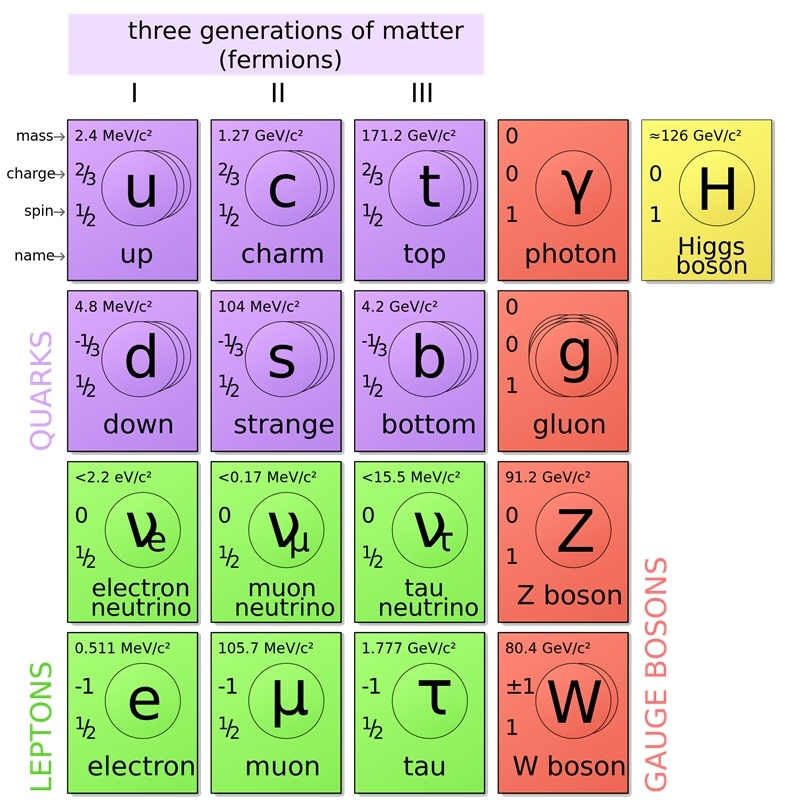
\includegraphics[scale=0.3]{Immagini/SM}
\caption{Particelle elementari del Modello Standard.}
\label{fig:SM}
\end{figure}

Il Modello Standard descrive la materia come composta da due tipi di particelle, entrambi fermioni con spin $\nicefrac{1}{2}$, {\em leptoni} e {\em quark}:

\begin{itemize}
\item i {\em leptoni} hanno carica elettrica intera e quelli conosciuti sono sei, suddivisi in tre generazioni di doppietti con massa crescente. Ogni doppietto è costituito da una particella con carica $Q=-1$ che ha interazioni elettrodeboli, rispettivamente l'elettrone $e$, il muone $\mu$ e il leptone tau $\tau$ nelle tre generazioni. Il doppietto \`e completato da una particella neutra chiamata {\em neutrino}, $\nu_e$, $\nu_{\mu}$ e $\nu_{\tau}$ rispettivamente, che interagisce solo per interazione debole.
\item Analogamente ai leptoni i {\em quark} sono organizzati in doppietti. In questo caso però la carica è frazionaria: la componente superiore del doppietto ha carica $Q=2/3$ ed \`e costituita dai quark $u$, $c$ e $t$ rispettivamente per le tre generazioni. La componente inferiore ha carica $Q=-1/3$ ed \`e costituita dai quark $d$, $s$ e $b$ rispettivamente per le tre generazioni. I quark interagiscono sia elettrodebole che forte e quest'ultima interazione è alla base della formazione di stati legati chiamati adroni, come ad esempio neutrone e protone.
\end{itemize}

Ad ognuna di queste particelle corrisponde una antiparticella che ha i numeri quantici opposti ma stessa massa e spin. Oltre alle antiparticelle il Modello Standard prevede l'esistenza dei {\em bosoni di gauge} e del {\em bosone di Higgs}. I primi sono i mediatori delle interazioni che, a loro volta, derivano dalle simmetrie insite nella teoria:

\begin{itemize}
\item il {\em fotone} \`e responsabile della mediazione dell'interazione elettromagnetica;
\item i {\em bosoni $W^{\pm}$} e $Z$, sono i mediatori dell'interazione debole; un'esempio in cui entra in gioco questa forza è il decadimento $\beta$. Questi bosoni, sono massivi, circa $80\GeVcc$ e $91\GeVcc$ rispettivamente.
\item I {\em gluoni} sono i mediatori dell'interazione forte.
\end{itemize}

Come detto precedentemente la forza gravitazionale non è descritta dal MS, ma risulta essere trascurabile nelle interazione tra particelle, in quanto la sua intensità, paragonata a quella delle altre tre forze, è vari ordini di grandezza inferiore. Nel MS le interazioni sono descritte come manifestazioni di simmetrie di gauge della Lagrangiana. Queste simmetrie non ammettono termini di massa per i bosoni di gauge poiché questo porterebbe alla rottura delle simmetrie stesse. Tuttavia \`e possibile introdurre un meccanismo di rottura spontanea della simmetria, detto {\em di Higgs}, da cui derivano i termini di massa per i bosoni di gauge e un ulteriore bosone scalare massivo, il {\em bosone di Higgs} H. Attraverso il meccanismo di Higgs vengono anche introdotti i termini di massa dei fermioni.

{\bf Aggiungere un paragrafetto sulle problematiche del MS (dark matter, teoria efficace a bassa energia etc.). Per questo si costruiscono gli acceleratori ...}

\section{Il Large Hadron Collider}
Il {\em Large Hadron Collider} o {\em LHC} è attualmente il più grande acceleratore di particelle mai costruito. Si trova presso il {\em CERN} ({\em European Organization for Nuclear Research}), collocato in un anello sotterraneo di 27~km nella regione di Ginevra (Svizzera). 

LHC \`e un collider adronico in grado di produrre interazioni protone-protone all'energia di $13\TeV$ nel centro di massa. \`E stato progettato con due anelli separati con campo magnetico opposto in modo che i fasci controrotanti possano essere costituiti da particelle con la stessa carica elettrica. Questa caratteristica, oltre ad altre, fa di LHC una macchina di frontiera di ineguagliata complessit\`a che ha richiesto una grande innovazione tecnologica. 

L'accelerazione dei protoni avviene a stadi come schematizzato in~Fig.~\ref{fig:LHC}: i protoni ottenuti da idrogeno gassoso sono inizialmente accelerati da un acceleratore lineare, LINAC2. Successvamente i protoni sono iniettati nel Proton Synchroton Booster (PSB) che aumenta l'energia fino a $1.4\GeV$ e, in seguito, grazie al Proton Synchrotron, raggiungono i $25\GeV$. In queste fasi i protoni vengono raggruppati in pacchetti distanti temporalmente $25\ns$ intervallo che che corrisponde alla frequenza di interazioni di $40\MHz$ a cui LHC opera. 
I protoni vengono infine accelerati fino ad energie di $450\GeV$ nel Super Proton Synchrotron (SPS) prima di essere iniettati nei due anelli di LHC in cui subiscono l'ultima fase di accelerazione fino all'energia di $13\TeV$ prima di farli collidere nei punti in cui sono collocati gli esperimenti.

Il {\em Compact Muon Solenoid} o {\em CMS} è uno dei principali esperimenti di LHC, assieme ad ALICE, ATLAS e LHCb. 

\begin{figure}
\centering
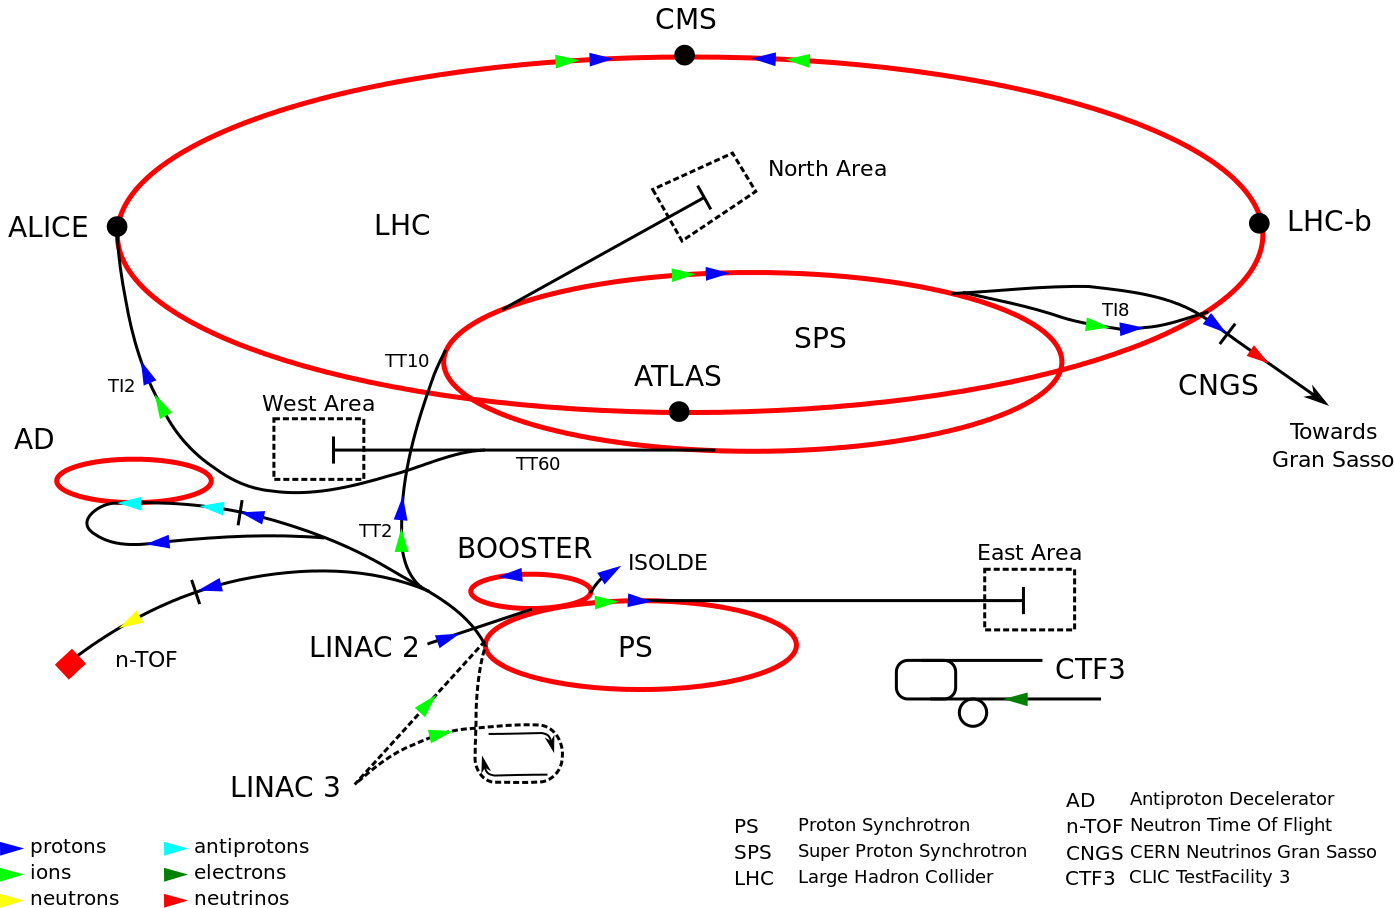
\includegraphics[scale=0.25]{Immagini/LHC}
\caption{Schema di pre-accelerazione e accelerazione di LHC.}
\label{fig:LHC}
\end{figure}

Lo scopo di questi esperimenti è lo studio del MS e la ricerca della materia oscura e di evidenze di nuova fisica, ovvero fenomeni non previsti dal MS stesso. Questi esperimenti sono collocati nei punti in cui i fasci di particelle si incrociano e le interazioni protone-protone prodotte possono essere quindi registrate ed essere analizzate in seguito. Pi\`u nel dettaglio:
\begin{itemize}
\item ALICE (A Large Ion Collider Experiment) \`e un esperimento che studia un stato della materia noto come {\em quark-gluon plasma}, prodotto nelle collisioni di ioni pesanti dal momento che, oltre alle collisioni protone-protone, LHC pu\`o operare come collisionatore ione-ione;
\item CMS (Compact Muon Solenoid) e ATLAS (A Toroidal LHC ApparatuS) sono entrambi progettati con lo scopo di investigare il più ampio spettro di fisica possibile. I due esperimenti hanno gli stessi obbiettivi, ma sono stati costruiti in modo differente al fine di essere indipendenti nello studio dei processi di interazione che avvengono durante le collisioni tra due protoni. Atlas e CMS nel 2012 hanno scoperto il bosone di Higgs~\cite{scopertahiggs}. 
\item LHCb (LHC beauty) \`e un esperimento che studia la fisica degli adroni contenenti il quark b e la violazione di CP (coniugazione di Carica e Parità) nelle interazioni elettrodeboli.
\end{itemize}
Altri esperimenti presenti ad LHC, ma di dimensioni minori sono TOTEM e LHCf:
\begin{itemize}
\item TOTEM (TOTal Elastic and diffractive cross section Measurement), ha come fine lo studio della fisica diffrettiva a piccolo angolo nelle interazioni protone-protone;
\item LHCf (LHC forward) è composto da due rivelatori che sono posizionati a $140$m dal punto di collisione di ATLAS per lo studio delle interazioni calorimetriche dei pioni neutri a grande rapidità\footnote{
Il sistema di coordinate convenzionalmente adottato dagli esperimenti LHC è tale che l'origine corrisponde al punto nominale di collisione dei due fasci con asse $y$ verticale orientato verso l'alto e asse $x$ in direzione radiale verso il centro di LHC. L'angolo azimutale $\phi$ è misurato a partire dall'asse $x$ e giace sul piano $x-y$ e la coordinata radiale su questo piano è $r$. L'angolo polare $\theta$ è misurato dall'asse $z$. 

Per lo studio dei processi è utile introdurre anche grandezze invarianti per trasformazioni di Lorentz come $\Delta {\rm y}$ e $\Delta \eta$, dove ${\rm y}$ indica la rapidità e $\eta$ la pseudorapidità:
\begin{equation}
{\rm y} = \dfrac{1}{2} ln\Big( \dfrac{E+p_z}{E-p_z}\Big)
\end{equation}

\begin{equation}
\eta = - ln \Big( tg\frac{\theta}{2}\Big)
\end{equation}
dove $E$ e $p_z$ sono rispettivamente l'energia e il momento lungo l'asse $z$ della particella prodotta. 
} e altissima energia, con lo scopo di verificare i modelli di simulazione per meglio modellizzare il comportamento dei raggi cosmici primari nell'interazione con l'atmosfera.
\end{itemize}

In un acceleratore due sono i parametri operativi fondamentali che ne determinano il potenziale di scoperta e la capacit\`a di effettuare accurate misure di fisica: l'energia del centro di massa e la luminosit\`a.

Pi\`u grande l'energia nel centro di massa, maggiore la massa delle particelle che possono essere prodotte e, in generale, a parit\`a di massa, \`e maggiore la sezione d'urto di produzione e quindi il numero di potenziali osservazioni. L'energia nel centro di massa di LHC \`e attualmente $\sqrt{s}=13\TeV$ a cui si \`e arrivati gradualmente: durante il RunI (2010-2012) l'energia del centro di massa \`e stata compresa tra 7 e $8\TeV$ ed \`e stata incrementata al valore attuale per il RunII (2015-2018). Durante il RunIII (2021-2023) l'energia del centro di massa raggiunger\`a $\sqrt{s}=14\TeV$.

La struttura non elementare dei protoni, costituiti internamente da partoni (quark e gluoni) che si dividono l'impulso totale, permette di produrre stati di energia intermedia fino al limite cinematico dell'energia del centro di massa e quindi di esplorare un ampio intervallo di energie senza dover modificare i parametri di funzionamento dell'acceleratore. Nella collisione l'interazione effettiva coinvolge solo una coppia di partoni che trasportano una frazione dell'impulso nominale dei due protoni. Questo costituisce un grande vantaggio dei collider adronici rispetto ai collider $\ee$ nell'ambito delle analisi di fisica di scoperta.

%che aumenta la probabilit\`a di produrre  motivo di una così alta energia è spiegato con la necessità di indagare processi fisici i cui effetti sono %maggiormente visibili se si è sopra una certa scala di energia. Un esempio è il Bosone di Higgs scoperto nel 2012, la cui massa è circa $125$ $GeV$.

Un ingrediente fondamentale per raggiungere energie elevate \`e il campo magnetico in cui sono immersi i tubi in cui circolano i fasci che sono inoltre tenuti ad una pressione di vuoto è di $10^{-13}{\mathrm atm}$, per evitare che i protoni interagiscano con le molecole di gas. Il campo magnetico, ortogonale al piano dell'anello, permette ai fasci di rimanere su una traiettoria quasi circolare. In particolare:
\begin{equation}
P[\GeVc] \sim 0.3 \cdot B[{\mathrm T}] \cdot r[\m]
\end{equation}
dove $B$ è il campo magnetico, $r$ il raggio di curvatura e $P$ l'impulso della particella. Dati i parametri di LHC ($r\sim4 \cdot 10^3\m$ e $P=6.5\TeVc$) si ottiene un campo $B$ che in media è pari a $\sim 5.4{\mathrm T}$. Per ottenere un campo di tale intensit\`a è stato necessario sviluppare dipoli magnetici superconduttori, il che ha rappresentato un'importante sfida tecnologica per la progettazione di LHC. Gran parte dell'anello di LHC, infatti, \`e mantentunto a temperature criogeniche di $\sim 2\degrees {\mathrm K}$ grazie ad un complesso sistema di raffreddamento.

Oltre all'energia nel centro di massa, la {\em luminosit\`{a} istantanea} ${\cal L}$ \`e il secondo importante parametro che
caratterizza le prestazioni di un collider. Infatti, il numero di eventi per unit\`a di tempo relativi ad un processo con sezione d'urto $\sigma$ \`e:
\begin{equation}
     \frac{dN}{dt} = \sigma {\cal L}.
\end{equation}
e, a parit\`a di sezione d'urto, maggiore la luminosit\`a istantanea, maggiore sar\`a la statistica potenzialmente disponibile per lo studio del processo. La luminosit\`a istantanea si misura in $\cm^{-2}\s^{-1}$ e, nel caso di collisioni centrali tra i pacchetti dei due
fasci, \`e data da:
\begin{equation}
   \label{for:luminos}
   {\cal L} = \frac{N_{1} N_{2} k f_{rev}}{4\pi \sigma _{x} \sigma _{y}}
\end{equation}
dove $N_{1}$ ed $N_{2}$ sono il numero di protoni nei due pacchetti collidenti (tipicamente $1--2\cdot10^{11}$), $k$ \`e il numero di pacchetti collidenti orbitanti nell'anello (per LHC normalmente compresi tra $\sim 2000$ e $\sim 2800$), $f_{rev}$ la loro frequenza di rivoluzione ($40\MHz$) e $\sigma_{x} \sigma_{y}$ \`e il prodotto delle standard--deviation delle gaussiane che rappresentano la distribuzione di densit\`a delle particelle dei pacchetti lungo le due dimensioni trasverse (per LHC $\sigma_{x}\sim\sigma_{y}\sim\um$).

Il numero di eventi $N$  di un dato processo prodotti in un certo intervallo di tempo $\Delta t$ \`e dato da 
\begin{equation}
     N = \sigma {\cal L}_{\rm int}
\end{equation}
dove ${\cal L}_{\rm int}$ \`e detta {\em luminosit\`{a} integrata} definita come la luminosit\`a raccolta nell'intervallo di tempo in oggetto:
\begin{equation}
   {\cal L}_{int} = \int_{\Delta t} {\cal L}\ dt.
\end{equation}

Dati i valori tipici ad LHC, la luminosit\`a integrata si misura in $\ifb$.

La luminosit\`a istantanea di LHC \`e salita gradualmente dall'inizio della presa dati nel 2010 come illustrato nella Fig.(
%{\em mettiamoci https://cms-service-lumi.web.cern.ch/cms-service-lumi/publicplots/peak_lumi_pp.png}
), dove \`e rappresentata la luminosit\`a istantanea di picco prodotta nel punto di interazione corrispondente all'esperimento CMS, fino a raggiungere il valore di $\sim 2\cdot10^{34}\cm^{-2}\s^{-1}$. L'andamento annuale della luminosit\`a integrata in funzione del tempo raccolta dall'esperimento CMS, al netto dell'efficienza dell'apparato, \`e mostrato in~Fig.(). Per le analisi di fisica, ad oggi, CMS ha a disposizione dati di collisione protone-protone pari a circa $130\ifb$ di luminosit\`a integrata. Alla fine del RunIII, che non vedr\`a aumenti significativi della luminosit\`a istantanea dato che i limiti operativi della macchina sono stati raggiunti, la luminosit\`a integrata totale raggiunta da CMS (come pure da Atlas) \`e stimabile in circa $300/ifb$.

Un parametro molto importante dal punto di vista sperimentale, e proporzionale alla luminosit`a istantanea, \`e il numero di collisioni pp simultanee (in gergo {\em pile up}) che hanno luogo durante un singolo bunch-crossing. Dato che dal punto di vista sperimentale si studia la singola interazione pp, l'esperimento deve essere idealmente in grado di isolare l'interazione di interesse da tutto il resto delle interazioni di pile-up. Ad oggi i valori di pile-up sperimentati da Atlas e CMS hanno raggiunto un valore medio di $\sim 40/\bx$ con picchi pari a $\sim 70/\bx$. Nonostante che gli esperimenti Atlas e CMS siano stati progettati per minimizzare gli effetti del pile-up, nella pratica i prodotti delle interazioni di pile-up, a causa delle risoluzioni sperimentali finite, possono essere confusi con i prodotti della interazione pp di interesse degradando quindi, per quest'ultima, la risoluzione delle osservabili fisiche.



\section{HL-LHC}
Il progetto {\em High Luminosity LHC} o {\em HL-LHC}, formalmente approvato nel Giugno 2016 dal CERN, prevede un aggiornamento della macchina LHC che porter\`a la luminosit\`a istantanea almeno fino ad un valore di riferimento pari a $\sim 5\cdot10^{34}\cm^{-2}\s^{-1}$ mentre l'energia del centro di massa rimarr\`a pari a $14\TeV$. Secondo scenari operativi pi\`u aggressivi, che sembrano comunque alla portata di HL-HLC, la luminosit\`a istantanea potrebbe raggiungere $\sim 7.5\cdot10^{34}\cm^{-2}\s^{-1}$. HL-LHC partir\`a nel 2026 e, nel corso di dieci anni di presa dati, ATLAS e CMS saranno quindi in grado di raccogliere luminosit\`a integrate comprese tra $\sim3000\ifb$ e $sim4500\ifb$. Dato che la spaziatura tra i pacchetti rimarr\`a di $25\ns$, il pile-up medio sar\`a compreso tra $140/\bx$ e $200/\bx$.

L'aumento della luminosit\`a istantanea seguir\`a a diverse migliorie dell'ottica di fascio ottenute rimpiazzando un centinaio di magneti corrispondenti a pi\`u di un km su $27\km$ di componenti di LHC. Di particolare importanza l'istallazione di nuovi quadrupoli posti in prossimit\`a dei punti di interazione di Atlas e CMS. Questi magneti superconduttori con tecnologia ${\rm Nb_3Sn}$, a differenza della pi\`u convenzionale NbTi, garantiranno una maggiore intensit\`a di campo (da 8 a $12\T$) e, grazie alla maggiore apertura, permetteranno un maggior fuocheggiamento dei fasci. 

I livelli di radiazione saranno senza precedenti: al centro di CMS, dove saranno istallati gli strati pi\`u interni del tracciatore a pixel, la fluenza equivalente a neutroni da un MeV sar\`a pari a $2.3\cdot 10^{16} {\rm neq}/\cm^2$ e la dose ionizzante totale (TID) a $12\MGy$ ($1.2\Grad$) al raggiungimento del valore di riferimento di luminosit\`a integrata pari a $3000\ifb$.

A seguito del potenziamento di LHC anche gli esperimenti dovranno essere aggiornati al fine di mantenere le prestazioni dei rivelatori in termini di efficienza, risoluzione, reiezione di processi di fondo ecc. nonostante l'aumento di radiazione e le più difficili condizioni operative.
In figura~\ref{HL-LHC} è mostrato un prospetto del programma di LHC fino a tutto il 2039 che contempla anche i prolungati intervalli di interruzione della presa dati ({\em Long Shutdown} o {\em LS}) necessari per la manutenzione e l'adeguamento di LHC e degli esperimenti. Il RunII, attualmente in corso, continuerà fino alla fine del 2018 quando inizierà il Long Shutdown 2 (LS2) a cui seguir\`a il RunIII. Durante il Long Shutdown 3 (LS3), dal 2024 fino alla metà del 2026, saranno eseguiti gli aggiornamenti principali di LHC e degli esperimenti per HL-LHC.
\begin{figure}
\centering
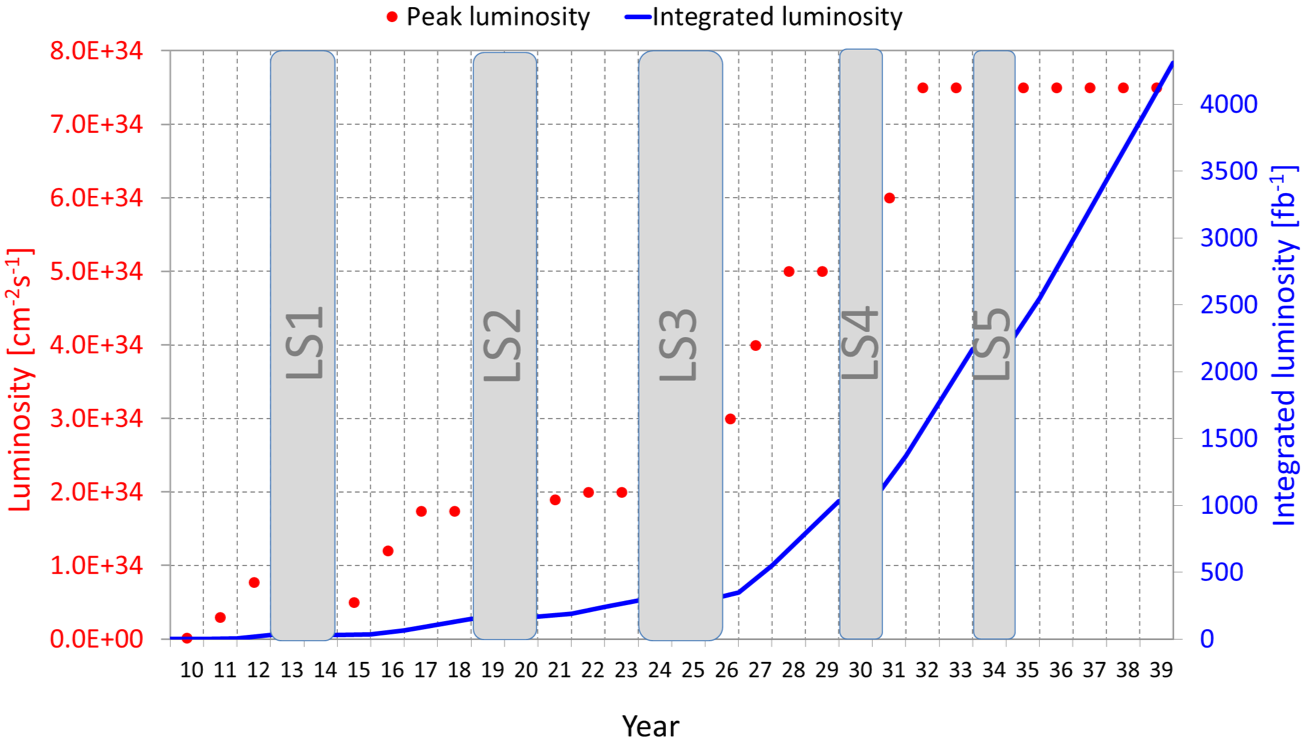
\includegraphics[scale=.35]{Immagini/LHC_lumi_2010_2039.png}
\caption{L'evoluzione della luminosit\`a istantanea e integrata di LHC fino al 2039 con i previsti periodi di interruzione della presa dati; LHCC P 008}
\label{HL-LHC}
\end{figure}

\subsection{Le motivazioni di fisica di HL-LHC}

HL-LHC amplier\`a enormemente il potenziale di fisica di LHC sia per le misure di precisione e per i processi rari nell'ambito del MS, sia per la portata di scoperta di processi previsti da teorie oltre il MS.
 
Un esempio \`e lo studio degli accoppiamenti di Yukawa del bosone di Higgs che, grazie a HL-LHC, potranno essere misurati da CMS con precisioni dell'ordine di qualche percento anche nel caso del muone che, con una frazione di decadimento di $\sim 10^{-4}$, \`e sperimentalmente ambizioso.
Il notevole miglioramento della precisione delle misure degli accoppiamenti del bosone di Higgs \`e illustrato in Fig.~\ref{HLLHCCouplings} nel confronto tra i risultati del RunI e la stima di quanto ottenibile a HL-LHC.
\begin{figure}
\centering
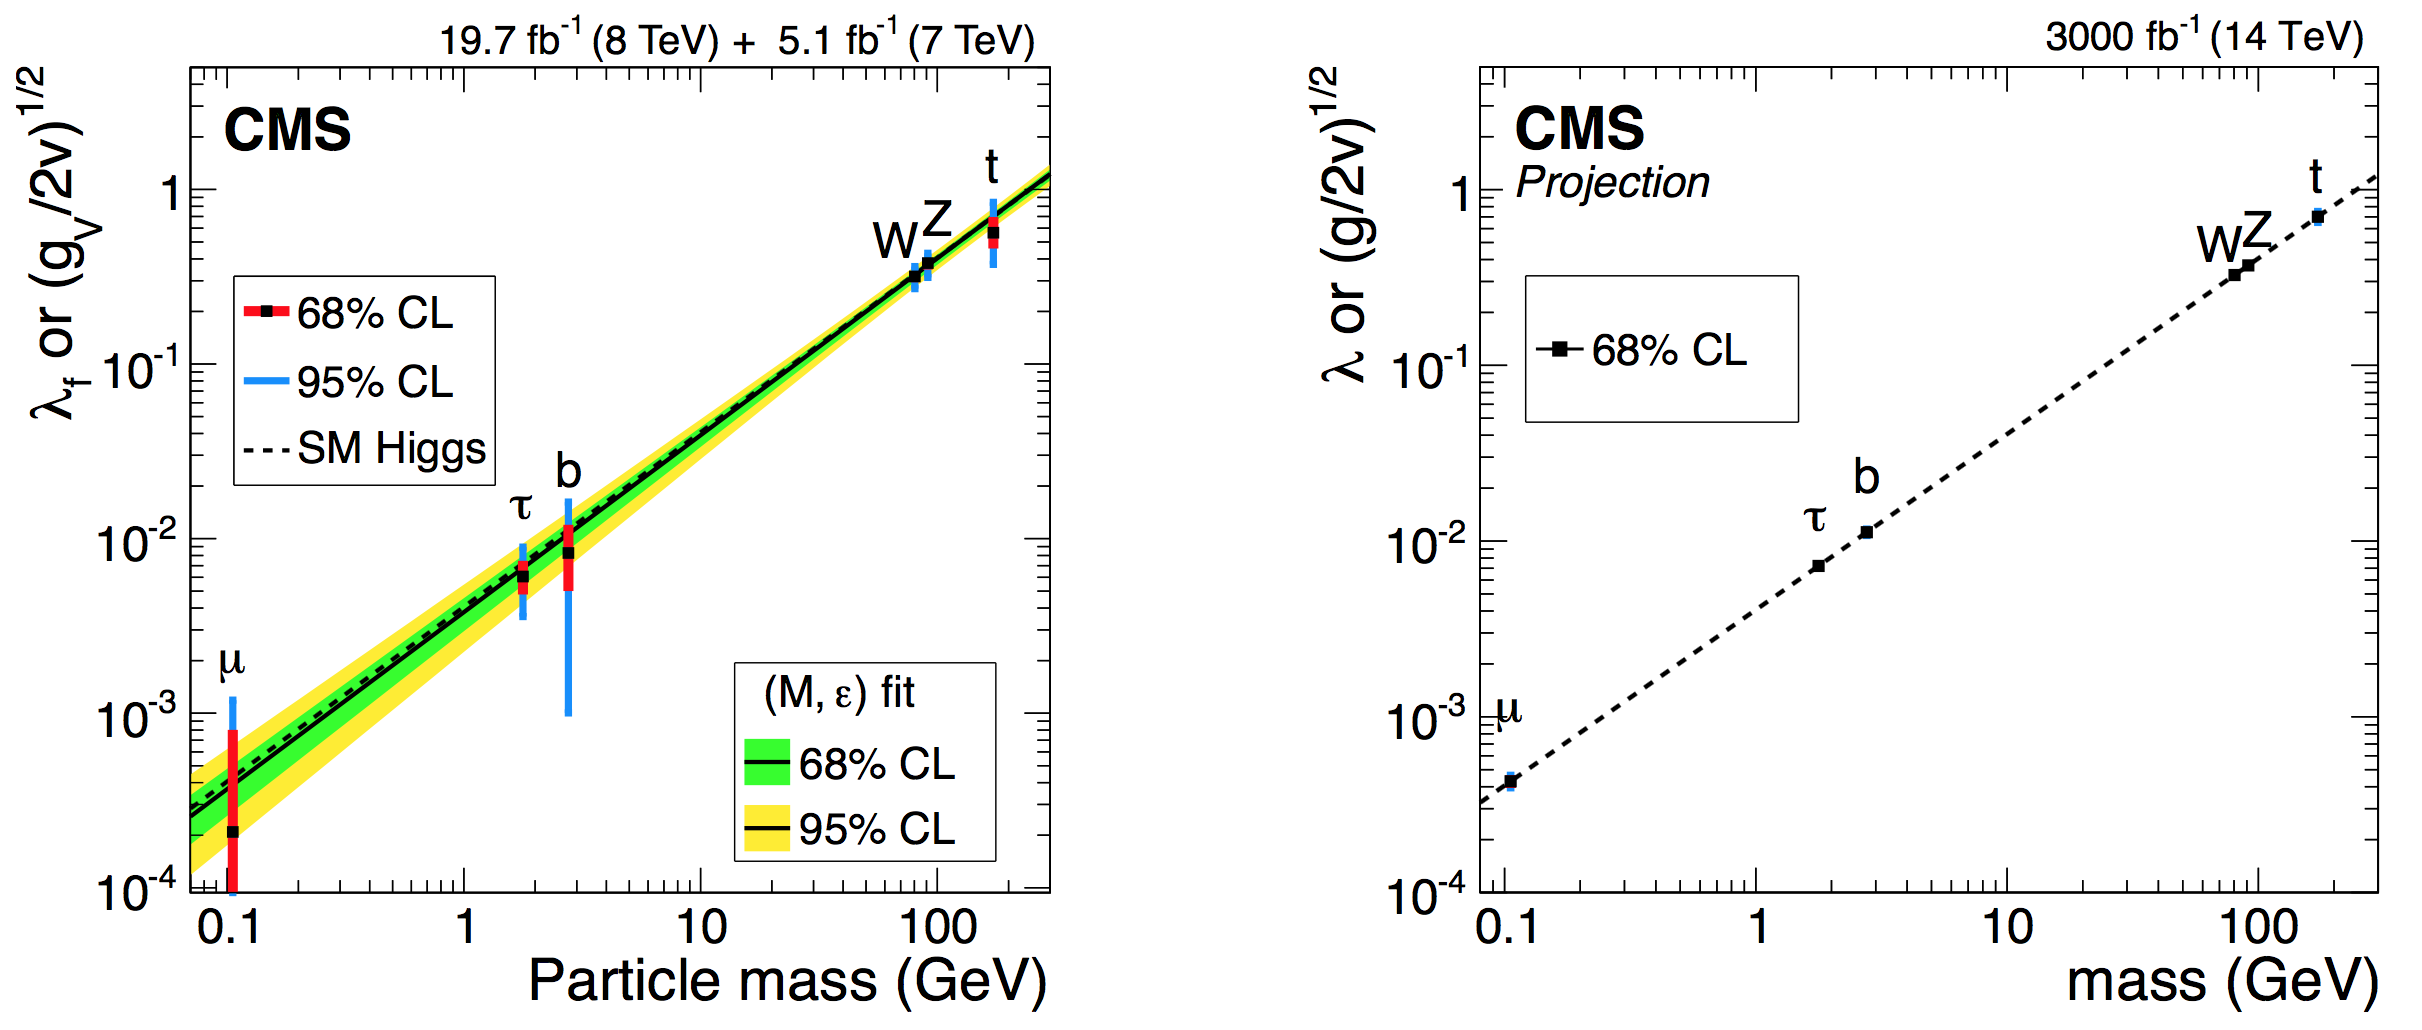
\includegraphics[scale=.35]{Immagini/HLLHC_Couplings.png}
\caption{Gli accoppiamenti del bosone di Higgs a fermioni e bosoni parametrizzati come $(g_V/2v)^{1/2}$, dove $v$ \`e il valore di aspettazione di vuoto de campo di Higgs in funzione della massa della particella; a sinistra le misure effettuate a RunI; a destra con l'estrapolazione delle incertezze a HL-LHC per $3000\ifb$ di luminosit\`a integrata assumendo gli accoppiamenti previsti dal MS.}
\label{HLLHCCouplings}
\end{figure}

Uno studio fondamentale \`e quello della produzione in coppie di Higgs, che permette di investigare i vertici trilineari con cui il bosone di Higgs interagisce con se stesso, come lo studio dei processi di scattering che coinvolgono i bosoni vettori deboli. Tutti questi processi sono intimamente legati alla rottura spontanea ella simmetria elettrodebole e al ruolo del bosone di Higgs stesso nel MS~\cite{vediTDRref13}. Eventuali deviazioni dalle previsioni del MS sarebbero indizio di nuova fisica oltre il MS stesso. Pur rappresentando una difficile sfida sperimentale per i fondi dominanti, se non irriducibili, e le piccole sezioni d'urto HL-LHC ne consentir\`a uno studio approfondito.

In questi ambiti \`e importante notare come la regione in avanti a grande pseudo-rapidit\`a sia sperimentalmente molto attraente perch\'e, dati i processi di produzione, vi si concentra una frazione non trascurabile del segnale. Si veda, a titolo di esempio, la Fig.~\ref{fig:VBFHtt_HH4b} relativa a processi tra i pi\`u interessanti dal punto di vista sperimentale: il processo H$\rightarrow \tau\tau$ in cui l'Higgs \`e prodotto per scattering di bosoni vettori ({\em Vector Boson Fusion}, VBF) e la produzione in coppia di bosoni di Higgs che decadono successivmante in coppie $\mathrm{b}\overline{\mathrm{b}}$, $\mathrm{HH}\rightarrow \mathrm{b}\overline{\mathrm{b}}\mathrm{b}\overline{\mathrm{b}}$. In entrambi i casi una accettanza di rivelazione estesa a grande pseudo-rapidit\`a permetterebbe di incrementare sensibilmente l'accettanza sperimentale per i processi in oggetto.
\begin{figure}[t]
\centering
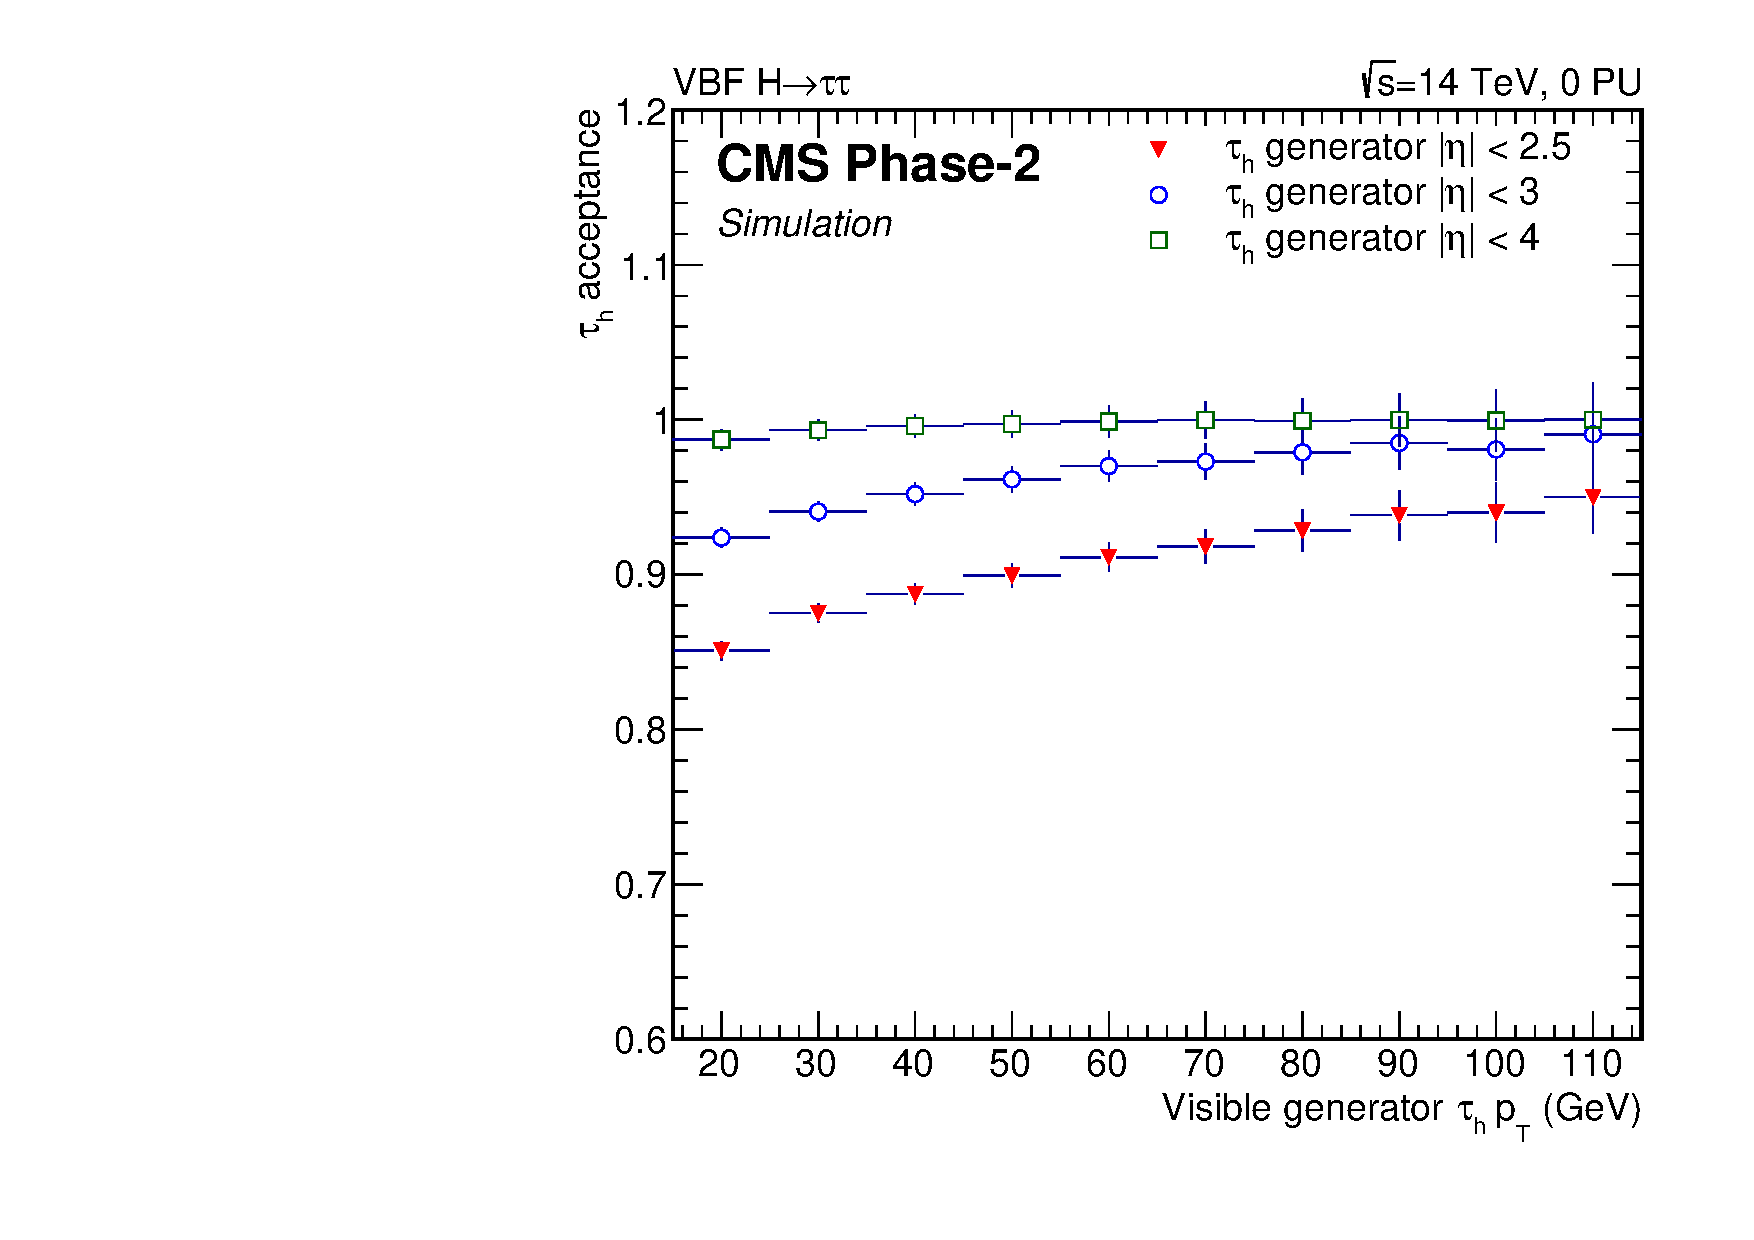
\includegraphics[width=0.45\textwidth]{Immagini/VBF_HTT_tau_acceptance.pdf}
\hfill
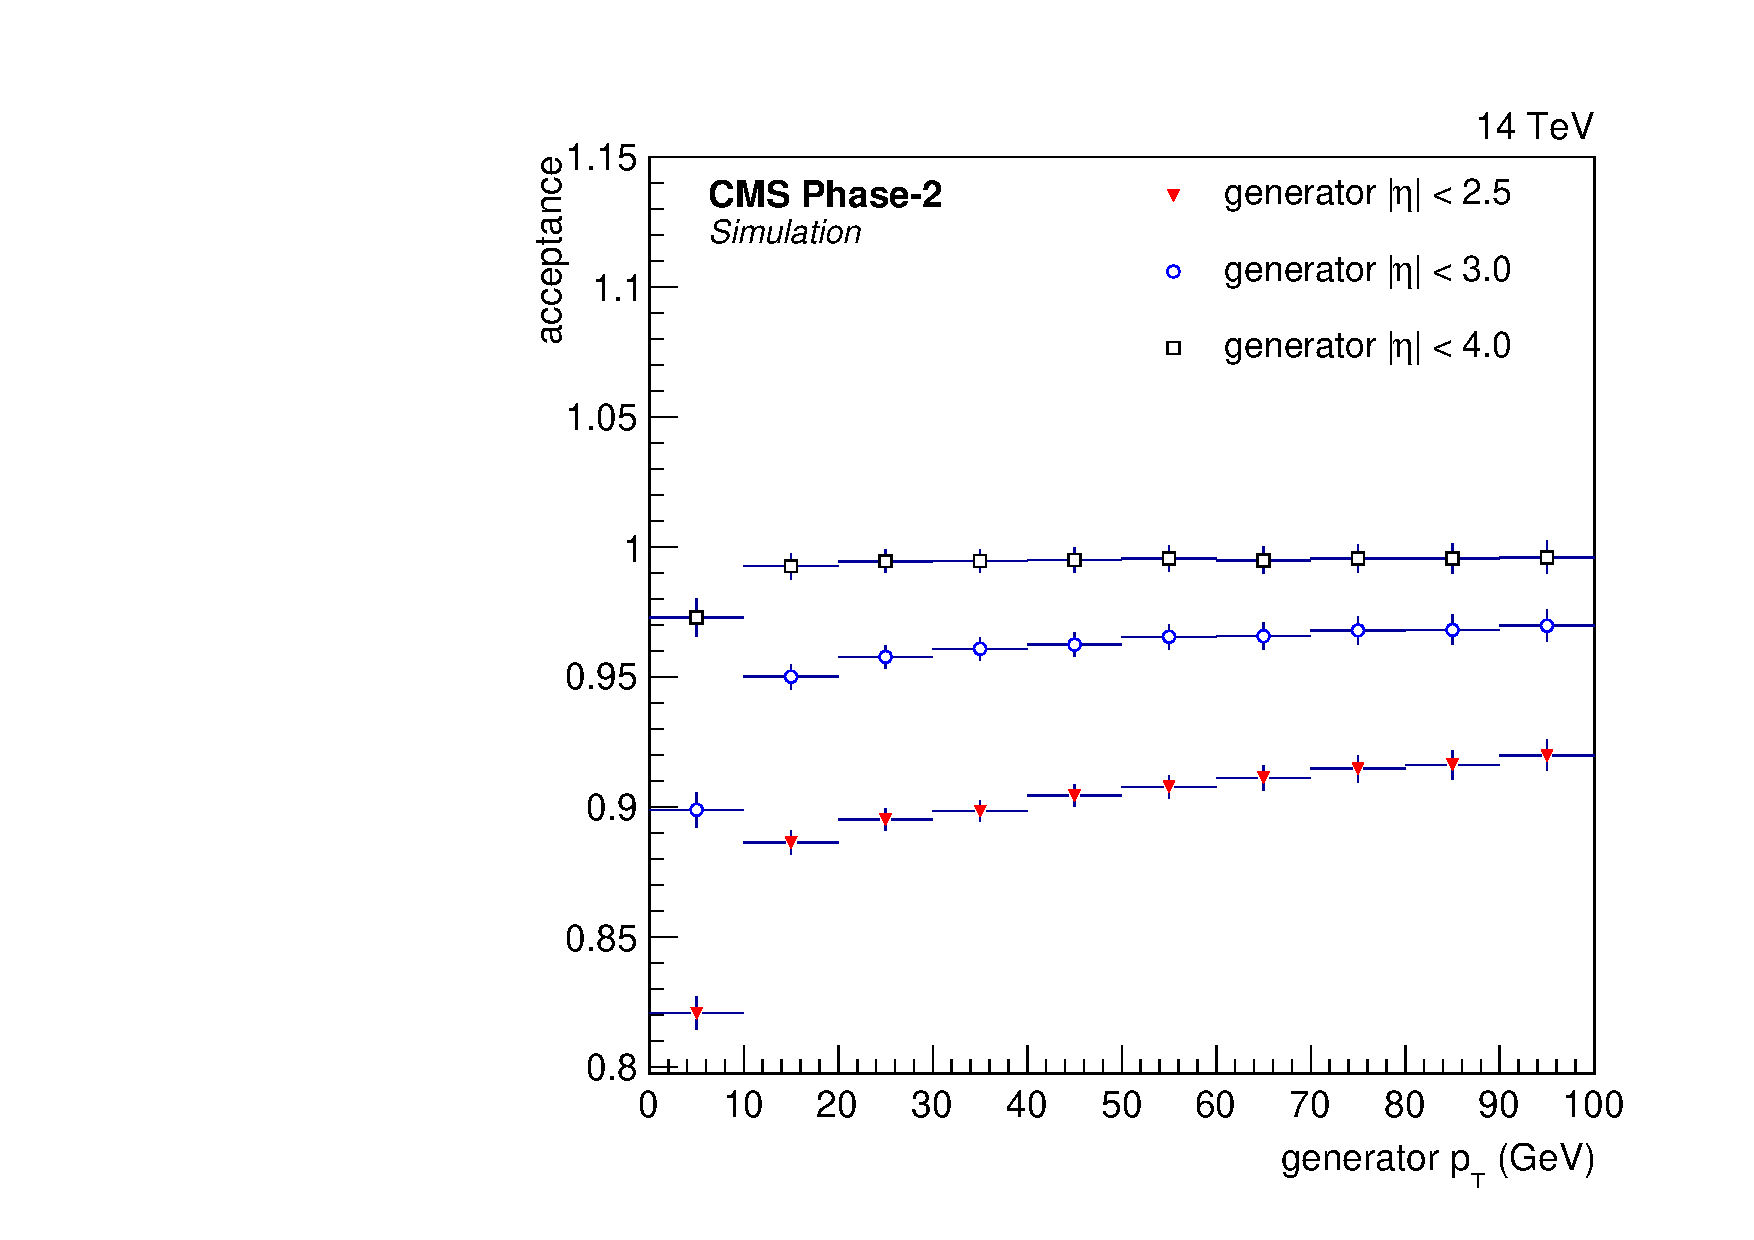
\includegraphics[width=0.45\linewidth]{Immagini/HH4b_acc.pdf}
\caption{Sinistra: accettanza relativa a leptoni $\tau$ che decadono adronicamente, $\tau_{\mathrm{h}}$, in funzione dell'impulso trasverso visibile  $\tau_{\mathrm{h}}$ $\pt$ generato nella simulazione per tre selezioni in pseudo-rapidit\`a; destra: frazione dei b-jet negli eventi di segnale, stimata con la simulazione, in funzione del $\pt$ del jet stesso per tre selezioni in pseudo-rapidit\`a. Per entrambe le figure le selezioni in pseudo-rapidit\`a sono $|\eta|<2.5$ (rosso), $|\eta|<3$ (blue) e $|\eta|<4$ (verde).
}
\label{fig:VBFHtt_HH4b}
\end{figure}

L'aumento di luminosit\`a, rendendo visibili processi con piccola sezione d'urto, amplier\`a il potenziale di scoperta di LHC per le ricerche dirette di nuove particelle previste dai modelli di estensione del MS ({\em beyond standard model} o BSM) inclusi quelli ritenuti pi\`u promettenti come la Supersimmetria e i modelli che prevedono extra-dimensioni o bosoni di gauge alla scala del TeV. Le ricerche indirette di nuova fisica che si basano sulla misura di decadimenti rari godranno di un analogo beneficio. Per esempio l'analisi del canale $B^0_s\to \mu \mu$ diventer\`a una misura di precisione e si stima che l'osservazione del decadimento $B_0\to\mu\mu$ sar\`a statisticamente solida con una significanza statistica di oltre 6 $\sigma$.

% \subsection{Obiettivi}

% L'idea di aumentare la luminosità di LHC oltre quella decisa nel progetto originale è antecedente alla messa in opera del progetto. Eventuali modifiche importanti alla macchina e agli esperimenti possono essere eseguite solo con lunghi periodi di shut down in cui è possibile accedere al tunnel e alle caverne. Per questo motivo è stato deciso un piano temporale che intervalli periodi di presa dati (Run I, Run II etc.) e periodi in cui si ha uno spegnimento completo per lunghi periodi (LS1, LS2, LS3). In figura \ref{HL-LHC} è possibile vedere la suddivisione temporale tra periodi di presa dati e periodi di spegnimento.
% Run I è stato il periodo di presa dati dal 2011 al 2012. Nel primo periodo di stop LS1 LHC è stato modificato al fine di raggiungere energie  nel centro di massa di 13 TeV, per poi arrivare gradualmente a 14 TeV. In questo momento siamo alla fine del Run II, e nell'esperimento CMS si  hanno una media di 25 interazioni per bunch, ciò vuol dire 25 vertici da ricostruire ogni 25 ns. Attraverso modifiche  e miglioramenti apportati nel LS1 e LS2 verrà aumentata la luminosità, questa parte del processo per l'esperimento CMS va sotto il nome di fase-I. Durante il periodo LS3  saranno invece sostituite vari parti degli esperimenti, che a causa del danneggiamento da radiazione saranno deteriorati e nello contemporaneamente verranno sostituiti i quadrupoli di fuocheggiamento con nuovi modelli capaci di incrementare la luminosità. 
% Il periodo che seguirà LS3 sarà chiamato fase II o HL-LHC (High Luminosity LHC). Nello scenario prefissato la lumiosità istantanea sarà di $5 \cdot 10 34 cm^{-2} s^{-1}$ con picchi di $2 \cdot 10 35 cm^{-2} s^{-1}$, in questo modo gli esperimenti saranno in grado di raccogliere una maggiore statistica con una luminosità di $300 fb^{-1}$ ogni anno per 10 anni(250 o 300)?????%at 5 × 10 34 cm − 2 s − 1 from a potential peak value of 2 × 10 35 cm − 2 s − 1 at the beginning of fills,
% %and to deliver 250 fb − 1 per year for a further 10 years of operation. Under these conditions
% In queste condizioni ci sarà una maggiore probabilità di sovrapposizione di interazioni (Pile Up), questa sarà la grande sfida, insieme alla gestione degli effetti di degradazione in cui incorreranno i rivelatori a seguito delle maggiori dosi di radiazione assorbita. Sempre nella figura \ref{HL-LHC} è possibile vedere le proiezioni di luminosità di picco e luminosità integrata.
 
% %The high luminosity period that follows LS3 with the upgraded LHC is referred to here as HL-LHC or Phase-II. The proposed operating scenario is to level the instantaneous luminosity
% %at 5 × 10 34 cm − 2 s − 1 from a potential peak value of 2 × 10 35 cm − 2 s − 1 at the beginning of fills,
% %and to deliver 250 fb − 1 per year for a further 10 years of operation. Under these conditions the event PU will rise substantially to become a major challenge for the experiments, and the performance degradation due to integrated radiation dose will need to be addressed. This Technical Proposal presents the CMS upgrade program for Phase-II. The schedule of beam operations and long shutdowns, together with projections of the peak and integrated luminosities, is shown in Fig. 1.9, and is, of course, subject to change.

\chapter{L'esperimento CMS}

\section{I sottosistemi di CMS}

Il {\em Compact Muon Solenoid} (CMS) [CMS Collaboration The CMS experiment at LHC JINST 08 (2008) 03] \`e un esperimento polivalente per lo studio generale delle collisioni pp fino ad un’energia di $14\TeV$. Il rivelatore \`e infatti ottimizzato per misurare energia e impulso delle particelle prodotte durante le collisioni. Per garantire la massima ermeticit\`a, l’apparato sperimentale ha una struttura centrale approssimativamente cilindrica, detta {\em barrel}, sigillata ad entrambe le estremit\`a da strutture di chiusura dette {\em endcap} per un diametro complessivo di $15\m$, una lunghezza di $\sim22\m$ e $\sim 12500$ tonnellate di peso. La capacit\`a di identificazione delle particelle prodotte \`e assicurata dai diversi tipi di sotto-rivelatori disposti in strati rispetto al punto di incrocio dei fasci come schematicamente mostrato in Fig.~\ref{fig:spaccatoCMS}: pi\`u internamente i tracciatori di particelle cariche ovvero il rivelatore a pixel di silicio e il rivelatore a microstrip di silicio; all'esterno di quest'ultimo abbiamo il calorimetro elettromagnetico e il calorimetro adronico; il tracciatore e i calorimetri sono collocati all’interno del magnete solenoidale superconduttore che genera un campo magnetico di $3.8\T$ parallelo all'asse dei fasci. Pi\`u esternamente, immerse nel ferro del giogo di ritorno del magnete, si trovano le camere a muoni.
\begin{figure}
\centering
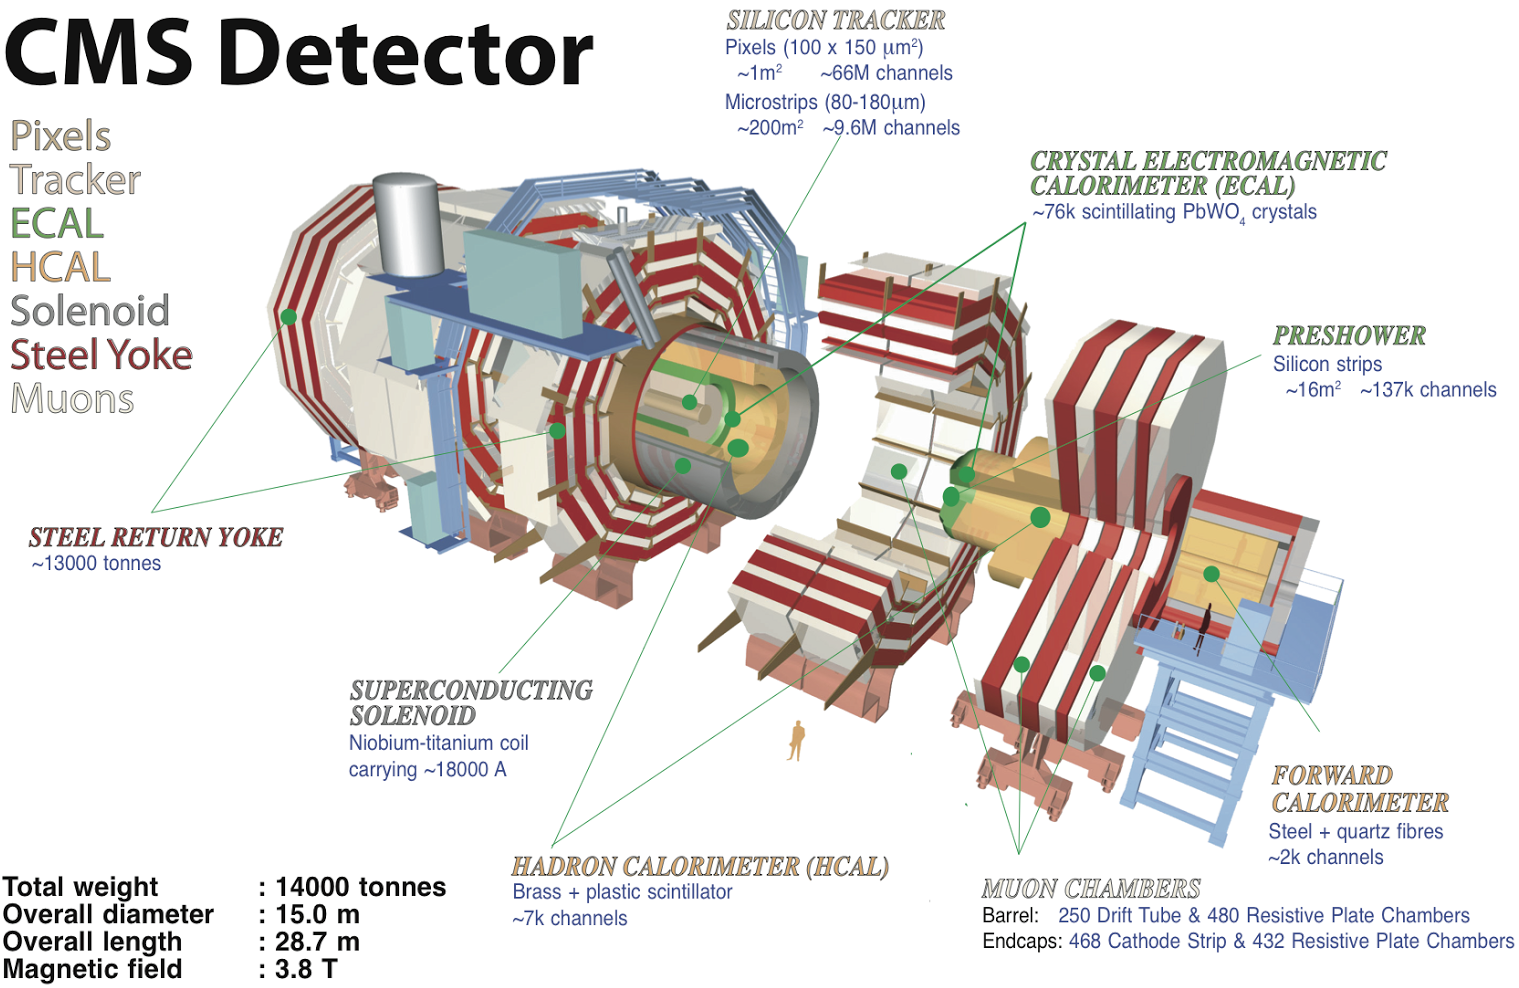
\includegraphics[width=\textwidth]{Immagini/cms_3d.png}
\caption{Vista dello spaccato dell'attuale esperimento CMS in cui sono schematicamente visibili i vari sotto-rivelatori.}
\label{fig:spaccatoCMS}
\end{figure}

L’esperimento \`e collocato in una caverna alla profondit\`a di $\sim 100 m$ in corrispondenza del punto di interazione numero 5 di LHC (IP5). 

Pi\`u nel dettaglio gli attuali sotto-sistemi dell'esperimento CMS sono i seguenti, procedendo dal punto di interazione verso l'esterno:

\begin{description}
\item[Il tracciatore al silicio.] L'apparato in grado di ricostruire la traiettoria delle particelle cariche fino a $|\eta|<2.5$ misurandone l'impulso trasverso (grazie alla presenza del campo magnetico dato che $\pt [\GeV] = 0.3 B [\T] \rho [\m]$, dove $\rho$ \`e il raggio di curvatura) e individuando i vertici primari di interazione pp e gli eventuali vertici secondari di decadimento di particelle instabili prodotte dall'interazione; occupa il volume $r<1.2\m$, $|z|<250\cm$. \`E composto da due sottorivelatori: un rivelatore di vertice a pixel di silicio e un rivelatore a microstrip di silicio. Si veda la sezione~\ref{} per maggiori dettagli.
\item[ECAL.] Il calorimetro elettromagnetico (ECAL) misura l’energia di elettroni e fotoni fino a $|\eta|<3$. Collocato esternamente al tracciatore, \`e un calorimetro omogeneo composto da $\sim 76000$ cristalli scintillanti di tungstato di piombo (PbWO$_4$) di lunghezza equivalente a $\sim 25--26X_0$.
\item[HCAL.] Il calorimetro adronico (HCAL) misura l'energia delle particelle che interagiscono adronicamente fino a $|\eta|<5$ ed \`e. \`E un calorimetro ermetico a campionamento situato a valle di ECAL, rispetto al punto di interazione, composto da strati di ottone e di scintillatore plastico, corrispondenti a $7-11$ lunghezze d'interazione, e integrato da uno strato di scintillatore posto all'esterno del magnete nella parte barrel che ne aumenta lo spessore efficace per il contenimento degli sciami adronici.
\item[Il magnete superconduttore.] Il campo magnetico che deflette le particelle cariche cos\`i da stimarne l’impulso dalla curvatura \`e generato da un magnete superconduttore solenoidale lungo $13\m$, con un diametro interno di $6\m$, costituito da un un avvolgimento di cavo di NbTi in matrice di alluminio mantenuto alla temperatura di $4\degrees\K$ da un sistema criogenico. Il campo magnetico ha una intensit\`a nominale di $3.8\T$ corrispondenti a $\sim 20\kA$ di corrente,  di intensit\`a richiede circa $20\kA$ di corrente. Le linee di campo sono richiuse tramite un giogo esterno di $10000$ tonnellate di ferro.
\item[Le camere a muoni.] Il giogo di ritorno del magnete \`e attrezzato con rivelatori dedicati alla tracciatura dei muoni grazie anche al campo residuo di $1.8\T$ presente nel giogo. Nella parte barrel ci sono camere a deriva ({\em drift chamber}) e CSC ({\em cathode strip chamber}) negli endcap, in entrambi i casi integrati con RPC ($resistive plate chamber$).  
\end{description}

Una rappresentazione schematica dei differenti meccanismi di interazione delle varie particelle nei sotto-rivelatori, sui quali l'identificazione delle stesse \`e basata, \`e visibile in Fig.~\ref{fig:spicchioCMS}.
\begin{figure}
\centering
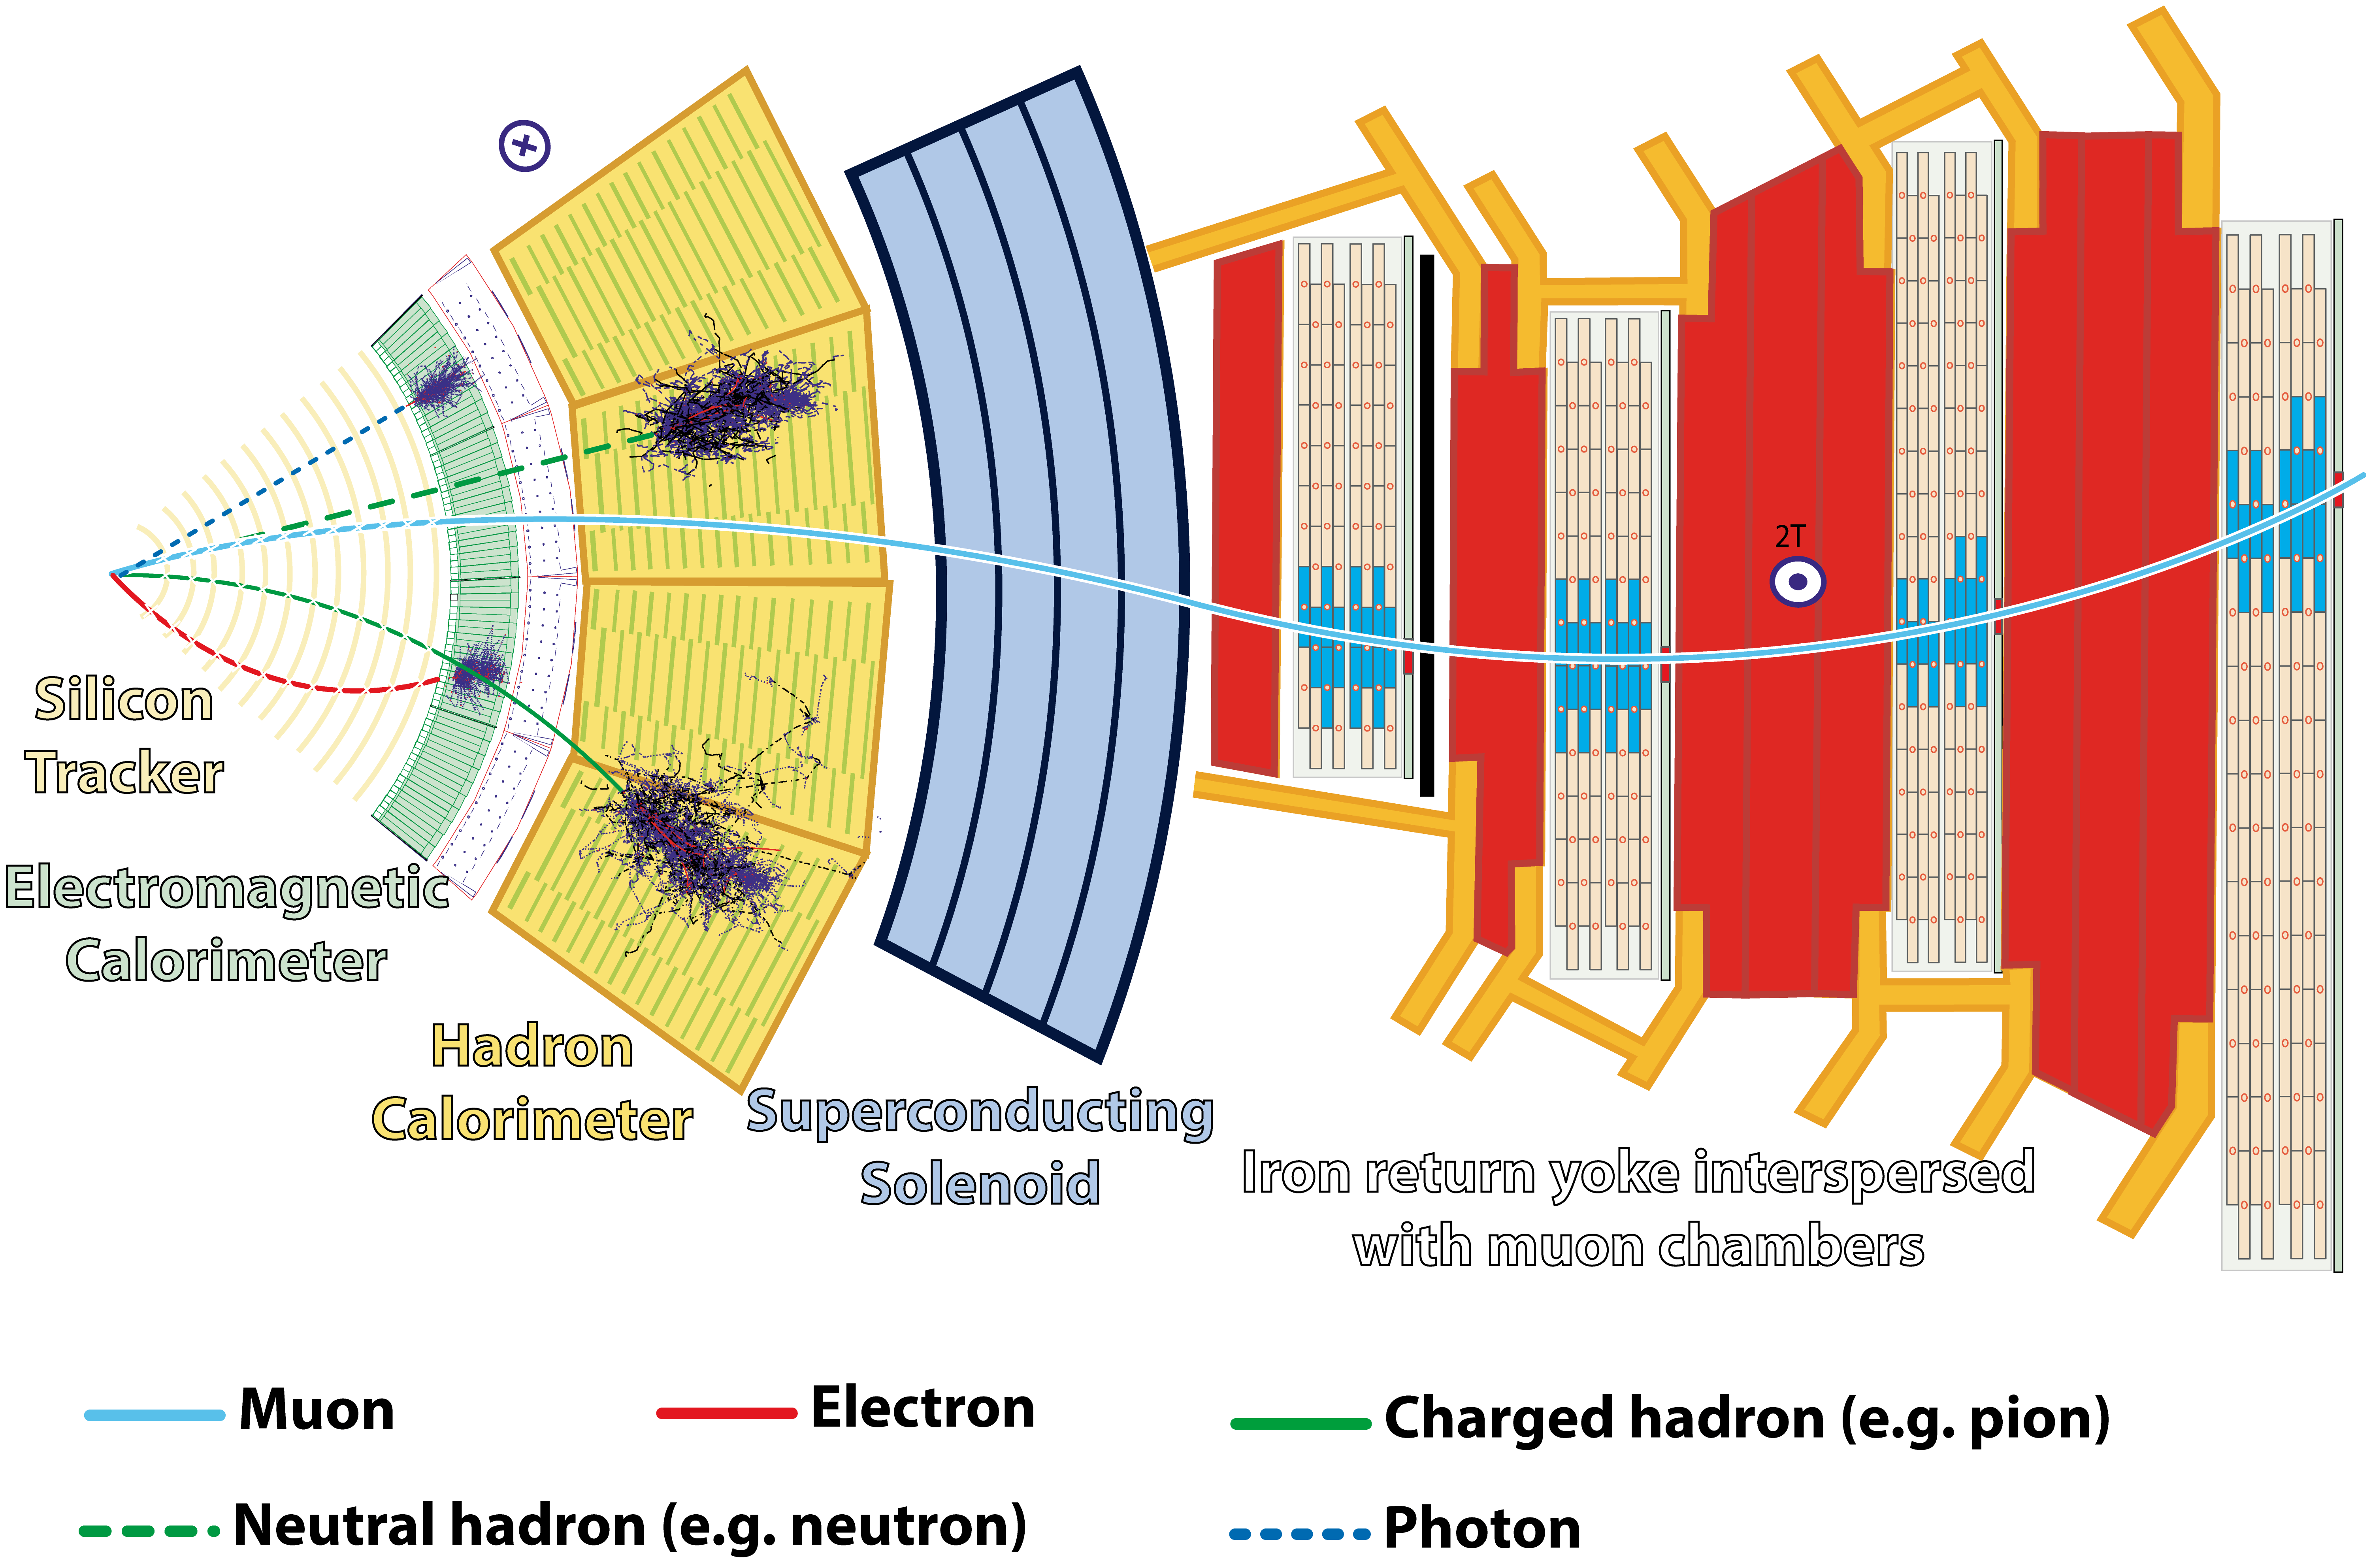
\includegraphics[scale=0.8]{Immagini/CMSbis}
\caption{Spaccato di CMS e risposta ai vari tipi di particella.}
\label{CMSbis}
\end{figure}

La frequenza di $40\MHz$ con cui avvengono i bunch crossing a LHC rende impraticabile il trasferimento integrale per ogni evento dei dati relativi ai $>100$M di canali di lettura di tutto CMS ({\em readout}). Sarebbe inoltre impossibile l'immagazzinamento di questa informazione data l'entit\`a delle memorie di massa che sarebbero richieste. Gli eventi di collisione sono quindi preventivamente filtrati da un sistema di {\em trigger} organizzato in due livelli di crescente complessit\`a che permettono di selezionare gli eventi interessanti per la fisica rispettando le limitazioni del readout e dell'archiviazione a lungo termine dei dati raccolti.

Il primo livello, detto {\em trigger di livello 1} (L1), sfrutta una lettura speciale a bassa risoluzione e granularit\`a dei rivelatori intrinsecamente veloci, ovvero calorimetri e camere a muoni. Questa informazione viene elaborata entro pochi microsecondi ({\em latenza}) compatibilmente con la profondit\`a temporale delle memorie tampone ({\em pipeline}) dell'elettronica di lettura di prossimit\`a ({\em front-end}) di tutti i sotto-rivelatori, che immagazzinano i dati in attesa dell'esito della selezione di L1. Questa \`e basata su semplici tagli sulle osservabili fisiche ricavabili dai dati disponibili al sistema di trigger di L1. La frequenza media di consenso del L1 \`e dell'ordine di qualche decina di $\kHz$.

Con il consenso di L1 tutta l'informazione di CMS relativa all'evento selezionato viene letta, digitalizzata e compressa. L'evento, che a questo punto ha una dimensione di $\sim2$MB, viene indirizzato all'{\em High Level Trigger}, HLT. L'HLT \`e una batteria di normali PC commerciali che, grazie alla pesante parallelizzazione e all'utilizzo di flessibili algoritmi semplificati, sono in grado di analizzare e filtrare ulteriormente gli eventi in tempo reale selezionando, con una frequenza media di qualche centinaio di Hz, quelli meritevoli di essere registrati indefinitamente per l'analisi.

Per HL-LHC CMS subir\`a un ampio potenziamento. Oltre alla sostituzione integrale del tracciatore, discussa in dettaglio pi\`u avanti, anche la calorimetria in avanti verr\`a migliorata con l'istallazione di un calorimetro a campionamento basato su sensori di silicio e scintillatore in una matrice di acciaio. Tutti gli altri sotto-sistemi vedranno modifiche nell'elettronica di lettura per soddisfare alle condizioni operative di HL-LHC. Il sistema di trigger verr\`a anch'esso migliorato: la frequenza di L1 aumenter\`a a $750\kHz$ con una latenza di $\sim 12.5\us$ per permettere l'elaborazione di un'informazione maggiore. Si prevede che, a valle dell'HLT, si scriveranno su disco circa $7.5k$ eventi al secondo.

%-------------------------

% Questa struttura rispecchia la necessità di ricostruire con precisione gli eventi originati dalla collisione di particelle, che avvengono in rapida successione. CMS come anche gli altri esperimenti, può essere paragonato ad una gigantesca macchina fotografica che registra 40 milioni di foto al secondo (digitalizzando l'informazione di decine di milioni di sensori). 
% La struttura a strati consente di avere rivelatori diversi in ogni strato, di cui i più interni sono meno densi, mentre i più esterni sono più densi. Questo perché il tracciatore non deve alterare l'energia delle particelle che poi sarà misurata nei calorimetri e per facilitare la ricostruzione delle tracce è importante evitare fenomeni di multiple scattering.

% Le particelle che gli scienziati cercano di riprodurre nelle collisioni protone-protone hanno vite medie molto brevi, e decadono rapidamente in particelle più leggere. Dopo un processo di hard-scattering migliaia di queste particelle leggere sono generate elettroni, muoni, fotoni, ma anche protoni, neutroni etc. Tutte queste particelle attraversano i vari strati di cui è composto il rivelatore. 
% Le informazioni raccolte vengono utilizzate per ricostruire l'evento di interazione, per  dedurre l'esistenza di nuove particelle.


% Le traiettorie delle particelle cariche sono piegate dal campo magnetico, e il loro raggio di curvatura è utilizzata per calcolare il loro impulso: maggiore è la loro energia cinetica, minore è la curvatura. Un'altra componente importante di un rivelatore sono i calorimetri per misurare l'energia delle particelle (sia cariche che non). 
% I calorimetri devono essere abbastanza grandi per assorbire anche le particelle più energetiche. Questi motivi fanno sì che gli esperimenti ad LHC siano così grandi. I rivelatori sono costruiti in modo il più possibile ermetico per raccogliere tutti i prodotti delle interazioni e poter ricostruire gli eventi. 
% Combinando le informazioni di ogni strato del rivelatore è possibile determinare il tipo di particella che ha lasciato una data traccia.

% Particelle cariche come elettroni, protoni e muoni, lasciano tracce ionizzando il materiale attraversato. Gli elettroni sono molto leggeri e perciò perdono energia velocemente, mentre i protoni penetrano più in profondità negli strati del rivelatore. I fotoni essendo neutri non rilasciano segnali nel tracciatore, ma nei calorimetri sono convertiti in elettroni e positroni e così ne viene misurata l'energia. 
% L'energia dei neutroni viene invece misurata indirettamente, trasferiscono l'energia ai protoni, che poi sono misurati. I muoni insieme ai neutrini (che non vengono rivelati) sono i soli a raggiungere gli strati più esterni.


% Ogni parte del rivelatore è connessa ad un sistema di lettura elettronico attraverso migliaia di cavi. Ogni volta che un segnale è raccolto, il sistema registra la sua posizione e l'istante in cui è stato raccolto, se il sistema di trigger decide che l'evento che ha generato Se tale segnale è di interesse, allora l'informazione è letta e portata all'esterno del rivelatore per essere utilizzata nelle analisi offline.
% Ci sono differenti criteri per selezionare un evento potenzialmente di interesse, in questo modo la mole enorme di eventi registrati in un secondo viene ridotta a poche centinaia, che poi verranno analizzate in dettaglio.


\section{L'attuale Tracciatore al Silicio di CMS}

Il tracciatore al silicio di CMS attualmente istallato merita una descrizione pi\`u approfondita per introdurre le motivazioni e i miglioramenti del potenziamento previsto per HL-LHC oggetto di questo lavoro di tesi.

Il tracciatore al silicio \`e il rivelatore di CMS pi\`u interno: \`e lungo $\sim6\m$ e ha un diametro esterno di $\sim 2.6\m$ ed \`e composto da un barrel centrale e da due endcap finali in modo tale da avere la massima ermeticit\`e fino a $|\eta|<2.5$.

La particella carica rilascia energia nel sensore di silicio che non \`e altro che un diodo contropolarizzato, per avere un volume di raccolta essenzialmente privo di portatori di carica. La carica di ionizzazione che segue al rilascio di energia viene raccolta dagli elettrodi di giunzione. Un elettrodo di giunzione finemente segmentato permette di avere informazione sulla posizione di passaggio della particella carica.

Il disegno del tracciatore \`e caratterizzato da: un’alta granularit\`a, soprattutto vicino al punto di interazione, dove il flusso di particelle \`e maggiore, per avere risoluzione in impulso e un'ottima ricostruzione di tracce limitando, in media, la frazione di canali interessati dal segnale ({\em occupancy}); un elevato e ridondante numero di punti misurati per traccia, per mitigare le conseguenze di possibili malfunzionamenti.

La temperatura di lavoro del tracciatore di CMS \`e compresa tra $-10\degrees$C e $-20\degrees$C per tenere sotto controllo gli effetti del danneggiamento da radiazione.
  
% una quantit`a non eccessiva di materiale da attraversare, che deteriora la precisione delle misure a causa dei fenomeni di scattering multiplo e della perdita di energia nel materiale.
Il tracciatore di CMS, schematicamente rappresentato in Fig.~\ref{fig:CMSTk}, \`e infatti composto di due sotto-rivelatori: il rivelatore a pixel con sensori pi\`u segmentati all'interno e il rivelatore a microstrip pi\`u esternamente. 
  
\begin{figure}
\centering
%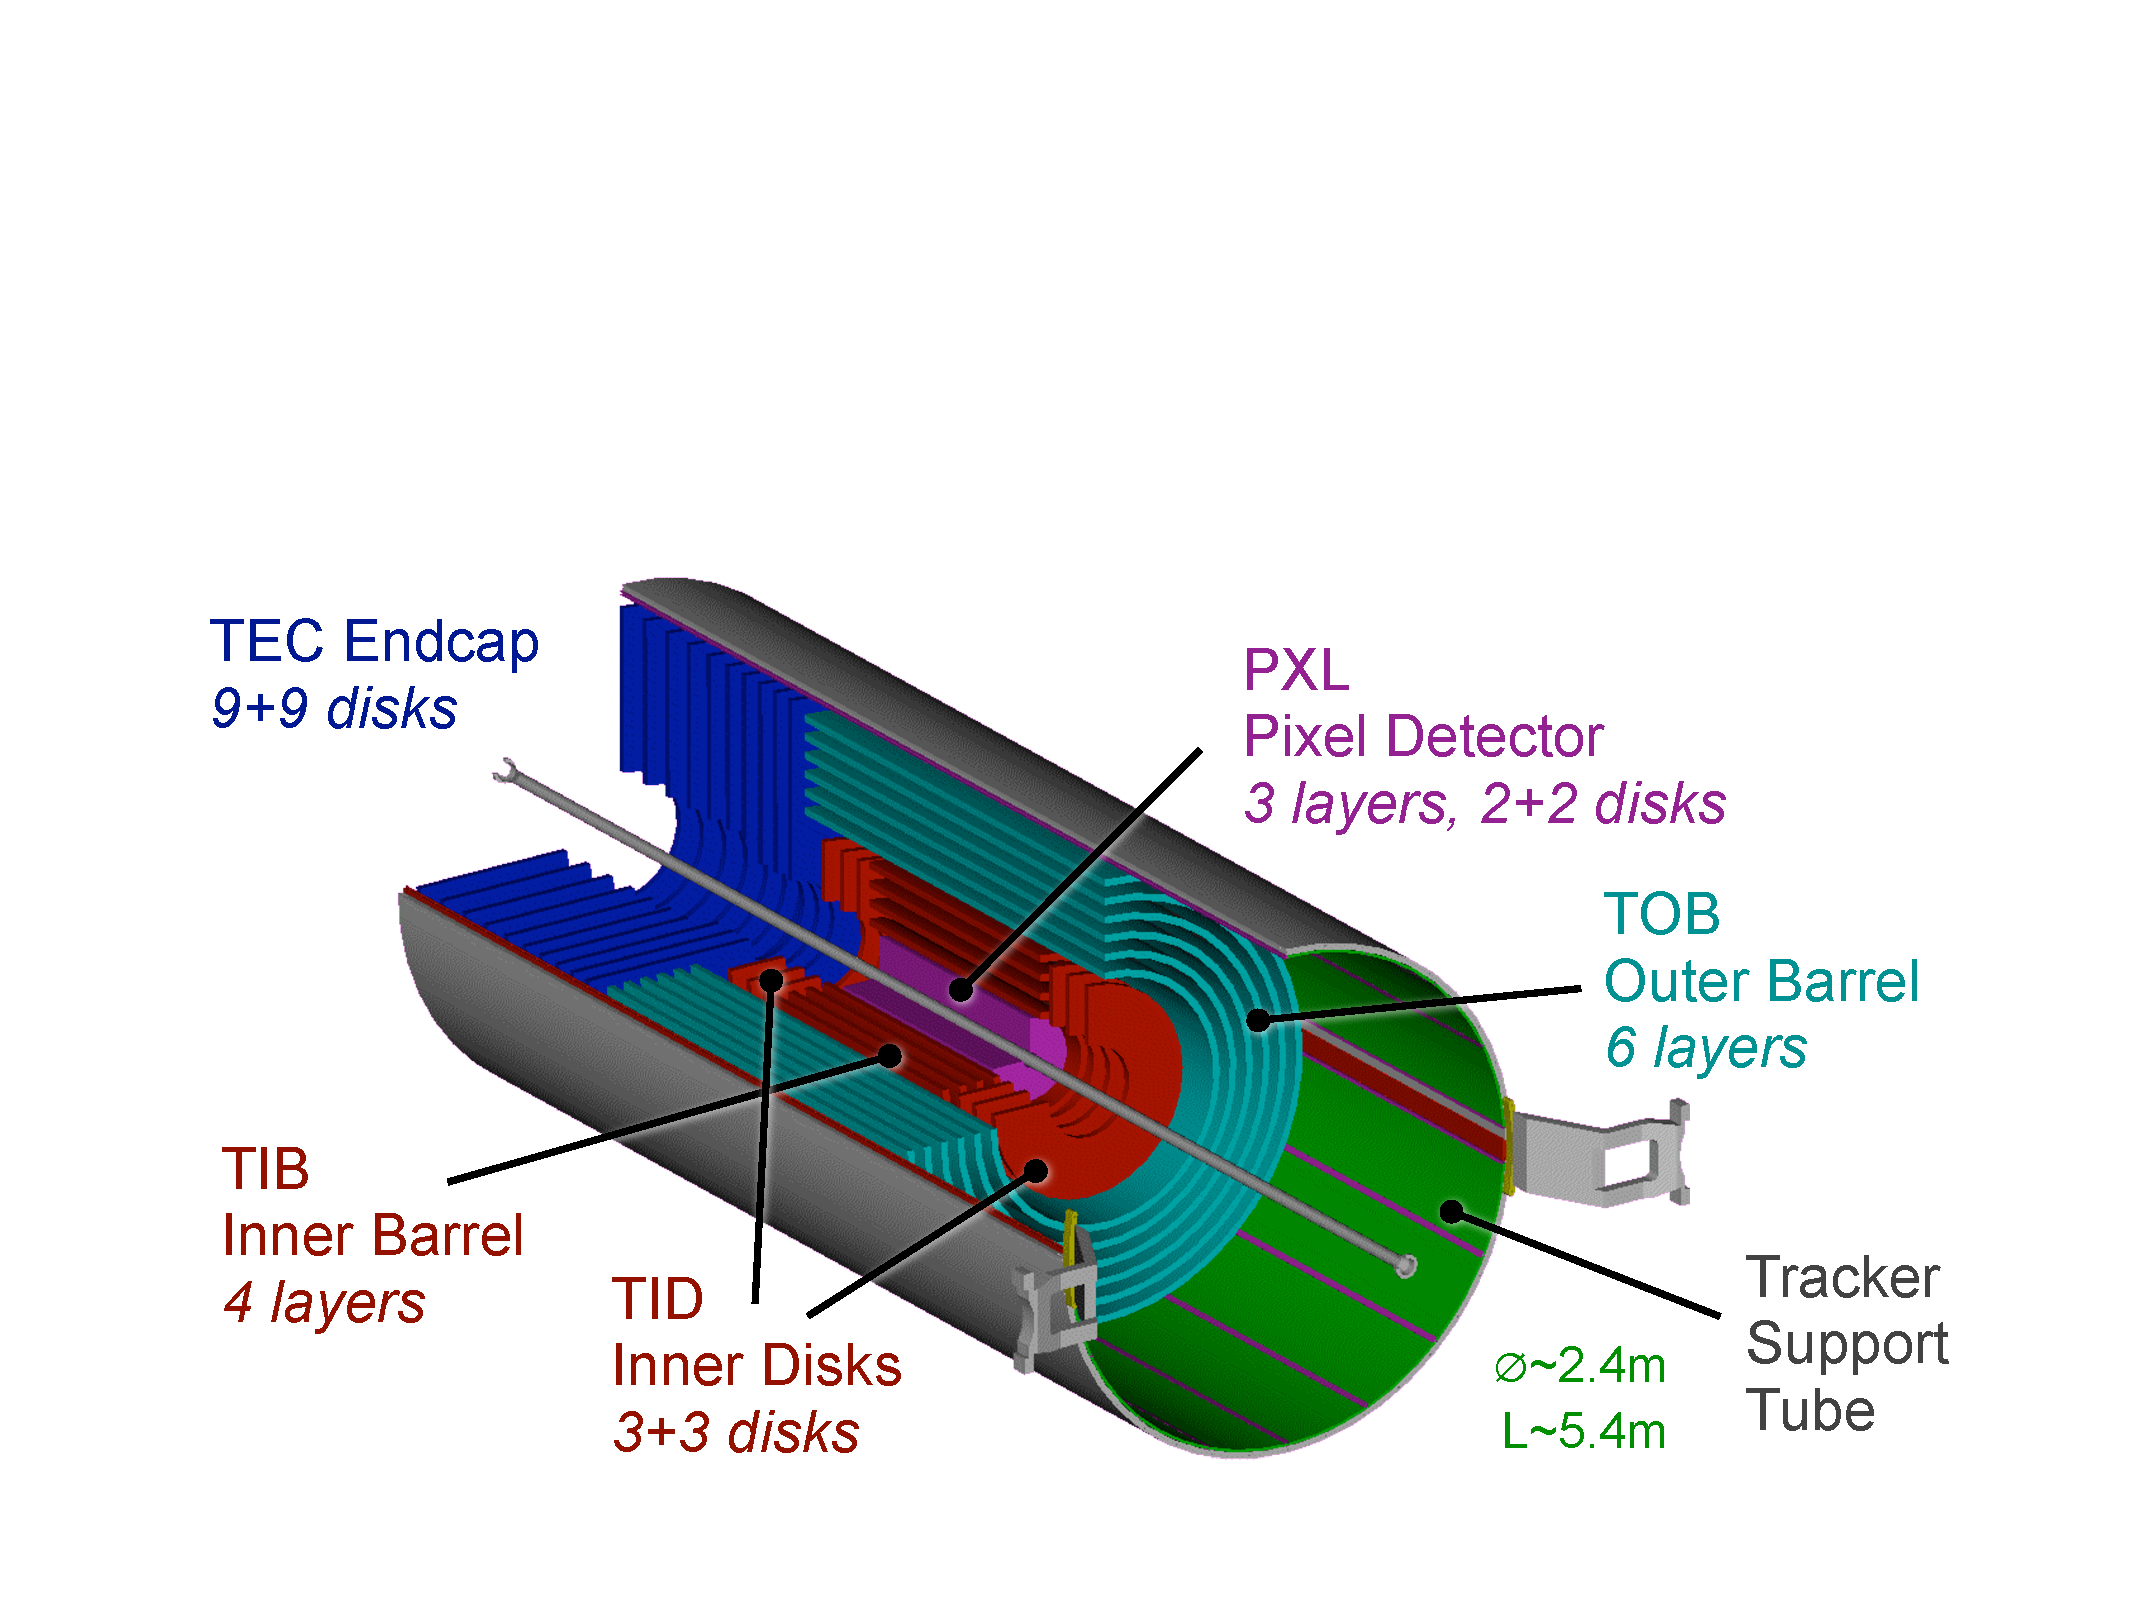
\includegraphics[width=0.45\textwidth]{Immagini/sketch.pdf}
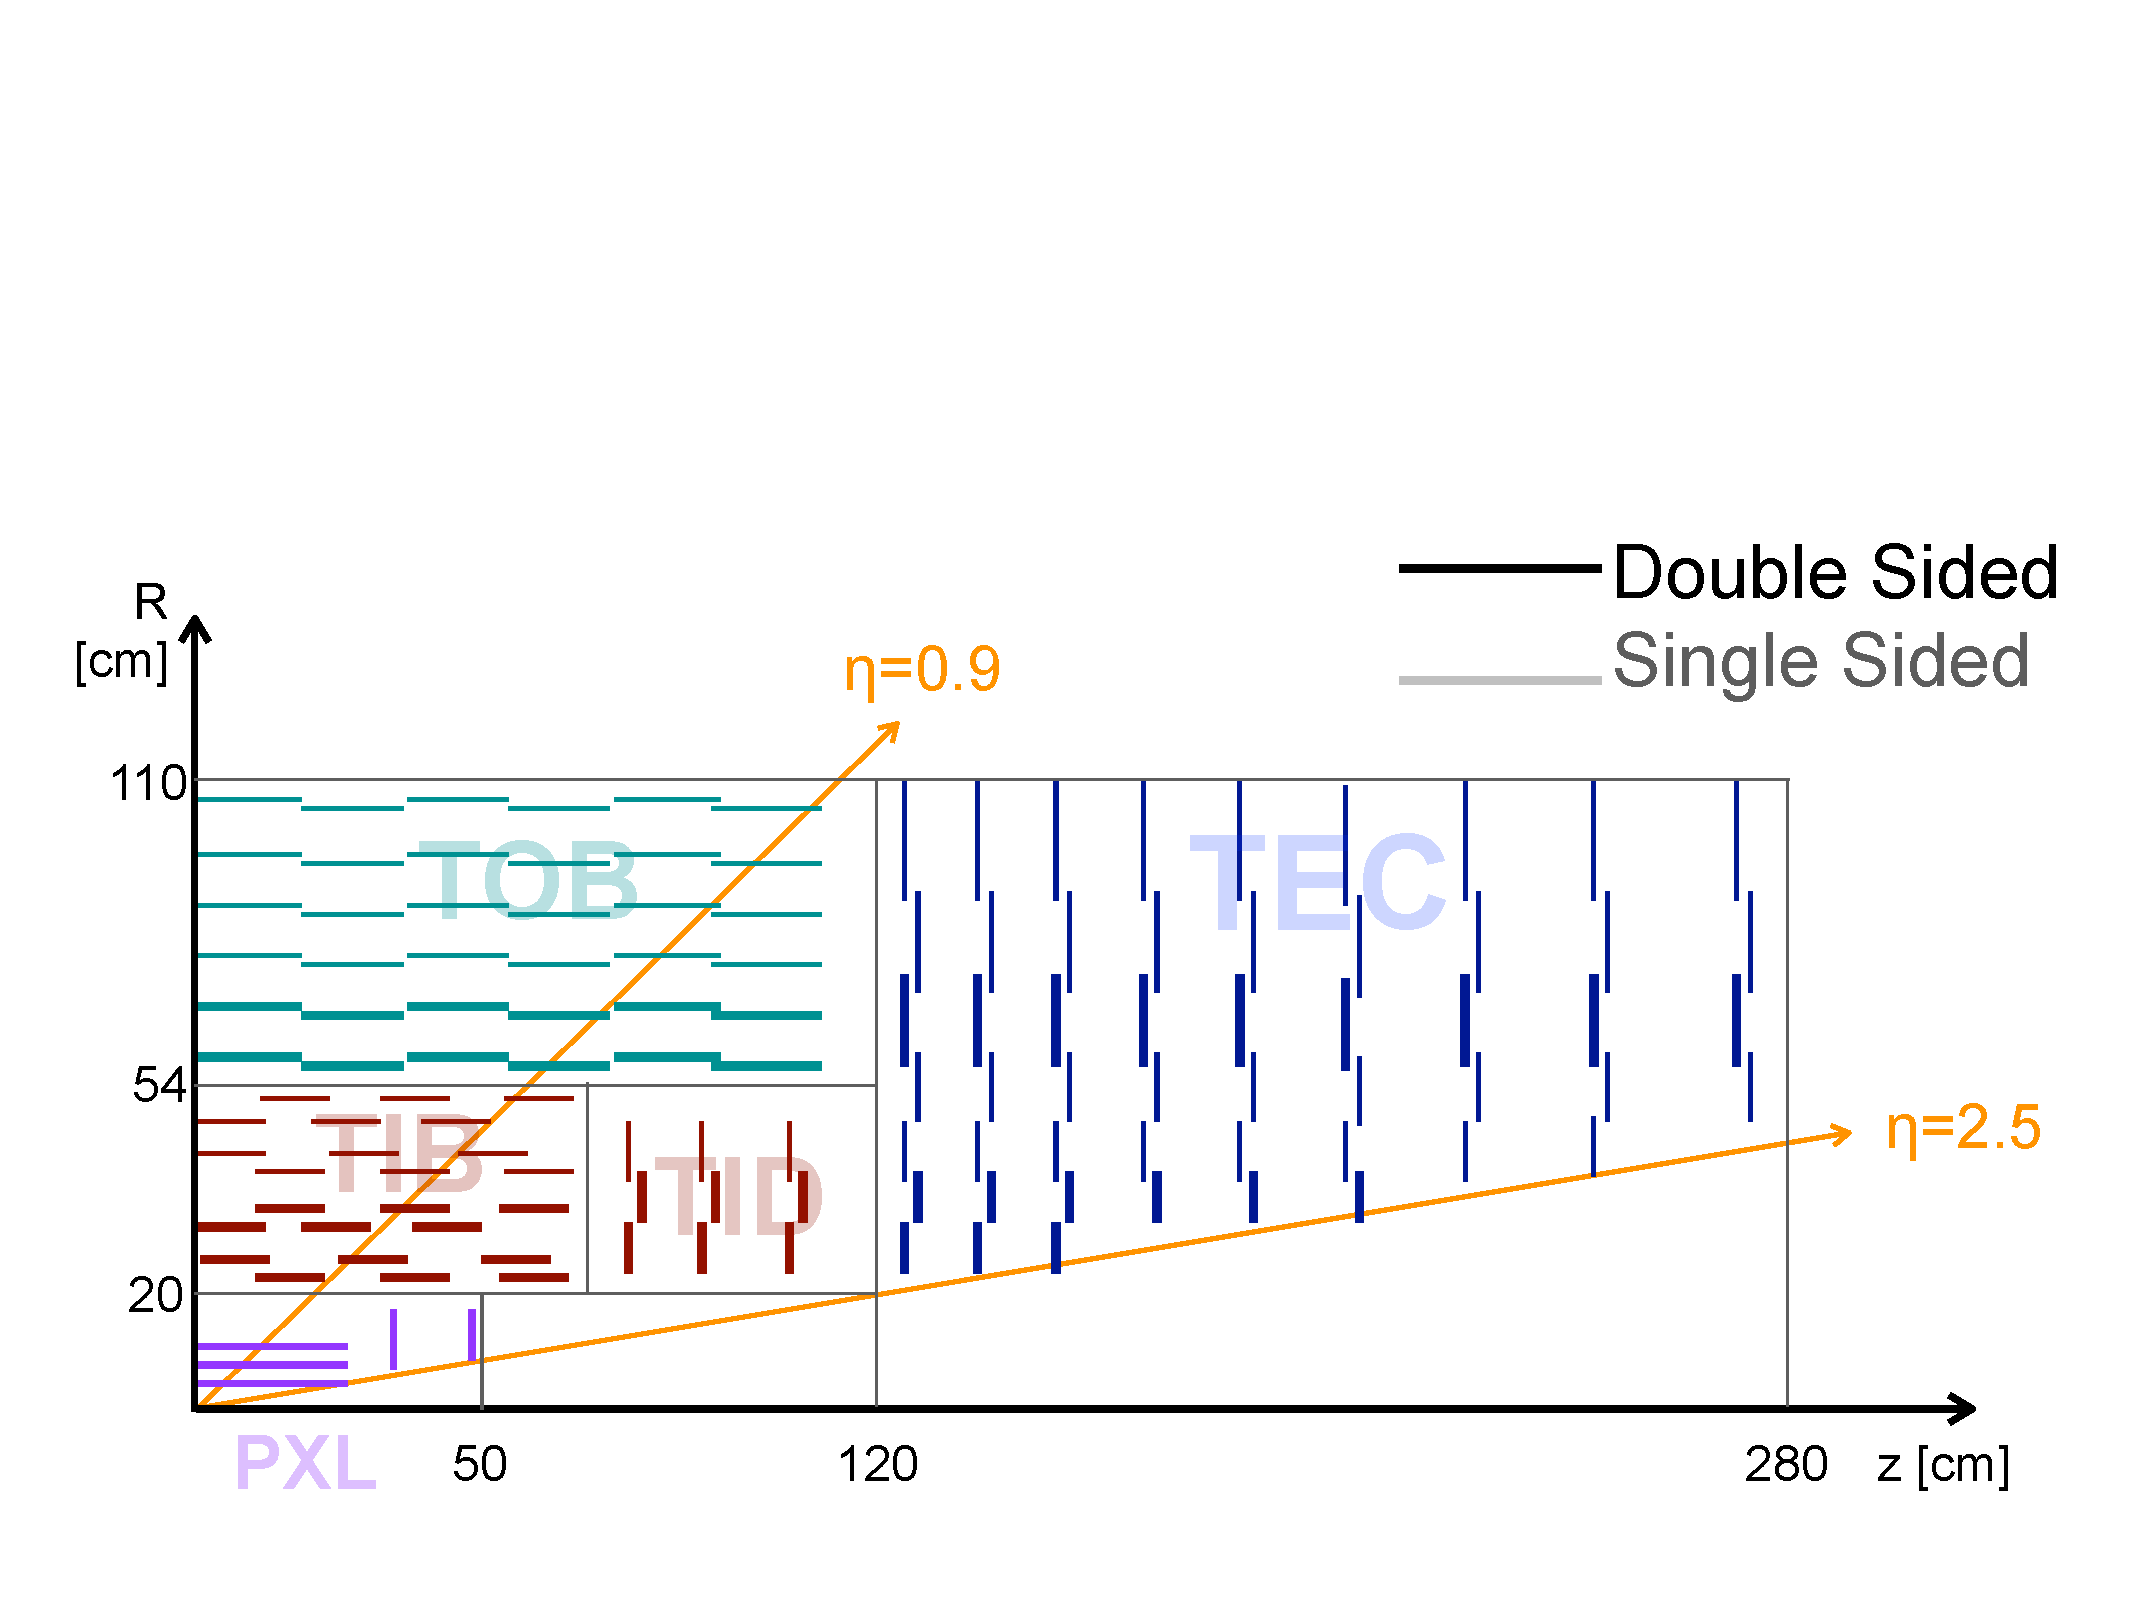
\includegraphics[width=0.95\textwidth]{Immagini/layout_rz.pdf}
\caption{Vista $Rz$ di un quadrante del tracciatore di CMS con il pixel detector di fase-0. Nella parte di rivelatore a strisce le linee massicce rappresentano i moduli stereo.}
\label{fig:CMSTk}
\end{figure}

Una vista di CMS durante l'istallazione del tracciatore \`e visibile in~Fig.~\ref{fig:CMS}.
\begin{figure}
\centering
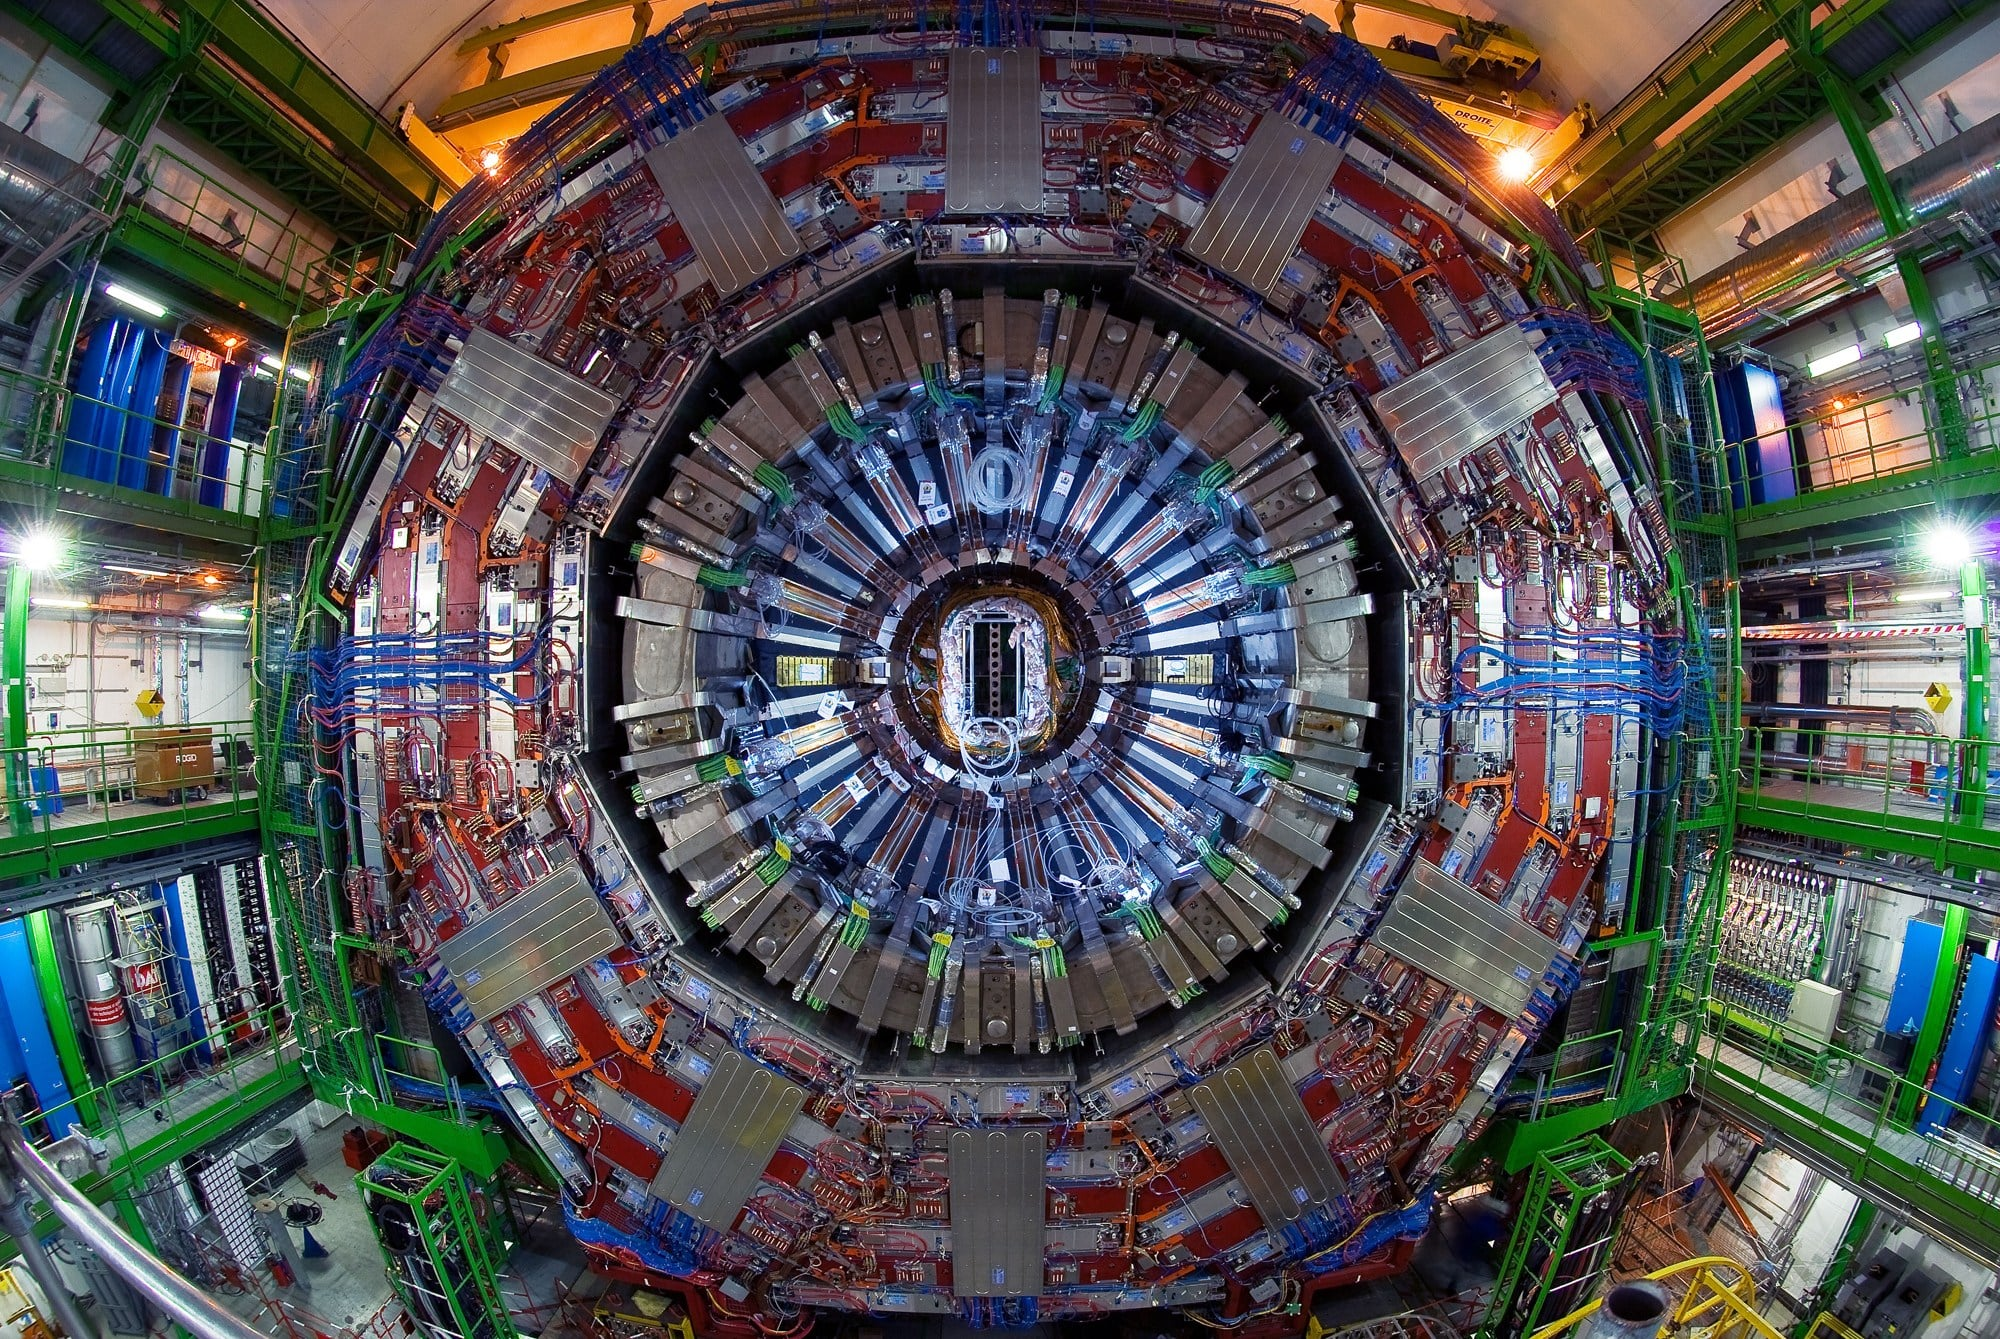
\includegraphics[scale=.2]{Immagini/CMS}
\caption{Vista frontale di CMS durante l'installazione del tracciatore.}
\label{fig:CMS}
\end{figure}

\begin{description}

\item[Il rivelatore a pixel.] Detto anche {\em rivelatore di vertice}, \`e il primo rivelatore che si incontra uscendo dal punto di collisione. CMS ha utilizzato una prima versione del rivelatore di pixel (detta di {\em fase-0}) fino al 2016. A partire dal 2017 \`e operativa una seconda versione evoluta e migliorata, detta di {\em fase-1}. Il rivelatore di vertice \`e fondamentale perch\'e, grazie alla bassa occupancy, fornisce alla ricostruzione le proto-tracce ({\em seeding}) da estrapolare verso l'esterno per l'individuazione dei segnali ({\em hit}) riconducibili alla medesima particella ({\em pattern recognition}) da cui sono poi estratti ({\em fitting}) i parametri della traccia. Contribuisce inoltre all'identificazione dei vertici primari e delle particelle a lunga vita media.
 
Il rivelatore a pixel di fase-0 era composto da una parte barrel di tre strati approssimativamente cilindrici e coassiali lunghi $\sim 53\cm$ e posizionati a $\sim 4.4\cm$, $\sim 7.3\cm$ e $\sim 10.2\cm$ in raggio. Ogni cilindro \`e composto da strutture di supporto e di raffreddamento per i moduli a pixel ({\em ladders}), ognuna contenente 8 moduli. Il rivelatore era completato in avanti da due dischi per lato fino a $z\sim\pm 46.5\cm$ per un totale di 1440 moduli, $1.06\m^2$ di silicio, 66M di canali. I sensori, di $250\um$ di spessore, sono segmentati in pixel di $100\times150\um^2$ tramite impiantazioni di tipo n$^+$-on-n mentre la giunzione \`e realizzata sulla faccia opposta del cristallo. Il segnale \`e letto da appositi chip di lettura ({\em Readout Chips} o ROC) connessi ai sensori tramite {\em bump bonding}. Il ROC \`e un ASIC ({\em Application Specific Integrated Circuit}), realizzato con tecnologia commerciale CMOS a $0.25\um$, e ospita una matrice di $52\times80$ canali. La risoluzione spaziale sulla posizione di passaggio della traccia \`e $10--15\um$.

Il rivelatore di pixel di fase-0, progettato per una luminosit\`a istantanea di $10^{34}\cm^{-2}\s^{-1}$ al picco, era afflitto da alcune limitazioni che si sono mano a mano manifestate con l'aumento della luminosit\`a istantanea e l'invecchiamento del rivelatore. Tra queste le principali sono: inefficienza dinamica in caso di alta occupancy e elevata frequenza di trigger dovute all'architettura del ROC, anche dell'ordine del 15\% negli strati pi\`u interni a $2\cdot10^{34}\cm^{-2}\s^{-1}$; peggiore ricostruzione delle tracce a causa della riduzione di qualit\`a del seeding a causa del fondo elevato dovuto al PU; danneggiamento da radiazione nei sensori che riduce il segnale di particella e, di conseguenza, la risoluzione spaziale.

Il rivelatore di pixel di fase-1 \`e concepito per superare queste limitazioni. Pur essendo simile alla precedente versione, \`e composto da quattro strati nella parte barrel rispettivamente di $\sim 3.0\cm$, $\sim 6.8\cm$, $\sim 10.2\cm$ e $\sim 16.0\cm$ di raggio. Gli endcap sono composti da tre dischi per lato fino a $z\sim\pm 51\cm$ per un totale di 1856 moduli, $1.95\m^2$ di silicio per 124M di canali. L'incremento dei punti di misura e il primo layer pi\`u vicino all'IP rende il seeding pi\`u robusto anche in presenza di PU. I sensori sono identici alla versione precedente ma completamente nuovi e non danneggiati. L'architettura della nuova generazione di ROC utilizzati permette di ridurre drasticamente l'inefficienza dinamica per le luminosit\`a istantanee previste fino a LS3. 

La geometria delle due versioni del rivelatore a pixel di CMS \`e comparativamente visibile in~Fig.\ref{fig:PXLph0ph1}.
\begin{figure}
\centering
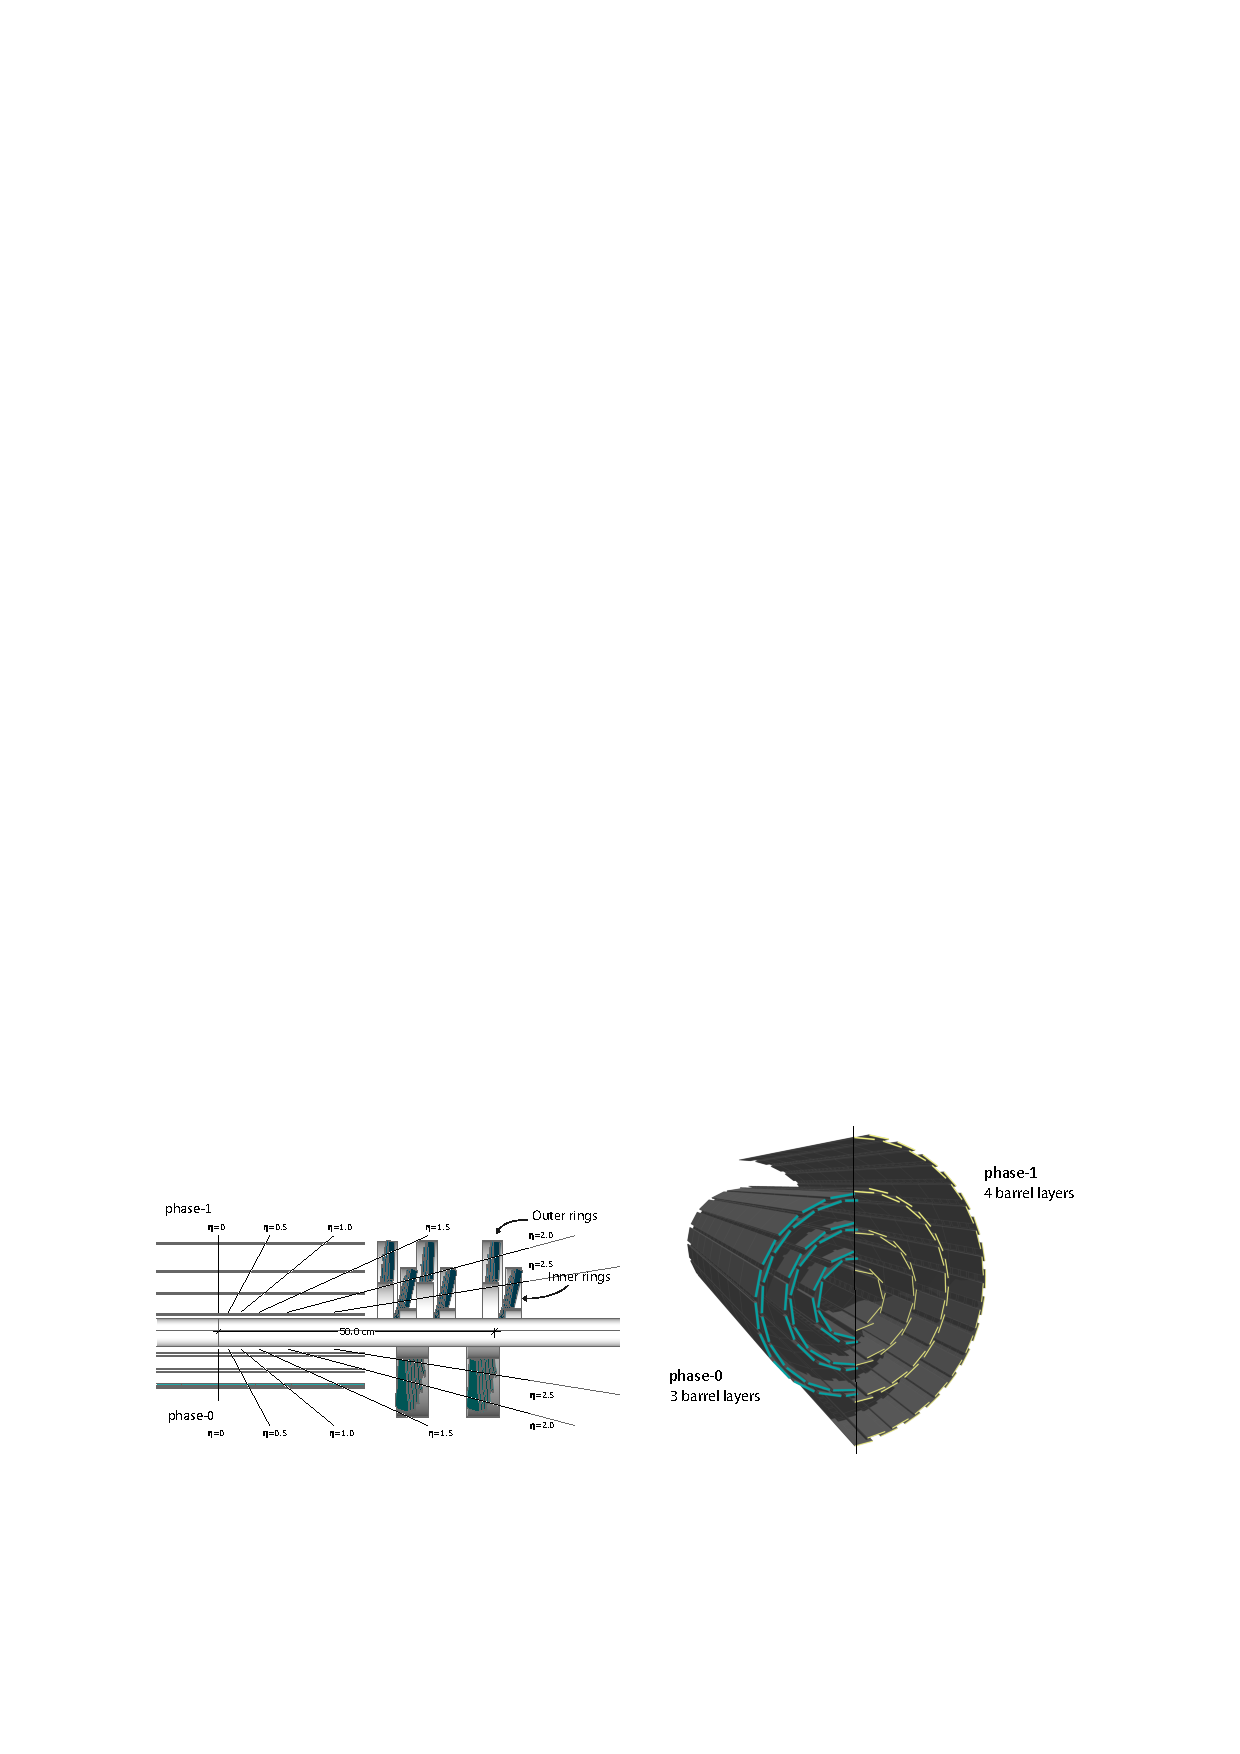
\includegraphics[width=0.98\textwidth]{Immagini/PXLph0ph1.pdf}
\caption{Rappresentazione schematica della geometria delle due versioni del rivelatore a pixel di CMS nella vista $Rz$ e in una vista prospettica della parte barrel.}
\label{fig:PXLph0ph1}
\end{figure}

\item[Il rivelatore a microstrip.] L'attuale rivelatore a microstrip copre la regione compresa tra $R\sim 20\cm$ e $R\sim 110\cm$ rispetto all'asse dei fasci. Come rappresentato in Fig.~\ref{fig:CMSTk}, il barrel ($|z|<110\cm$) \`e suddiviso in una parte interna di quattro strati ({\em Tracker Inner Barrel}, TIB) e di una parte esterna di sei strati ({\em Tracker Outer Barrel}, TOB). Il TIB \`e integrato da due endcap di tre dischi ciascuno ({\em Tracker Inner Disks}, TID). I volumi in avanti ($120\cm < |z| < 280\cm$) sono attrezzati con nove dischi per lato ({\em Tracker End-Cap}, TEC) che garantiscono un'accettanza fino a $|\eta|<2.5$. Complessivamente il tracciatore occupa un volume di $\sim 23\m^3$ ed \`e il rivelatore a silicio pi\`u grande mai costruito dato che \`e composto da $\sim 15000$ moduli per un totale di $198\m^2$ di silicio e $\sim 9.6M$ di canali con lettura ottica.

Pur nelle diverse tipologie e dimensioni, ciascun modulo \`e costituito da un sensore a strisce, ottenute con impiantazione di tipo p$^+$ su substrato di tipo n, e dalla relativa elettronica di prossimit\`a. La lunghezza e il passo delle strisce e lo spessore del silicio dipendeno dalla collocazione del modulo: internamente, dove \`e richiesta una maggiore granularit\`a, le strisce sono lunghe $\sim 12\cm$ con un passo compreso tra $80\um$ e $120\um$ e lo spessore \`e $320\um$; esternamente le strisce sono lunghe $\sim 20\cm$ con un passo compreso tra $120\um$ e $\sim 200\um$ e lo spessore di $500\um$ garantisce un segnale maggiore che compensa il maggior carico capacitivo dovuto alla lunghezza delle strisce. I moduli delle strutture a disco hanno sensori con forma trapezoidale con le strisce disposte radialmente.

Alcuni degli strati e porzioni dei dischi, particolarmente nelle regioni pi\`u interne, sono equipaggiati con speciali moduli doppia-faccia (rappresentanti da linee massicce in~Fig.\ref{CMSTk}), che forniscono un'accurata misura tridimensionale della posizione di passaggio della particella carica, ottenuti accoppiando due sensori introducendo un angolo relativo pari a 100mrad tra le strisce. 
\end{description}

I rivelatori a silicio hanno bisogno di una o pi\`u alimentazioni ad alta corrente per il funzionamento dell'elettronica, tipicamente nel range tra 1 e $2\V$ e genericamente indicate con ``basse tensioni'' (LV), e della tensione per la polarizzazione dei silici stessi che pu\`o raggiungere anche 1000V (``alta tensione'' o HV). Una breve descrizione del sistema di alimentazione LV dell'attuale tracciatore di CMS \`e utile per contestualizzare il presente lavoro di tesi. CMS utilizza un complesso sistema modulare basato su $\sim 2000$ unit\`a di alimentazione ({\em power supply units}, PSU), installate nella caverna dove si trova CMS, che forniscono ai moduli le tesioni necessarie tramite cavi a bassa impedenza, lunghi diverse decine di metri,
%(LIC, da Low Impedance Cable)
appositamente sviluppati. Lo schema adottato \`e quello di alimentazione diretta, ovvero non ci sono stadi intermedi di conversione di tensione, e la tensioni sono controllate con sonde ad alta impedenza in prossimit\`a del carico ({\em sensing}) e questo consente di regolare le tensioni di alimentazione sull’elettronica di readout del rivelatore compensando le cadute sui cavi e gestendo i transienti dovuti alle variazioni repentine di assorbimento derivanti dall'attivit\`a dell'apparato.

Una evidente conseguenza di questo approccio \`e l'impatto che i cavi di alimentazione hanno sul materiale passivo del tracciatore che deve essere tenuto al minimo per non degradare le prestazioni dell'apparato a causa di scattering multiplo, perdita di energia, conversioni di fotone e interazioni nucleari.  
Date le alte potenze in gioco, la massa necessaria per i cavi di alimentazione per limitare la caduta di tensione non \`e trascurabile nonostante si utilizzino, ove possibile, anche cavi in leghe di alluminio per mitigare il problema.

Il rivelatore a pixel di fase-0 necessita di due tensioni LV, $+2.5\V$ e $+1.75\V$ per una potenza media erogata dagli alimentatori di $\sim 7kW$. Il tracciatore a microstrisce necessita di due tensioni LV, $+2.5\V$ e $+1.25\V$ per una potenza media che il sistema di alimentazione fornisce \`e pari a $\sim 70\kW$. Per entrambi i sottosistemi approssimativamente la met\`a della potenza viene dissipata nei cavi.

Il rivelatore a pixel di fase-1, pur abbisognando di tensioni analoghe al suo predecessore, ha abbandonato l'approccio di alimentazione diretta introducendo uno stadio di conversione vicino al carico ({\em Point of Load, POL, conversion}) basato su convertitori DC/DC che generano le tensioni necessarie a partire da una tensione intermedia ($\sim 8-12\V$) fornita dagli alimentatori. I convertitori DC/DC sono molto efficienti sfruttando la tecnologia switching per la conversione di tensione ma necessitano di un'induttore che limita la miniaturizzazione di questo componente. Grazie al trasferimento di potenza effettuato in gran parte a tensione intermedia, la potenza erogata dagli alimentatori per il pixel di fase-0 \`e di circa $5\kW$ di cui solo il 25\% \`e dissipato nei cavi.

A titolo di esempio, in Fig.~\ref{fig:CMSTkMB} (sinistra), \`e mostrato il profilo in funzione di $\eta$ del materiale passivo del tracciatore (espresso in lughezze di radiazione), con il pixel di fase-0 ({\bf 2014 JINST 9 P10009 (1405.6569)}). Il miglioramento introdotto, anche rispetto al materiale, dal pixel di fase-1 rispetto al suo predecessore \`e mostrato in Fig.~\ref{fig:CMSTkMB} (destra) ({\bf TDR fase-1}). Pur tuttavia l'ammontare del materiale passivo dell'attuale tracciatore di CMS pu\`o essere considerato uno degli aspetti suscettibili di miglioramento.
\begin{figure}
\centering
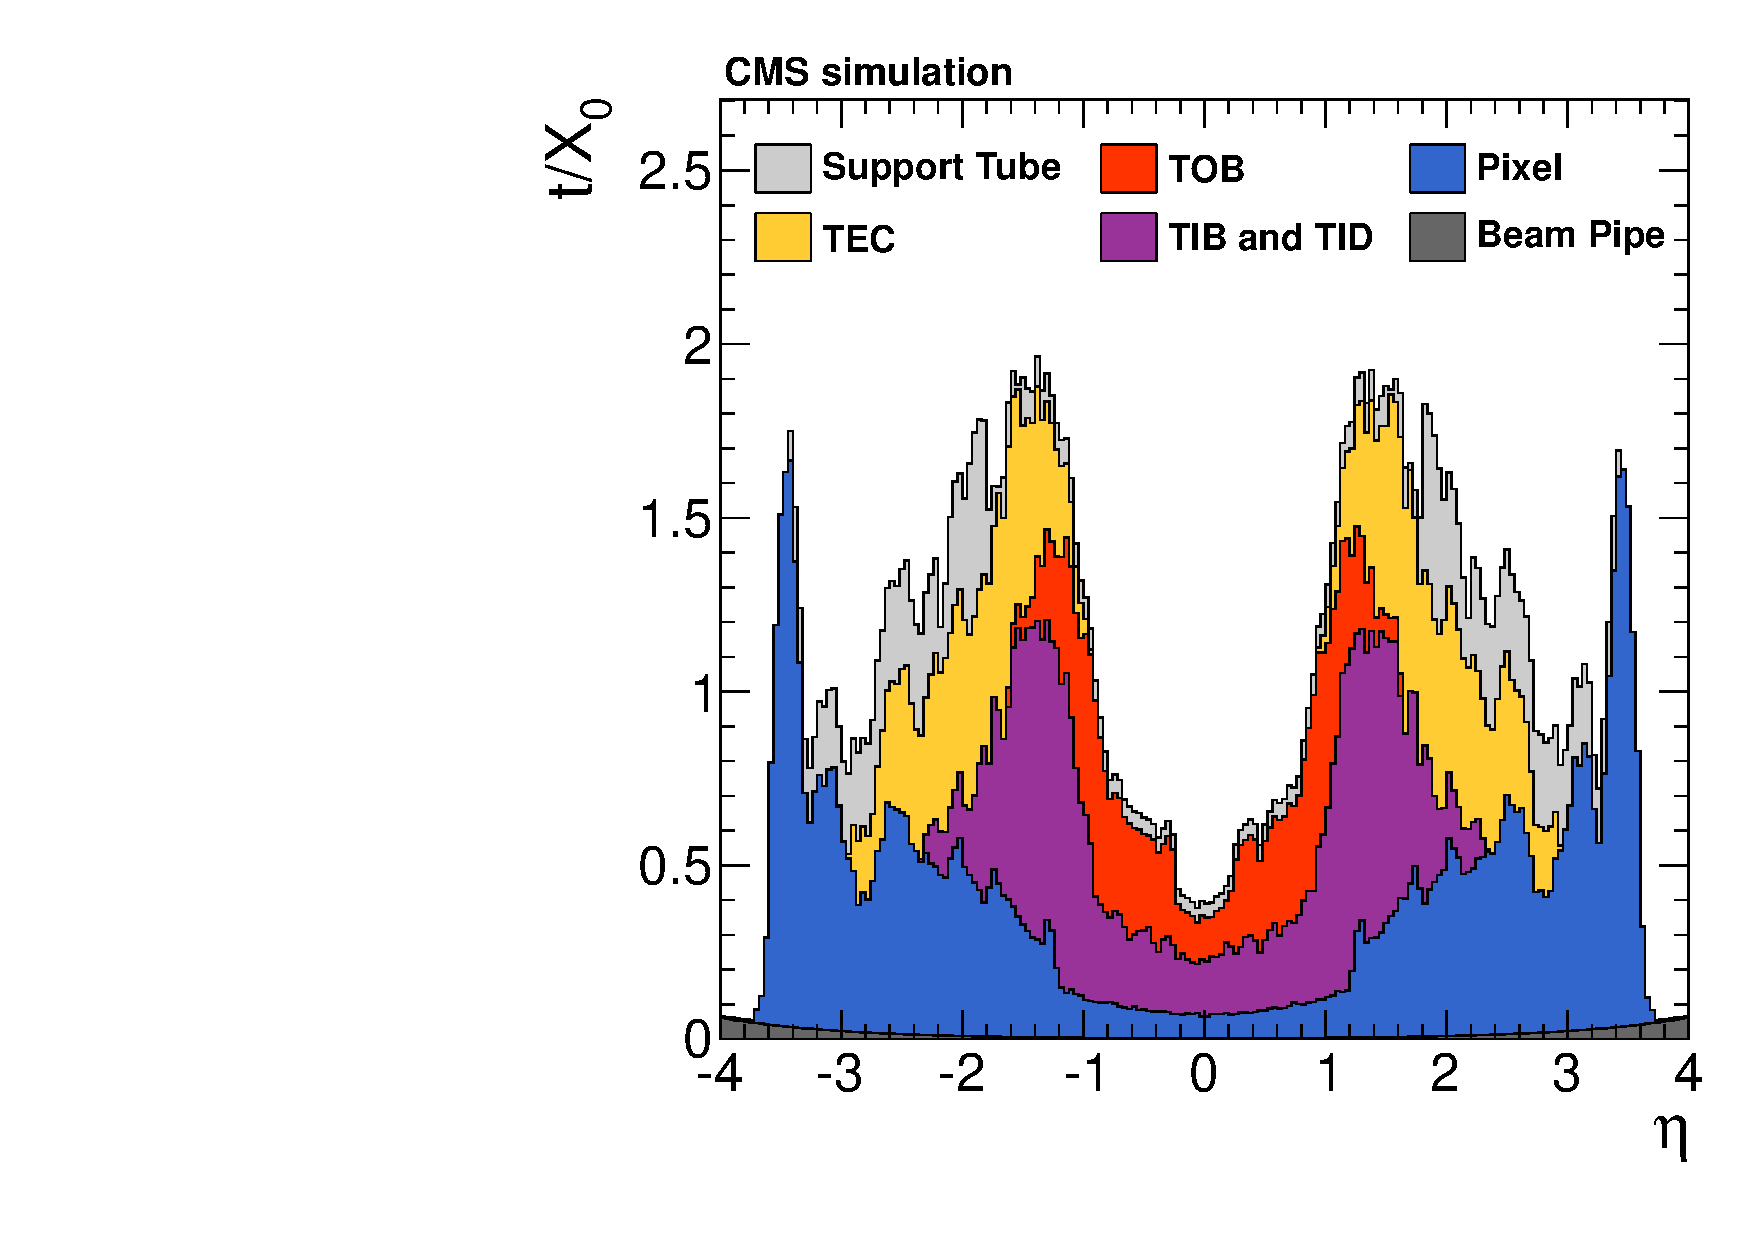
\includegraphics[width=0.42\textwidth]{Immagini/Tracker_SubDetectors_x_vs_eta.pdf}
\hfill
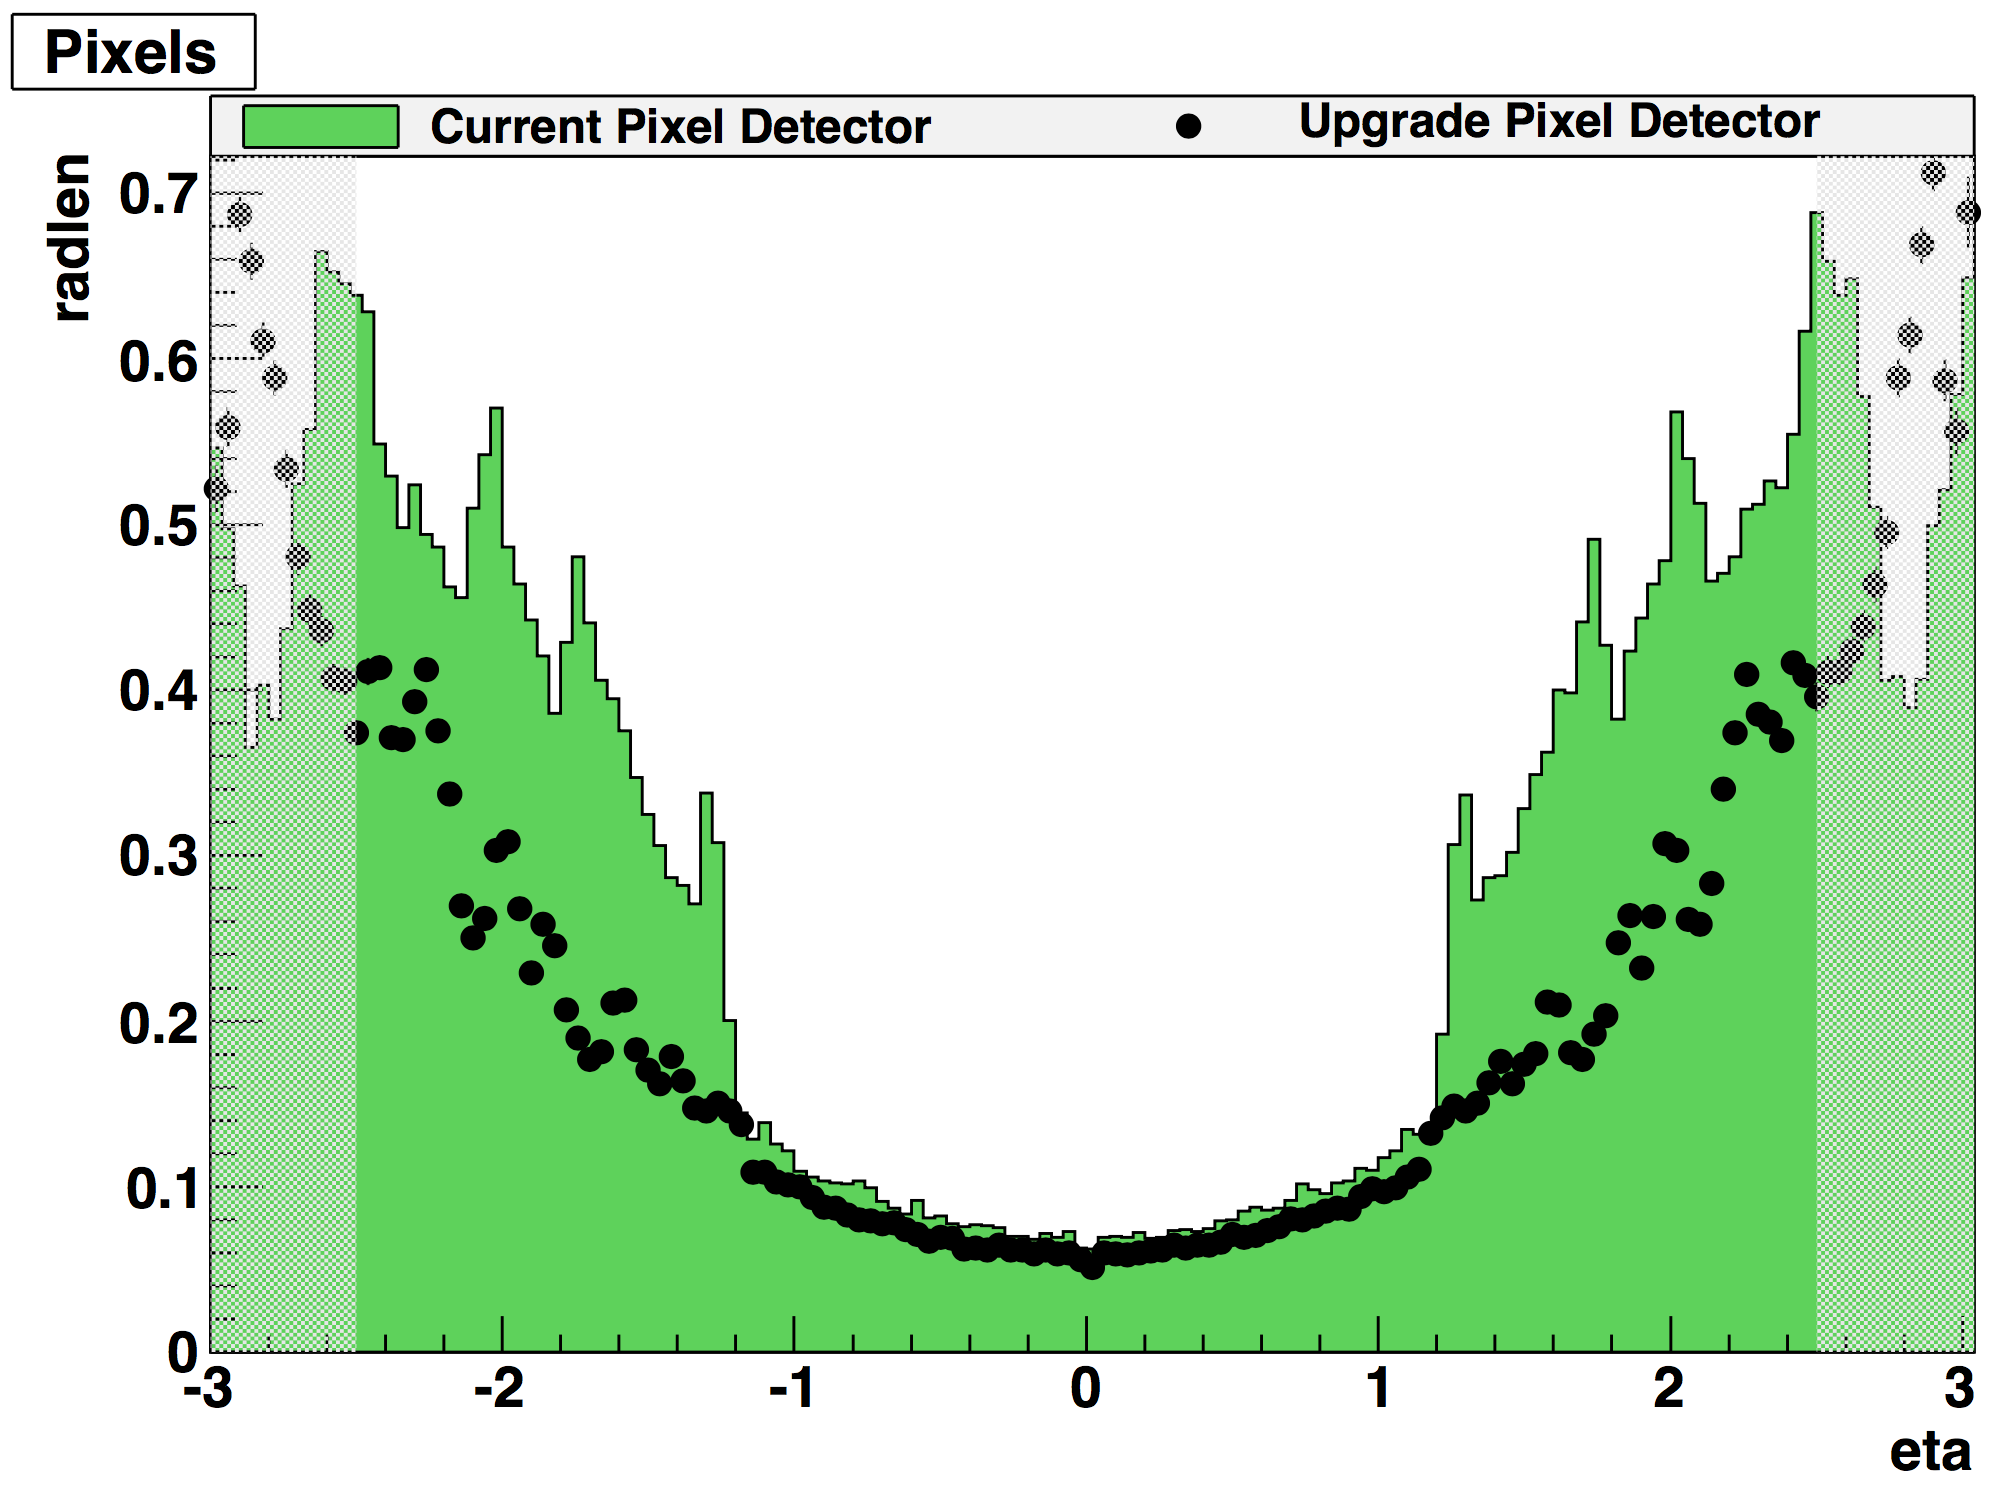
\includegraphics[width=0.53\textwidth]{Immagini/CMSPXL_ph0ph1_MB.PNG}
\caption{Sinistra: spessore totale $t$ del tracciatore di CMS con il pixel di fase-0 in unit\`a di lunghezza di radiazione $X_0$ in funzione di $\eta$. Destra: lo spessore in unit\`a di $X_0$ in funzione di $\eta$ del pixel di fase-0 (profilo verde), rispetto al pixel di fase-1 (punti); la regione ombreggiata rappresenta le regioni al di fuori dell'accettanza del tracciatore.}
\label{fig:CMSTkMB}
\end{figure}


\section{Il Tracciatore di CMS per HL-LHC}

Per HL-LHC il tracciatore di CMS deve essere completamente sostituito sia a causa del danneggiamento da radiazione e del peggioramento delle prestazioni a cui sarebbe altrimenti sottoposto, sia per avere un apparato compatibile con condizioni operative molto pi\`u esigenti (ref. CMS Collaboration, “Technical Proposal for the Phase-II Upgrade of the CMS Detector”, CERN-LHCC-2015-010, LHCC-P-008, CMS-TDR-15-02 (2015); CMS Collaboration, “CMS Phase II Upgrade Scope Document”, Technical Report CERN-LHCC-2015-019, LHCC-G-165, CERN, Geneva, 2015). 

Il danneggiamento da radiazione accumulato dei sensori a pixel riduce la collezione di carica e, a lungo termine, la risoluzione e l'efficienza. 
Per quanto riguarda i sensori a strisce, l'effetto pi\`u evidente \`e l'aumento della tensione HV di polarizzazione per svuotare completamente il sensore e della corrente di buio. Di conseguenza gran parte dei moduli doppia-faccia non potrebbero pi\`u funzionare gi\`a per $1000ifb$ di luminosit\`a integrata. Le prestazioni risulterebbero gravemente degradate tanto da compromettere inaccettabilmente il programma sperimentale di CMS e questo senza tener conto delle limitazioni in termini di latenza e di portata di trasferimento dei dati ({\em readout bandwidth}).

Nonostante i previsti miglioramenti, il trigger di Livello 1 basato esclusivamente sulle camere a muoni e sull'informazione calorimetrica, a causa della limitata risoluzione, non sarebbe in grado di filtrare gli eventi per la contaminazione irriducibile dei fondi indotti dal PU e dall'elevato numero di interazioni per unit\`a di tempo. Per aumentare la risoluzione e quindi il potere di reiezione del fondo, come mostrato in~Fig.~\ref{fig:CMSTkL1} per un rilevante esempio, il tracciatore \`e chiamato a fornire informazione al sistema di trigger di L1 nella forma di tracce ad alto impulso trasverso ({\em track trigger}).
\begin{figure}
\centering
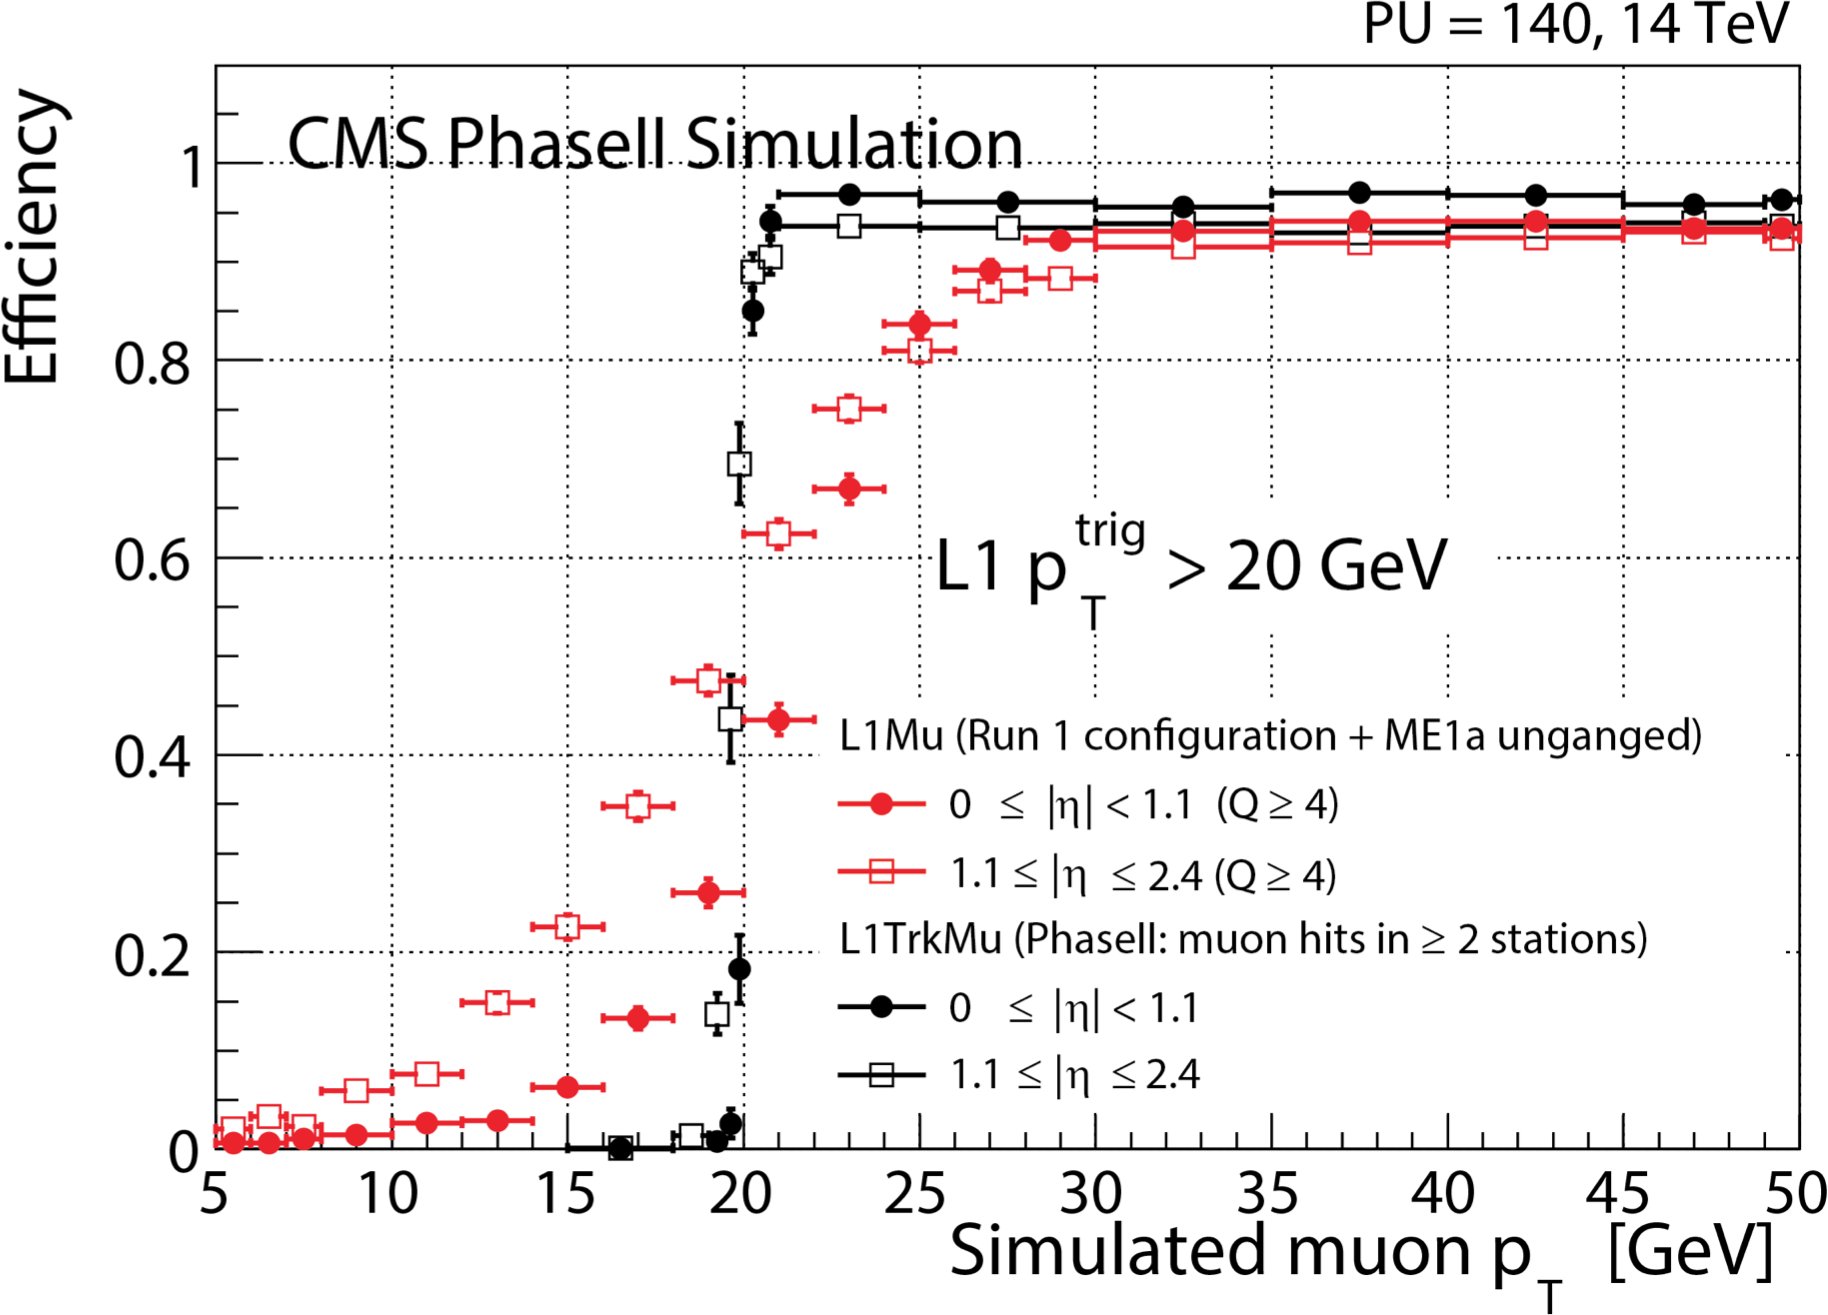
\includegraphics[width=0.45\textwidth]{Immagini/CMSTkL1_res.PNG}
\hfill
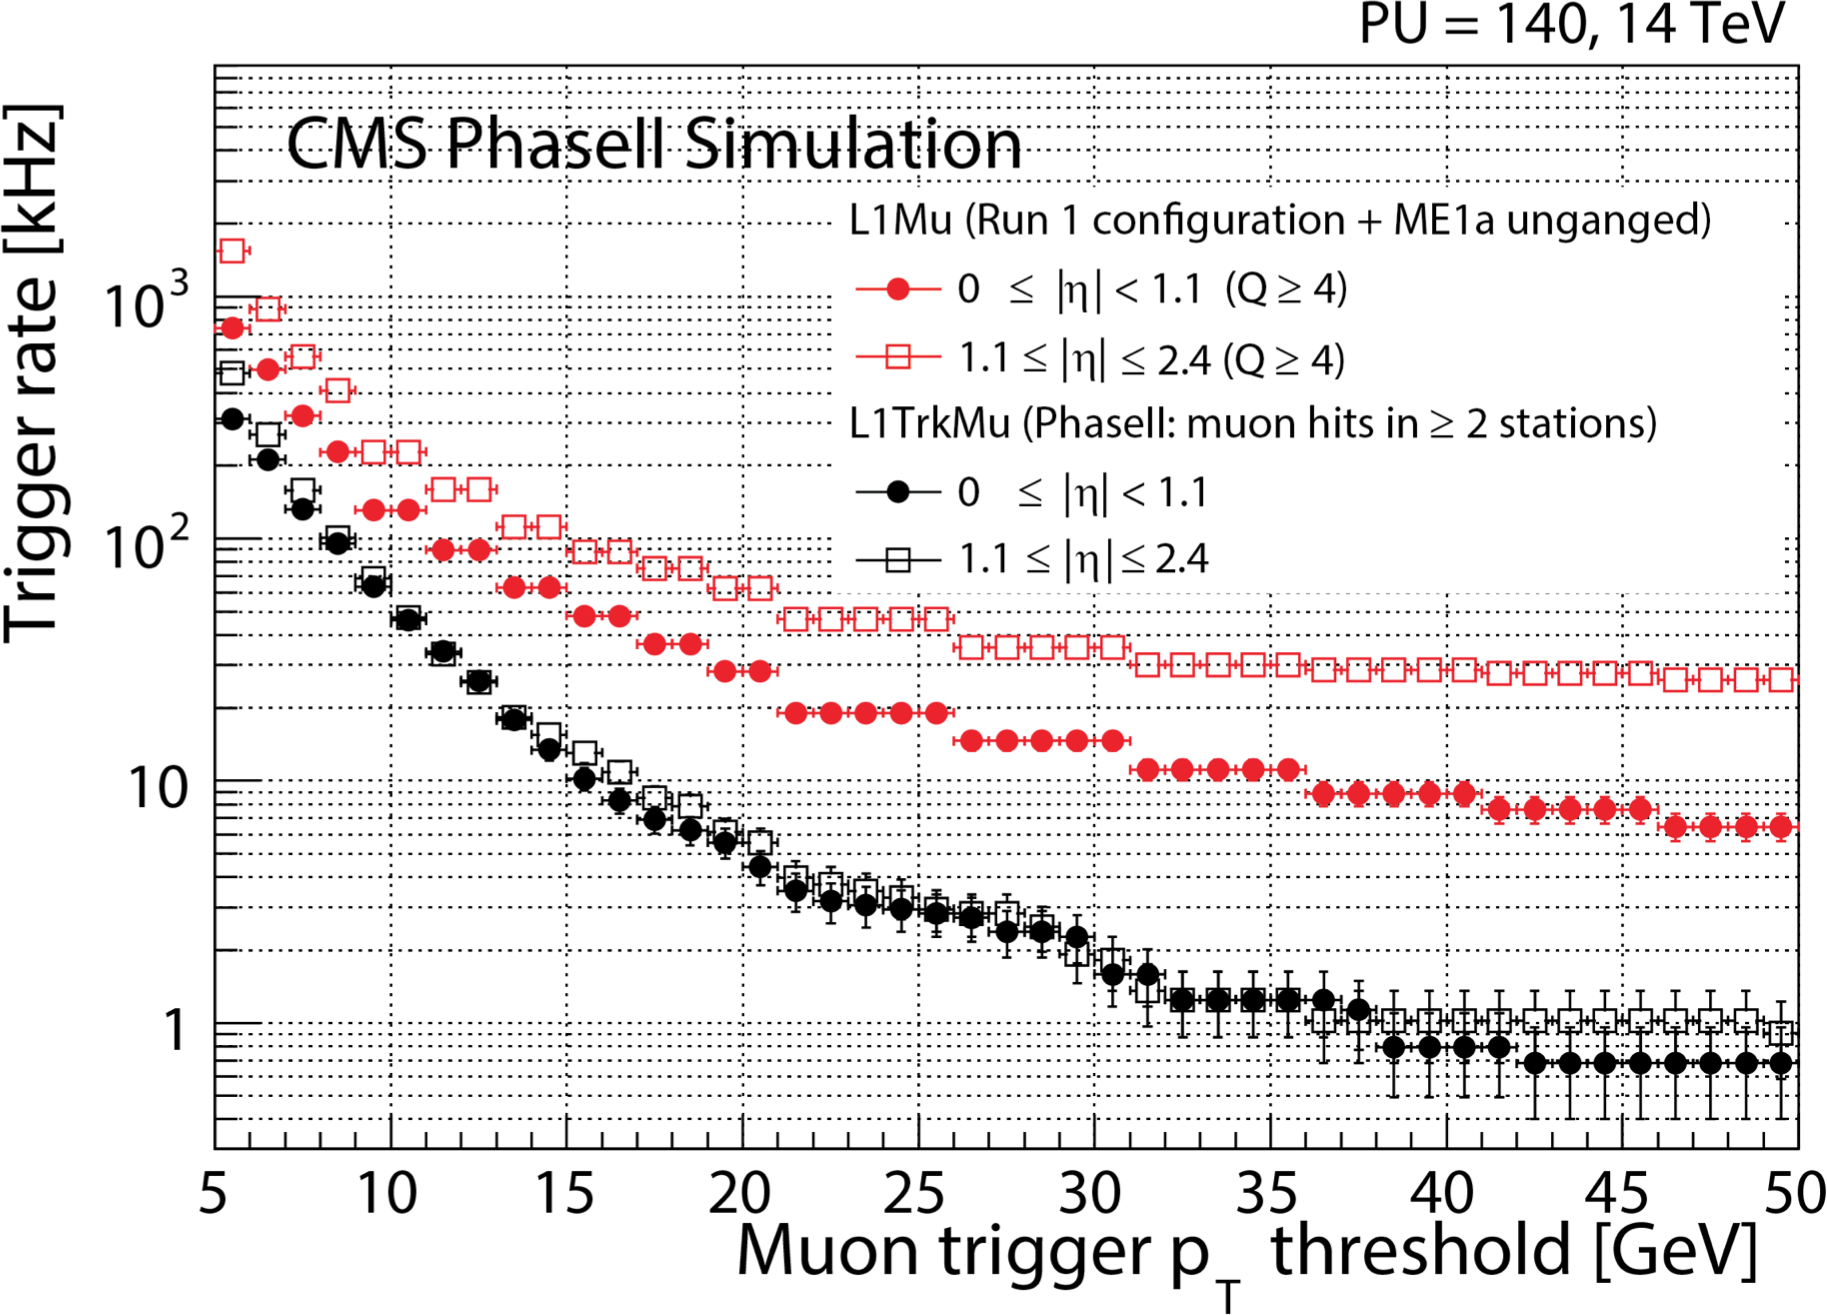
\includegraphics[width=0.45\textwidth]{Immagini/CMSTkL1_rate.PNG}
\caption{Sinistra: efficienza del trigger L1 di singolo muone con soglia a $20\GeV$, per due ambiti di $|\eta|$, in funzione del $\pt$ generato per l'algoritmo basato esclusivamente sulle camere a muoni (simboli rossi) e nel caso in cui si aggiunga l'associazione con una traccia (simboli neri). Destra: frequenza media in funzione della sogllia in $\pt$ per i due algoritmi di trigger sopra descritti in due diversi ambiti di $|\eta|$.}
\label{fig:CMSTkL1}
\end{figure}

La geometria concepita per il tracciatore di CMS per HL-LHC o di fase-2 \`e mostrata in~Fig.~\ref{fig:TkLayoutPhaseII}. Analogamente al tracciatore attuale, il Tracciatore per HL-LHC consister\`a di due sottoapparati. La parte interna o {\em Inner Tracker} (IT), basata su rivelatori a pixel organizzati in 4 strati nel barrel e 12+12 dischi endcap, equipaggia il volume vicino alla beam pipe corrispondente a $R<20\cm$ fino a $|z|<160\cm$ e $R<30\cm$ per $160\cm<|z|<270\cm$. La parte esterna o {\em Outer Tracker} (OT), basato su rivelatori a strisce a macro-pixel organizzati in 6 strati barrel e 5+5 dischi endcap, equipaggia il volume rimanente ($R<120\cm$, $|z|<270\cm$).
\begin{figure}
\centering
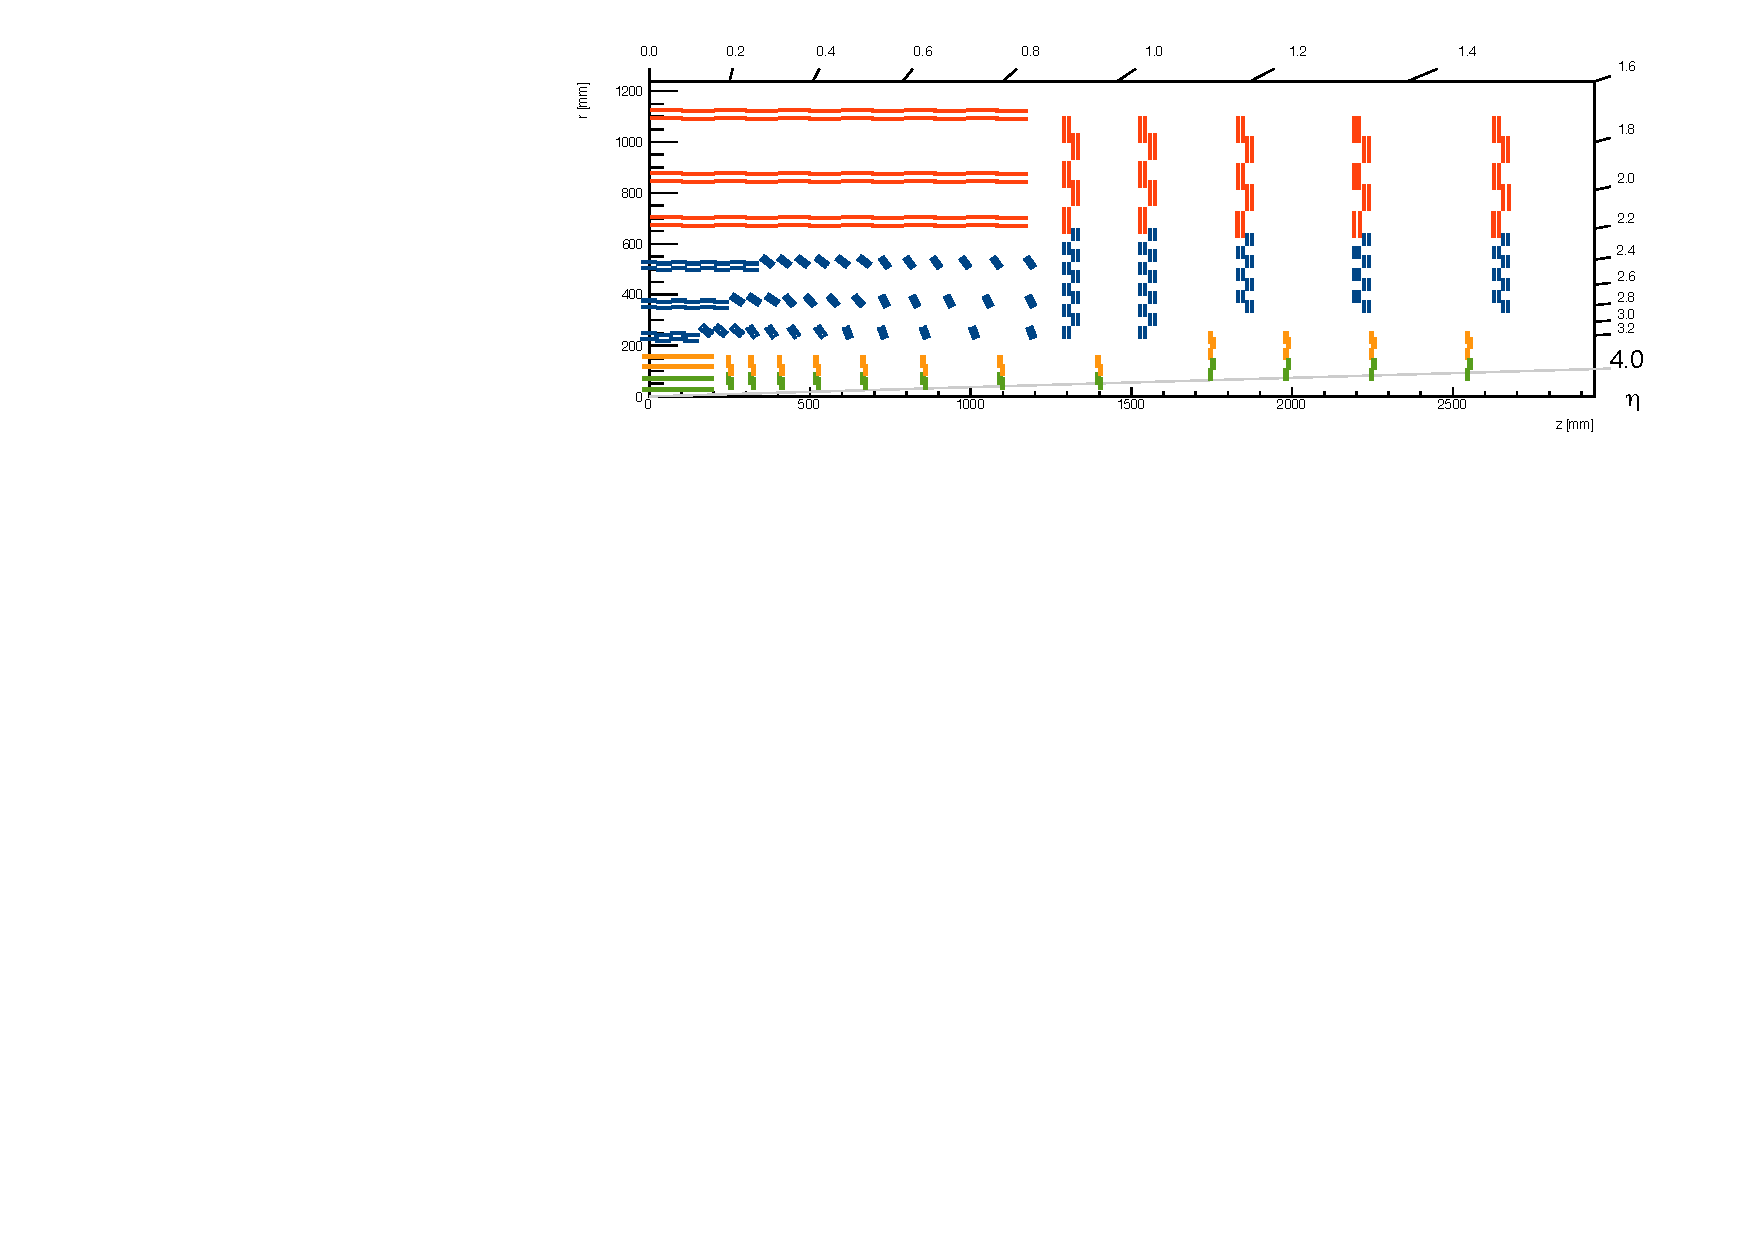
\includegraphics[width=0.99\textwidth]{Immagini/fullLayout000.pdf}
\caption{Geometria di un quadrante del tracciatore per HL-LHC nella vista $Rz$. L'Outer Tracker \`e rappresentato dai segmenti blu e rossi dei moduli di tipo PS e 2S rispettivamente; l'Inner Tracker a pixel \`e rappresentato dai segmenti verdi e gialli dei moduli 1x2 e 2x2, rispettivamente.}
\label{fig:TkLayoutPhaseII}
\end{figure}

Questa geometria e le altre scelte progettuali, descritte pi\`u avanti, derivano dall'esigenza di soddisfare i seguenti requisiti, schematicamente riassunti:
\begin{itemize}
% The general requirements for the Tracker upgrade are:
\item tolleranza alla radiazione e bassa temperatura di funzionamento ($-20\degrees$C) affinch\'e il tracciatore sia operativo fino a $3000\ifb$ (con appropriati per contemplare i $4500\ifb$ nello scenario a pi\`u alta luminosit\`a istantanea);
\item maggiore granulari\`a rispetto al tracciatore attuale per limitare l'occupancy a O(0.1\%) e O(1\%) per IT e OT, rispettivamente, e una geometria ottimizzata per una solida ed efficace pattern recognition; 
\item ottimizzazione del materiale passivo per minimizzarne gli effetti spuri (multiple scattering, bremsstrahlung, interazioni nucleari e conversione di fotoni);
\item track trigger per contribuire al trigger di Livello 1;
\item larghezza di banda di lettura e profondit\`a delle pipeline compatibili con $750\kHz$ di frequenza di trigger di L1 e con $12.5\us$ di latenza.
\end{itemize}
Ai sopraelencati requisiti generali si aggiungono quelli demandati in particolare all'IT:
\begin{itemize}
\item accettanza fino a $|\eta|\sim4$;
\item istallazione e disistallazione semplice per permettere l'eventuale sostituzione di parti danneggiate;
\item una dimensione dei pixel pi\`u piccola rispetto all'attuale pixel di fase-1 per permettere una migliore risoluzione sul parametro di impatto, trasversale e longitudinale, e per migliorare la separazione di tracce nie jet;
\item inefficienze trascurabili nonostante un hit rate atteso elevato ($\sim 3\GHz/\cm^2$ per pile-up 200 nei layer pi\`u interni).
\end{itemize}

La funzionalit\`a di track trigger si basa sulla riduzione dei dati da inviare ai processori di L1 effettuata a livello dei singoli moduli dell'OT. Come illustrato in~Fig.~\ref{fig:PtModuleConcept}, questi, detti {\em $\pt$-module}, sono infatti costituiti da un doppietto di silici a strisce spaziati di qualche mm e letti da una stessa elettronica capace di correlare geometricamente i segnali di particella dei due sensori.
\begin{figure}
\centering
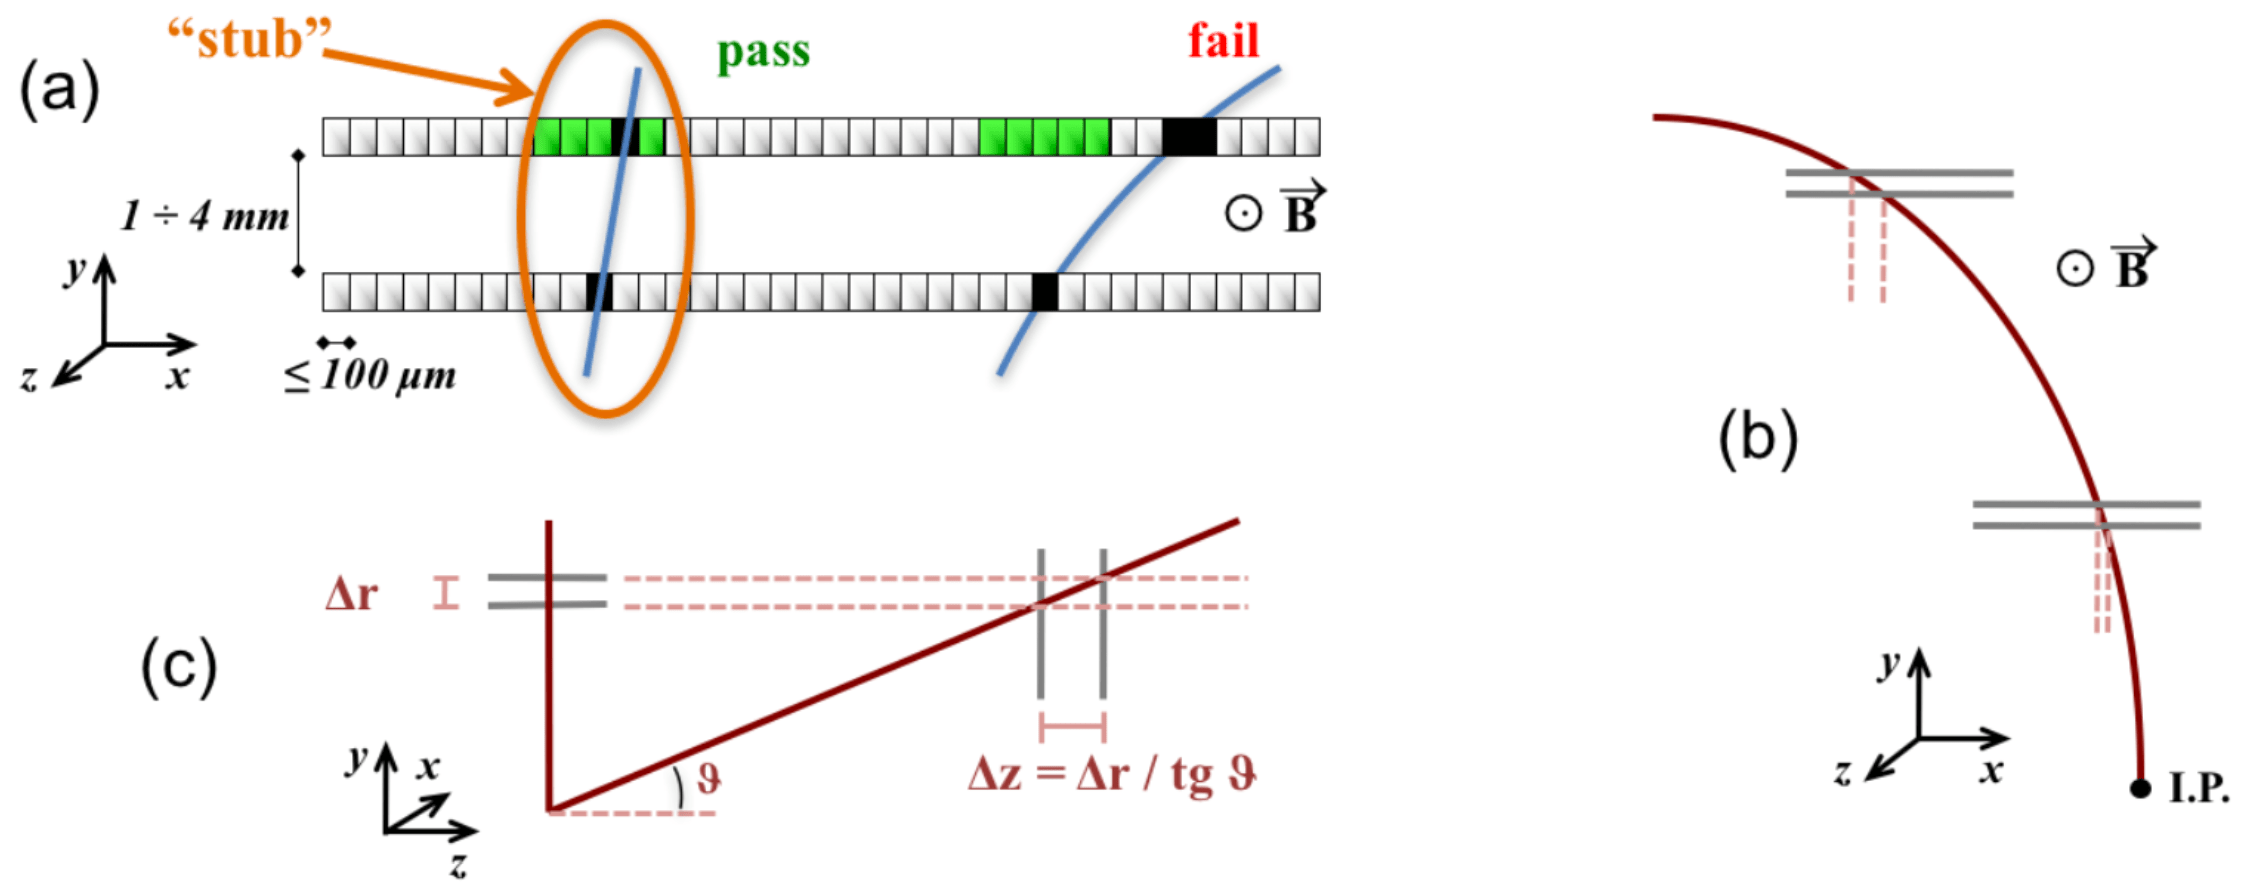
\includegraphics[width=0.99\textwidth]{Immagini/pt_module_concept.PNG}
\caption{Illustrazione schematica del concetto di $\pt$-modulo: (a) la correlazione geometrica dei segnali nel doppietto di sensori permette di identificare le coppie di hit ({\em stub}) compatibili con particelle ad alto $\pt$ grazie a una finestra di selezione configurabile; (b) a parit\`a di spaziatura tra i sensori e di $\pt$ la finestra di selezione si amplia con la distanza dal punto di interazione; (c) per gli endcap una spaziatura tra i sensori maggiore \`e necessaria per ottenere un poter discriminante analogo al barrel.}
\label{fig:PtModuleConcept}
\end{figure}
Grazie all'intensit\`a del campo magnetico di CMS, le coppie di hit ({\em stub}) che sono geometricamente compatibili con particelle al di sopra di una soglia configurabile corrispondente a $\sim 2-3\GeV$ in $\pt$ sono selezionate e inviate al sistema di trigger di L1 ogni $25\ns$. Tutti gli altri hit sono immagazzinati temporaneamente nelle pipeline in attesa dell'eventuale consenso di L1 per la lettura. Il potere risolutivo in $\pt$ del $\pt$-module dipende dalla distanza dal punto di interazione, dalla sua collocazione (barrel o endcap), come illustrato in~Fig.~\ref{fig:PtModuleConcept} e richiede un'ottimizzazione della spaziatura tra i sensori e della finestra di selezione in funzione del posizionamento. A causa della vicinanza al punto di interazione, il concetto di $\pt$-module \`e inefficace per $R\lesssim20\cm$ e per questo motivo l'IT non partecipa all'architettura del track trigger.

Il progetto di OT prevede due tipologie di moduli (vd.~Fig.~\ref{fig:TkLayoutPhaseII}): moduli 2S costituiti da due sensori $\sim10\cm\times10\cm$ con strisce lunghe $\sim5\cm$ di passo $100\um$ per la parti pi\`u esterne; moduli PS costituiti da due sensori $\sim10\cm\times5\cm$, uno a strisce di lunghezza $\sim2.5\cm$ e passo $100\um$, uno a {\em macro-pixel} di dimensione $2.5\mm\times100\um$. In entrambi i casi l'elettronica di prossimit\`a legge entrambi i sensori per poter implementare il concetto di $\pt$-module sopra descritto. Ciascun modulo ospita anche un circuito DCDC di conversione PoL per le tensioni LV e viene pilotato direttamente dal sistema di alimentazione remoto con tensioni pari a $10-12\V$. Tenendo conto anche dell'HV, l'OT richiede complessivamente $\sim90\kW$ e l'utilizzo della conversione PoL permette di minimizzare il materiale passivo associato ai cavi di alimentazione.

La potenza dissipata dal tracciatore di fase-2 \`e rimossa da un capillare sistema di raffreddamento a CO$_2$.

%\end{itemize}


%
%---------------------------------------------------------------------------------------------------------------------
%


\subsection{L'Inner Tracker, il tracciatore interno a pixel}

Il tracciatore per HL-LHC pi\`u interno o Inner Tracker (IT) merita una descrizione pi\`u approfondita essendo l'ambito in cui si \`e articolato il presente lavoro di tesi. Come visibile in~Fig.~\ref{fig:ITRzView}, l'IT \`e composto di moduli a pixel organizzati in quattro strati barrel ({\em TBPX}) per $|z|\lesssim20\cm$ e 8+8 dischi piccoli che costituiscono la parte in avanti fino a $|z|\sim160\cm$ ({\em TFPX}). TBPX e TFPX sono confinati entro $r\lesssim20cm$. Per $|z|\gtrsim160\cm$, per esigenze di integrazione e istallazione, i confine radiale tra OT e IT \`e $R\sim28\cm$. Questa regione \`e equipaggiata con una estensione costituita da 4+4 dischi grandi ({\em TEPX}). Una vista $xy$ della geometria di TBPX, TFPX e TEPX \`e visibile in~Fig.~\ref{fig:ITxyView}. 
\begin{figure}
\centering
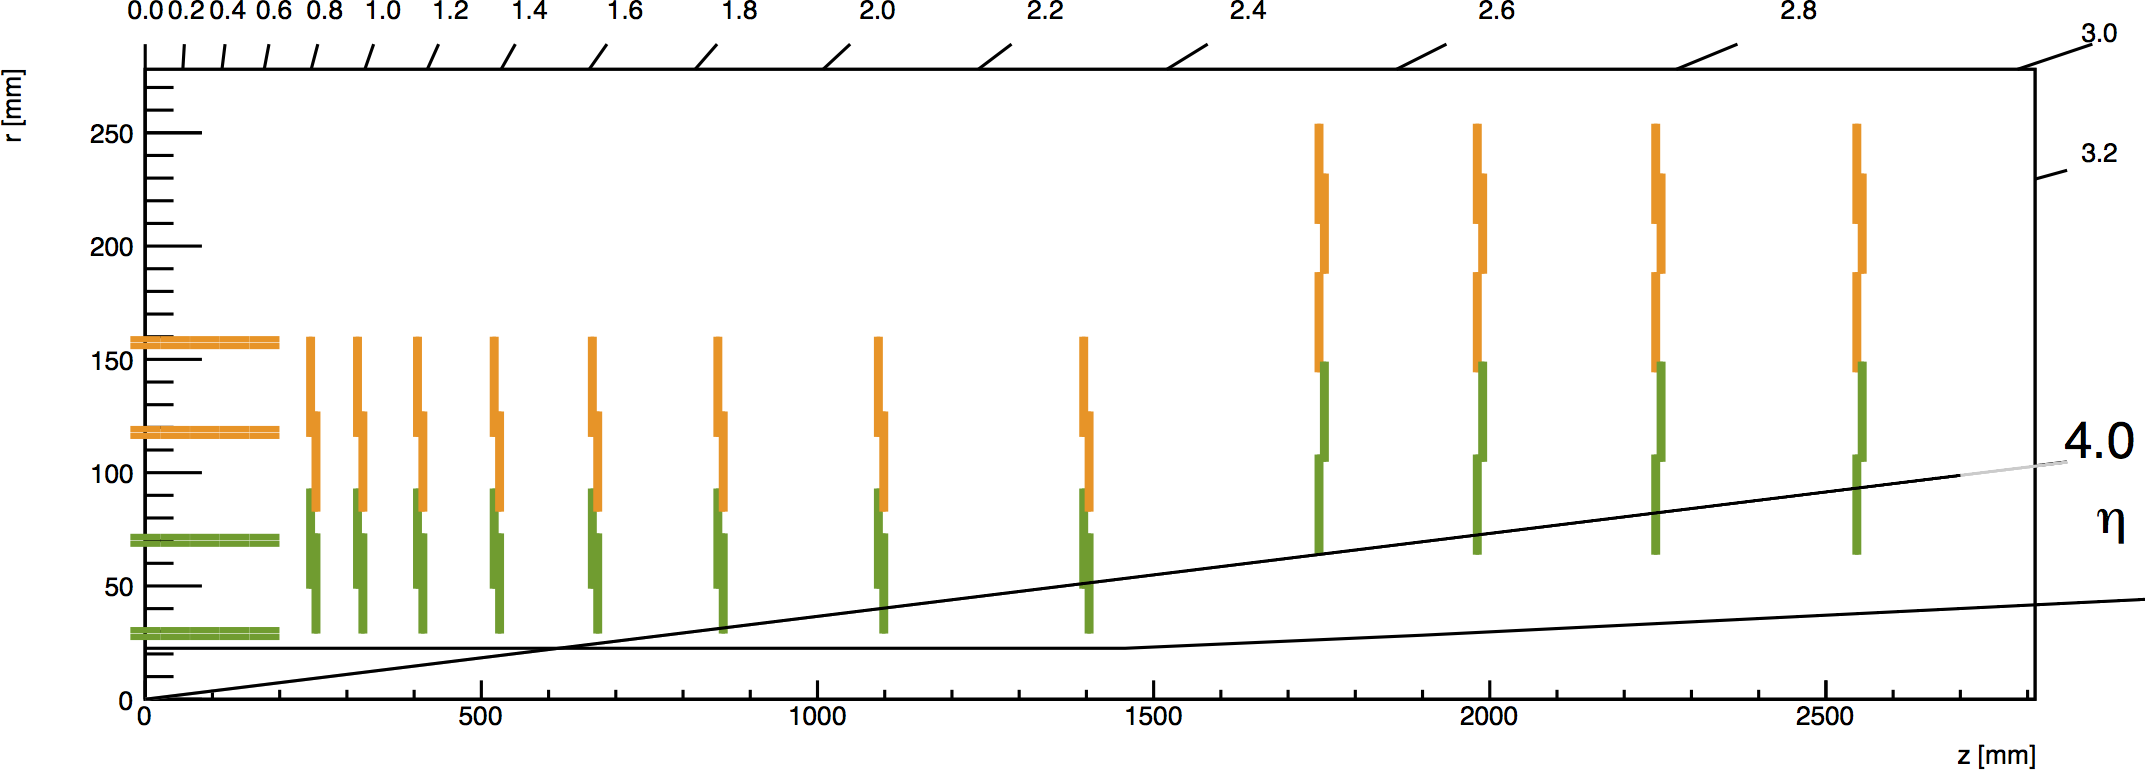
\includegraphics[width=0.99\textwidth]{Immagini/ITRzLayout.png}
\caption{Geometria di un quadrante dell'Inner Tracker nella vista $Rz$. I segmenti verdi e gialli rappresentano i moduli 1x2 e 2x2, rispettivamente. La parete della beam pipe, che ha raggio costante fino a $|z|\sim 150\cm$ \`e anch'essa visibile.}
\label{fig:ITRzView}
\end{figure}
%
\begin{figure}
\centering
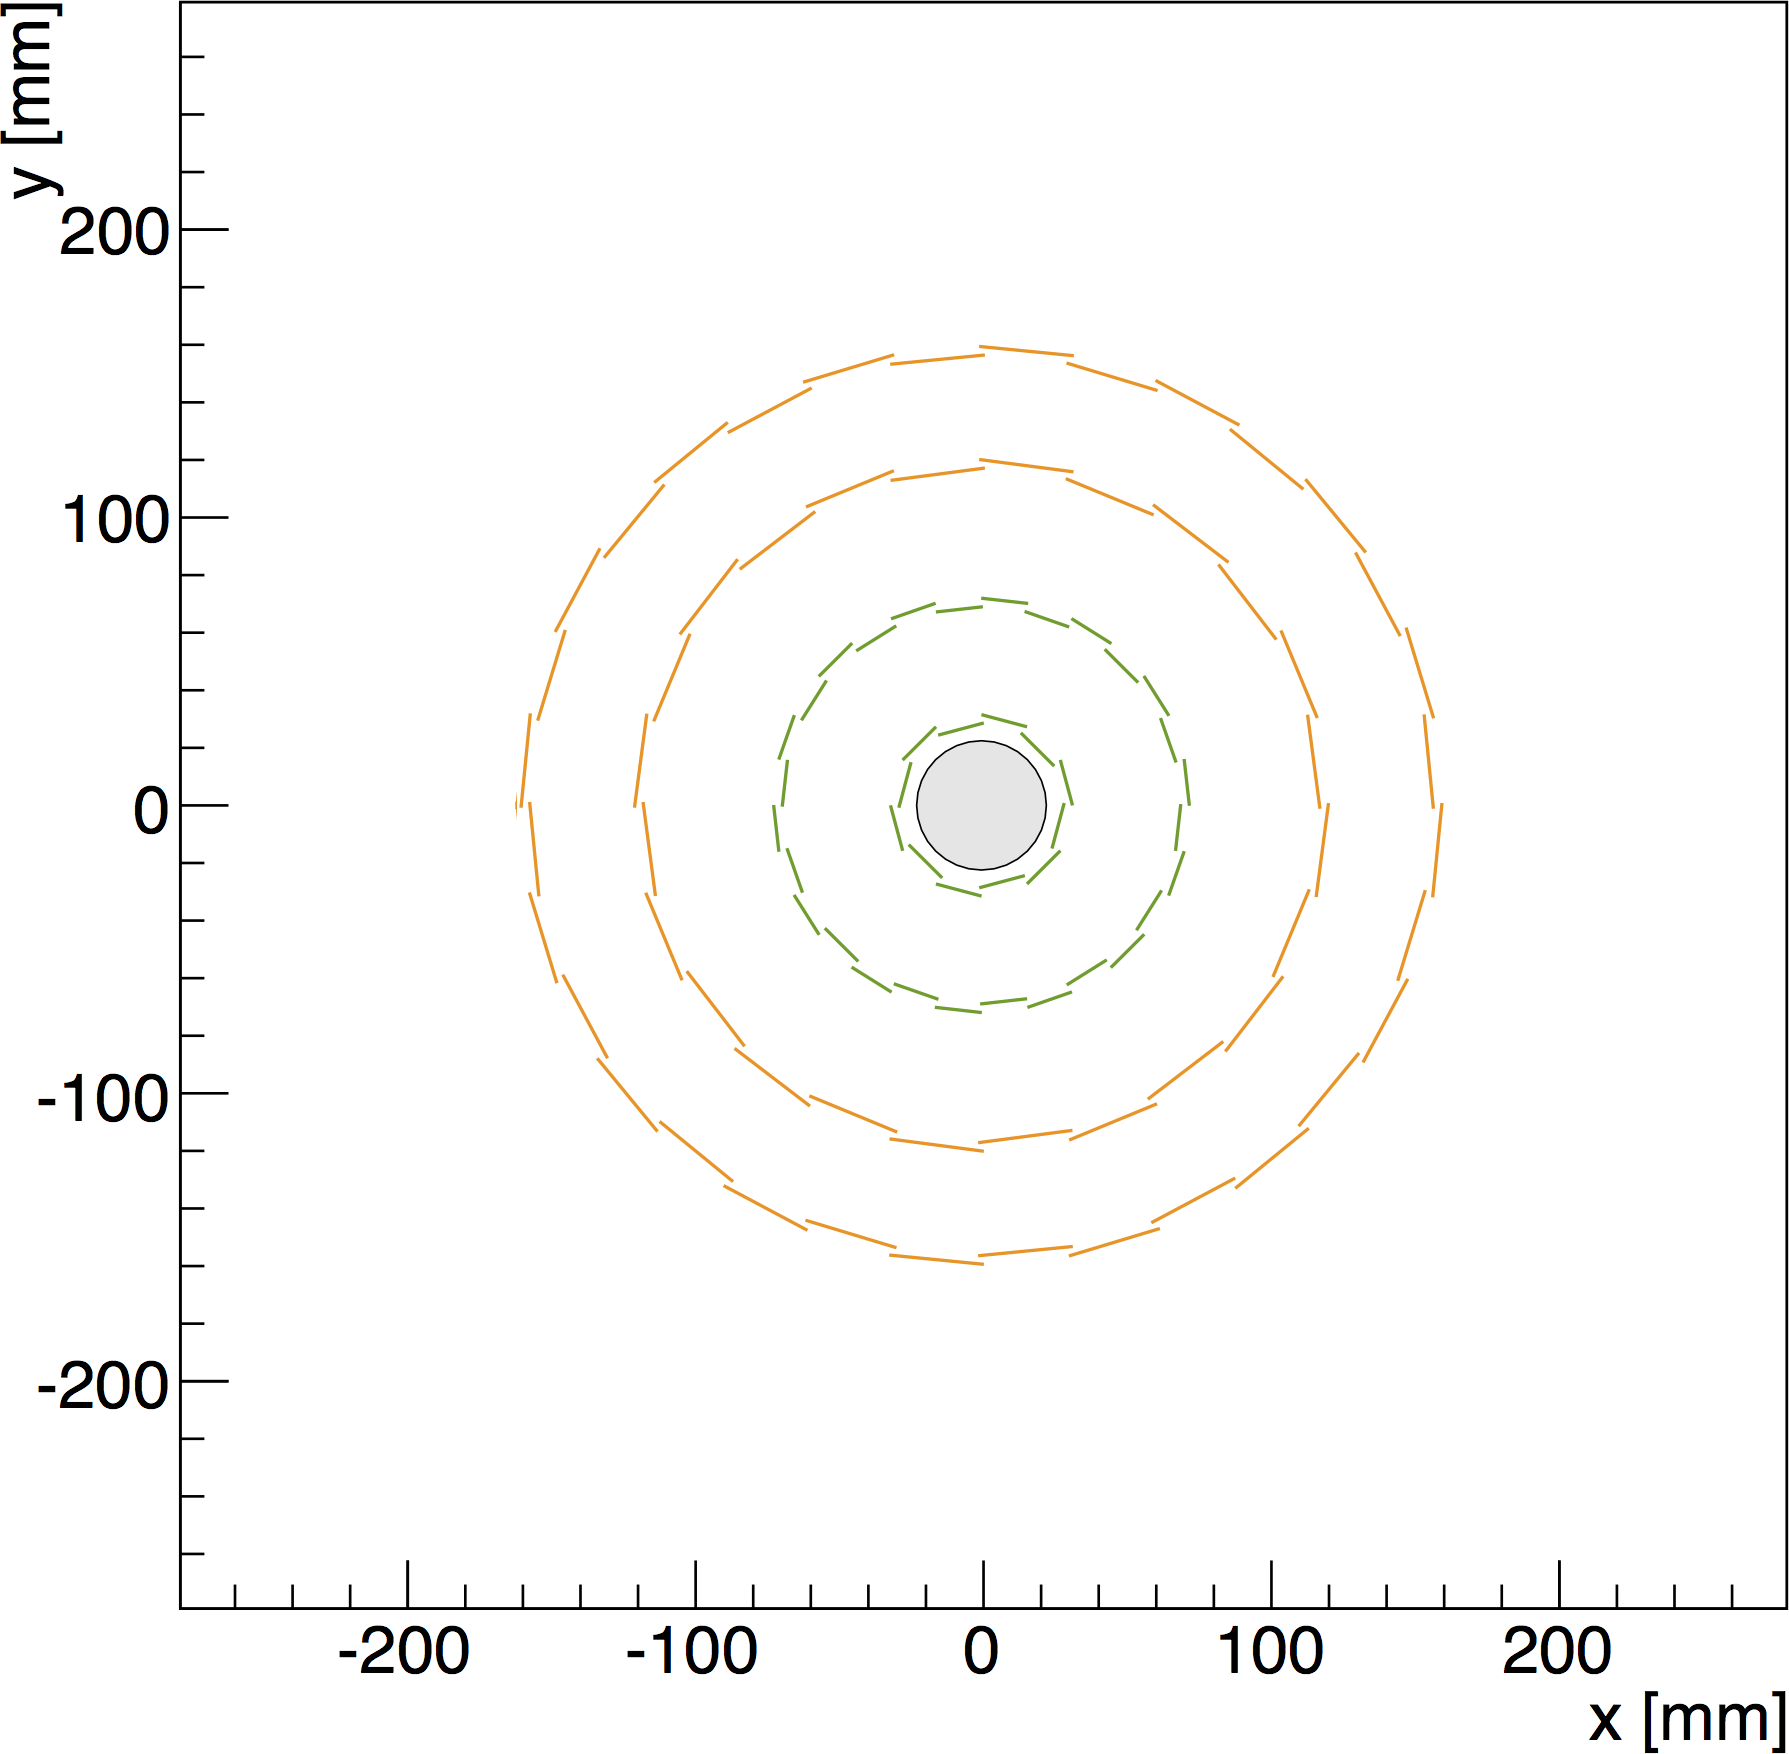
\includegraphics[width=0.3\textwidth]{Immagini/ITxyTBPX_scaled.PNG}
\hfill
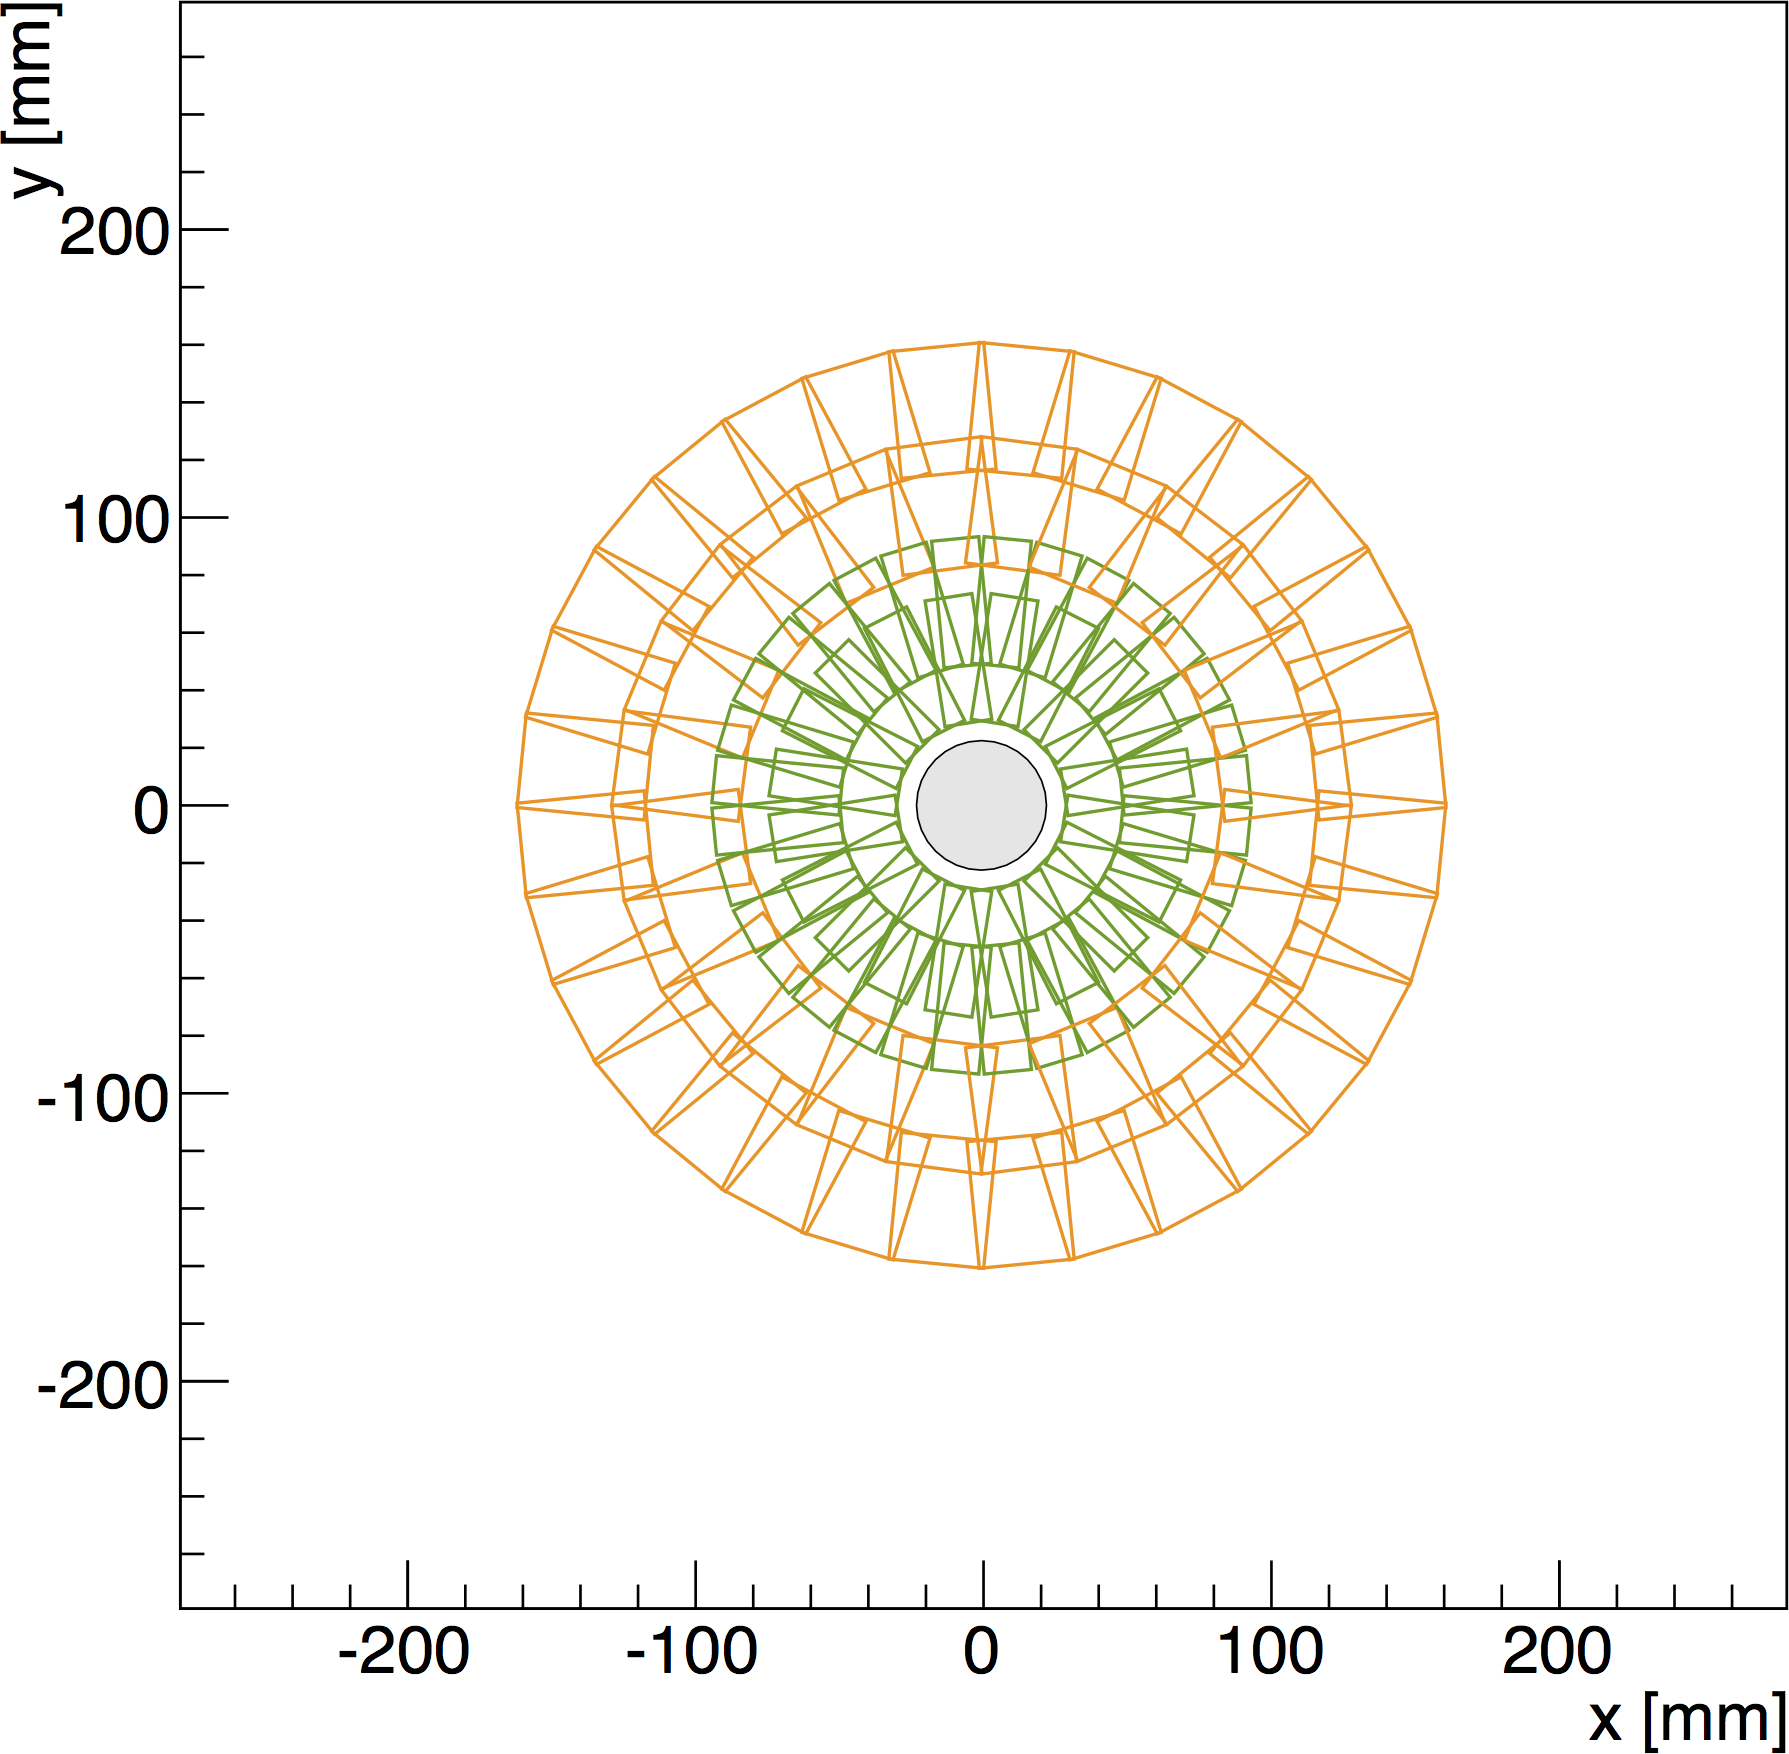
\includegraphics[width=0.3\textwidth]{Immagini/ITxyTFPX_scaled.PNG}
\hfill
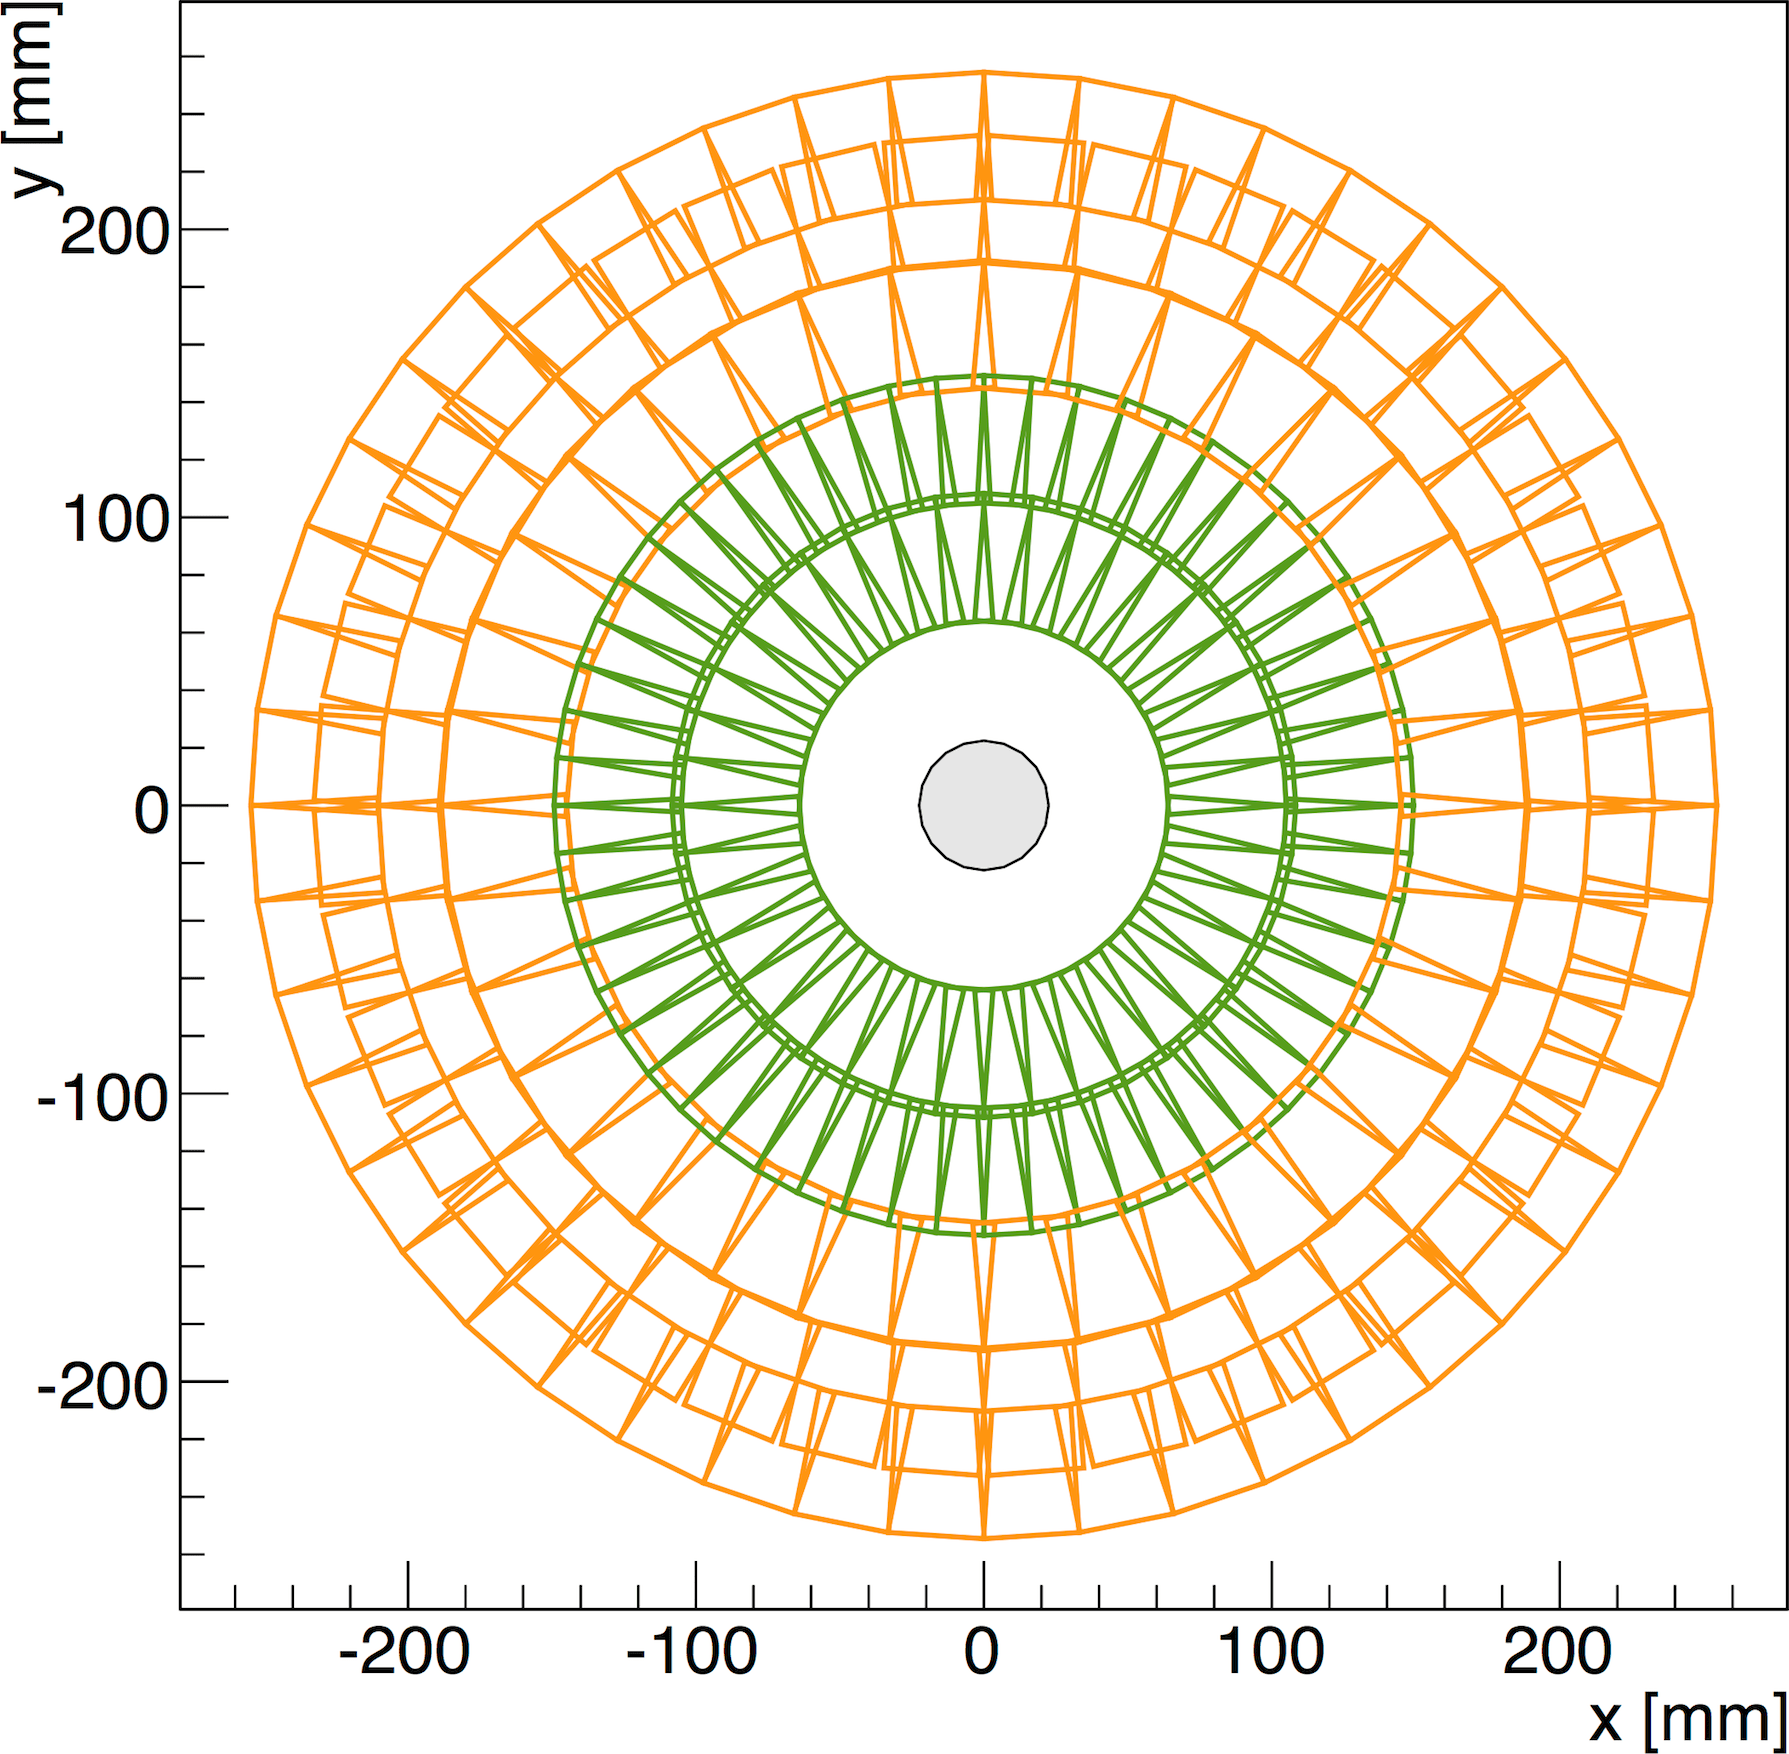
\includegraphics[width=0.3\textwidth]{Immagini/ITxyTEPX.PNG}
\caption{Vista $xy$ della geometria del TBPX, TFPX e TEPX; i segmenti o i poligoni verdi e gialli rappresentano i moduli 1x2 e 2x2, rispettivamente. L'impronta della beam pipe \`e rappresentata dal cerchio centrale.}
\label{fig:ITxyView}
\end{figure}

 I tre sottosistemi sono visibili in prospettiva in~Fig.~\ref{fig:ITPerspectiveView} insieme alla superficie di supporto detta anche {\em service cylinder} perch\`e su di essa sono organizzati i servizi necessari all'apparato (cavi di alimentazione, connessioni di readout, tubi di raffreddamento). 
\begin{figure}
\centering
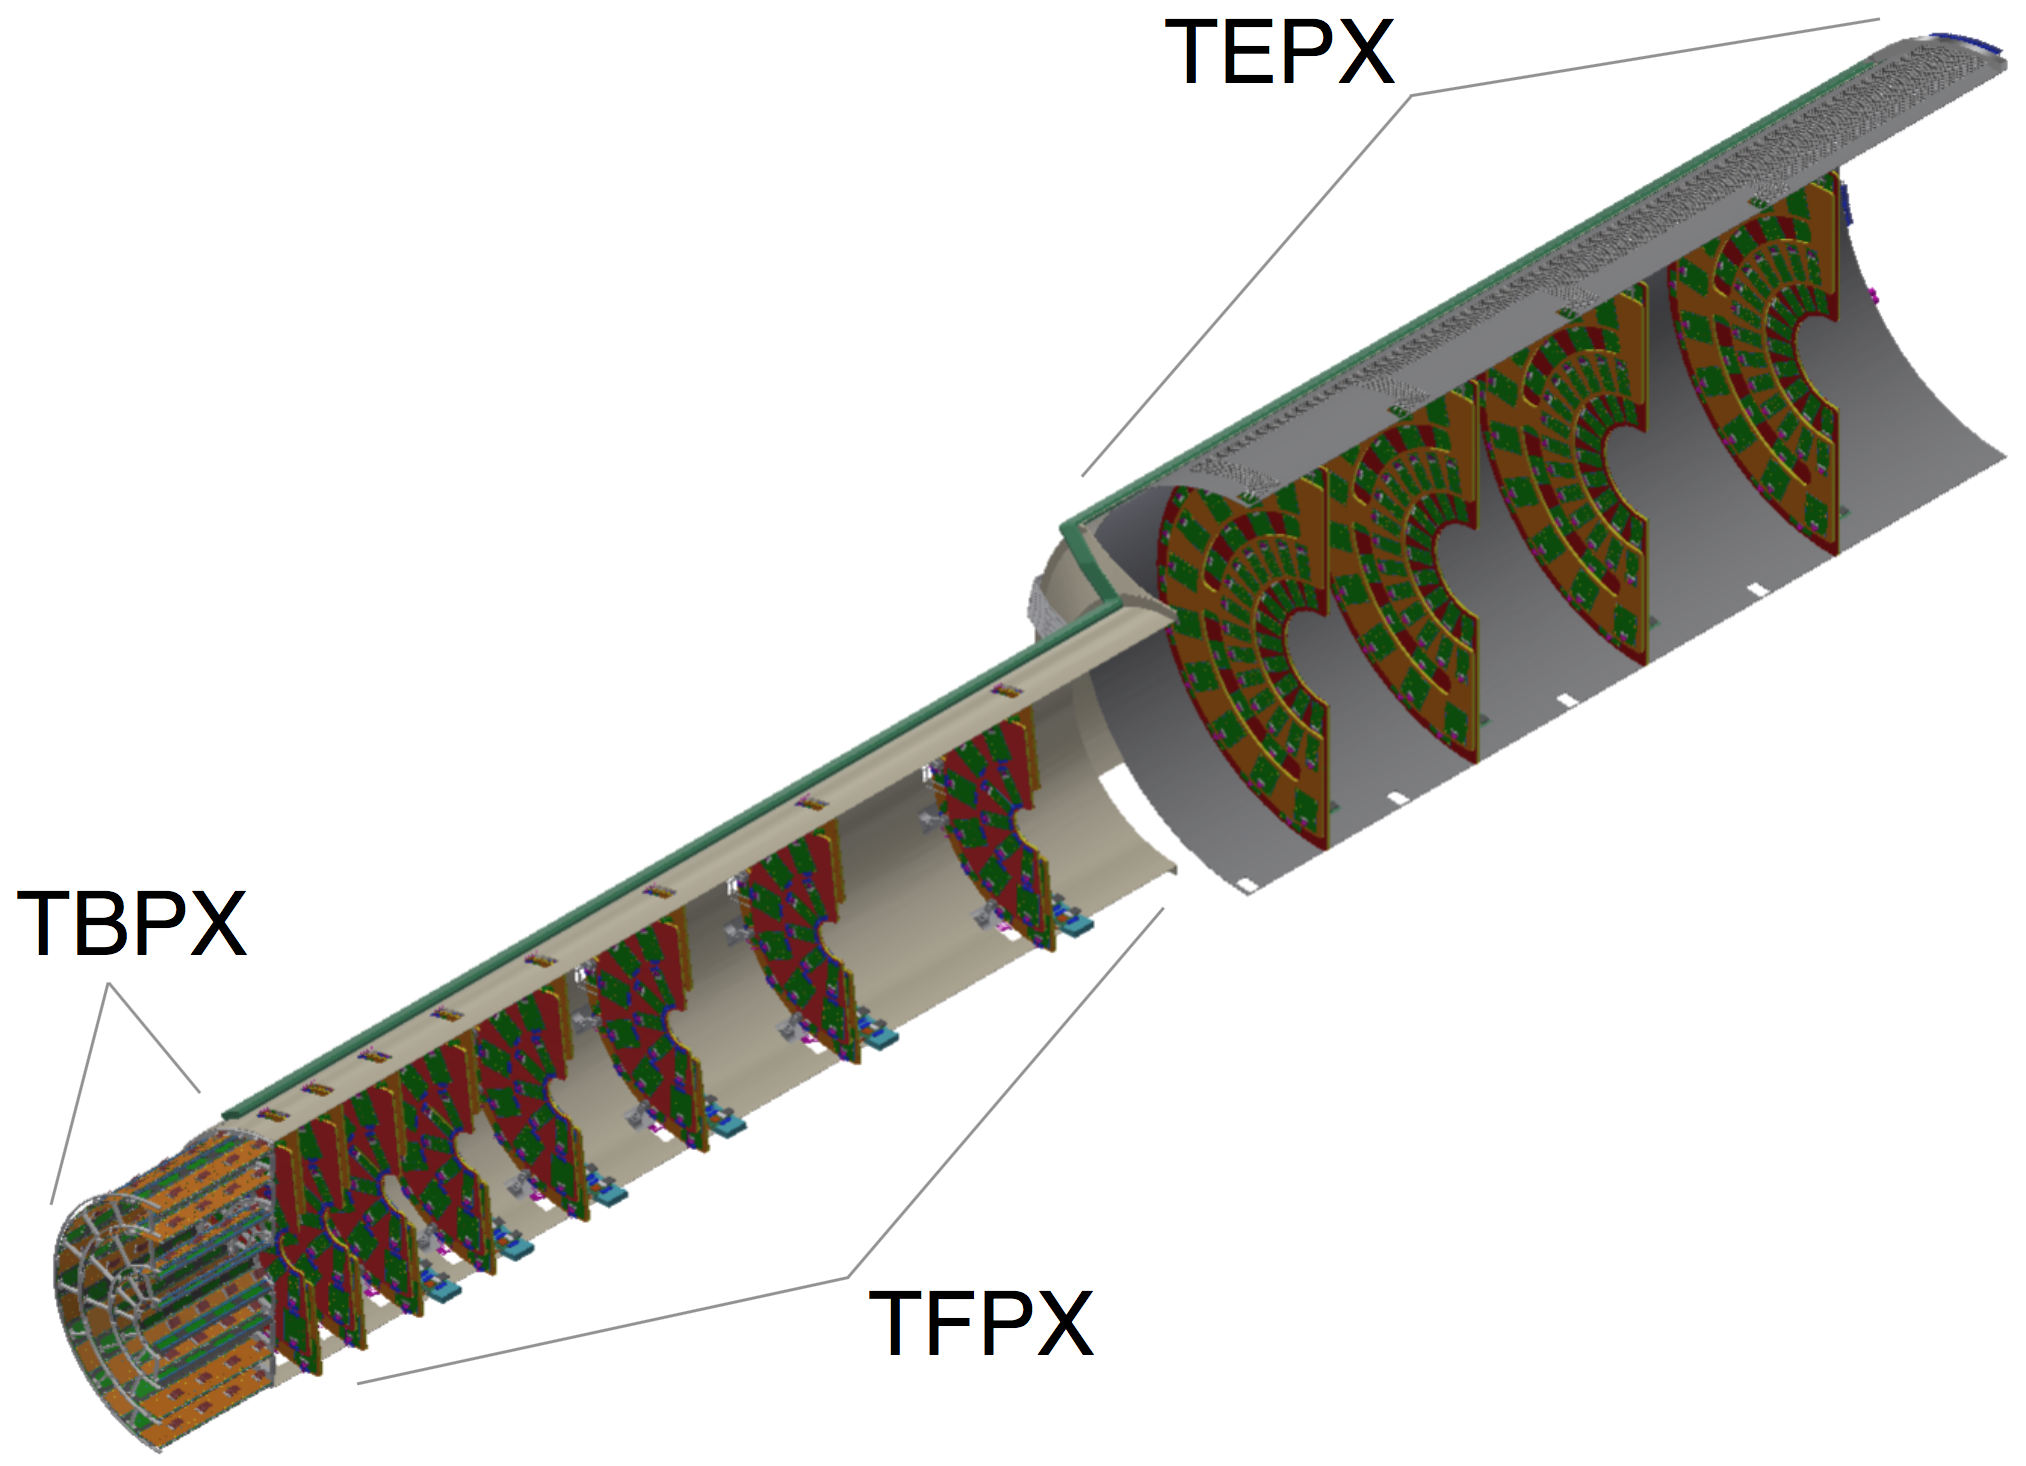
\includegraphics[width=0.99\textwidth]{Immagini/ITPerspectiveView.PNG}
\caption{Vista prospettica di un quarto dell'IT, in cui sono mostrati i tre sottosistemi all'interno del service cylinder.}
\label{fig:ITPerspectiveView}
\end{figure}


L'IT sar\`a il sottosistema maggiormente sottoposto alla radiazione indotta dall'aumento di luminosit\`a di HL-LHC, come illustrato in~Fig.~\ref{fig:fluencemap}. Il valori massimi di fluenza e di dose ionizzante per $3000\ifb$, pari a $2.3 \times 10^{16} \mathrm{n_{eq}\cm^2}$ e $12\MGy$ ($1.2 Grad$), sono attesi per lo strato barrel pi\`u interno ($R\sim28\mm$). Nella regione IT la radiazione in fluenza e dose \`e di fatto esclusiva funzione della distanza radiale dall'asse dei fasci. 
\begin{figure}
\centering
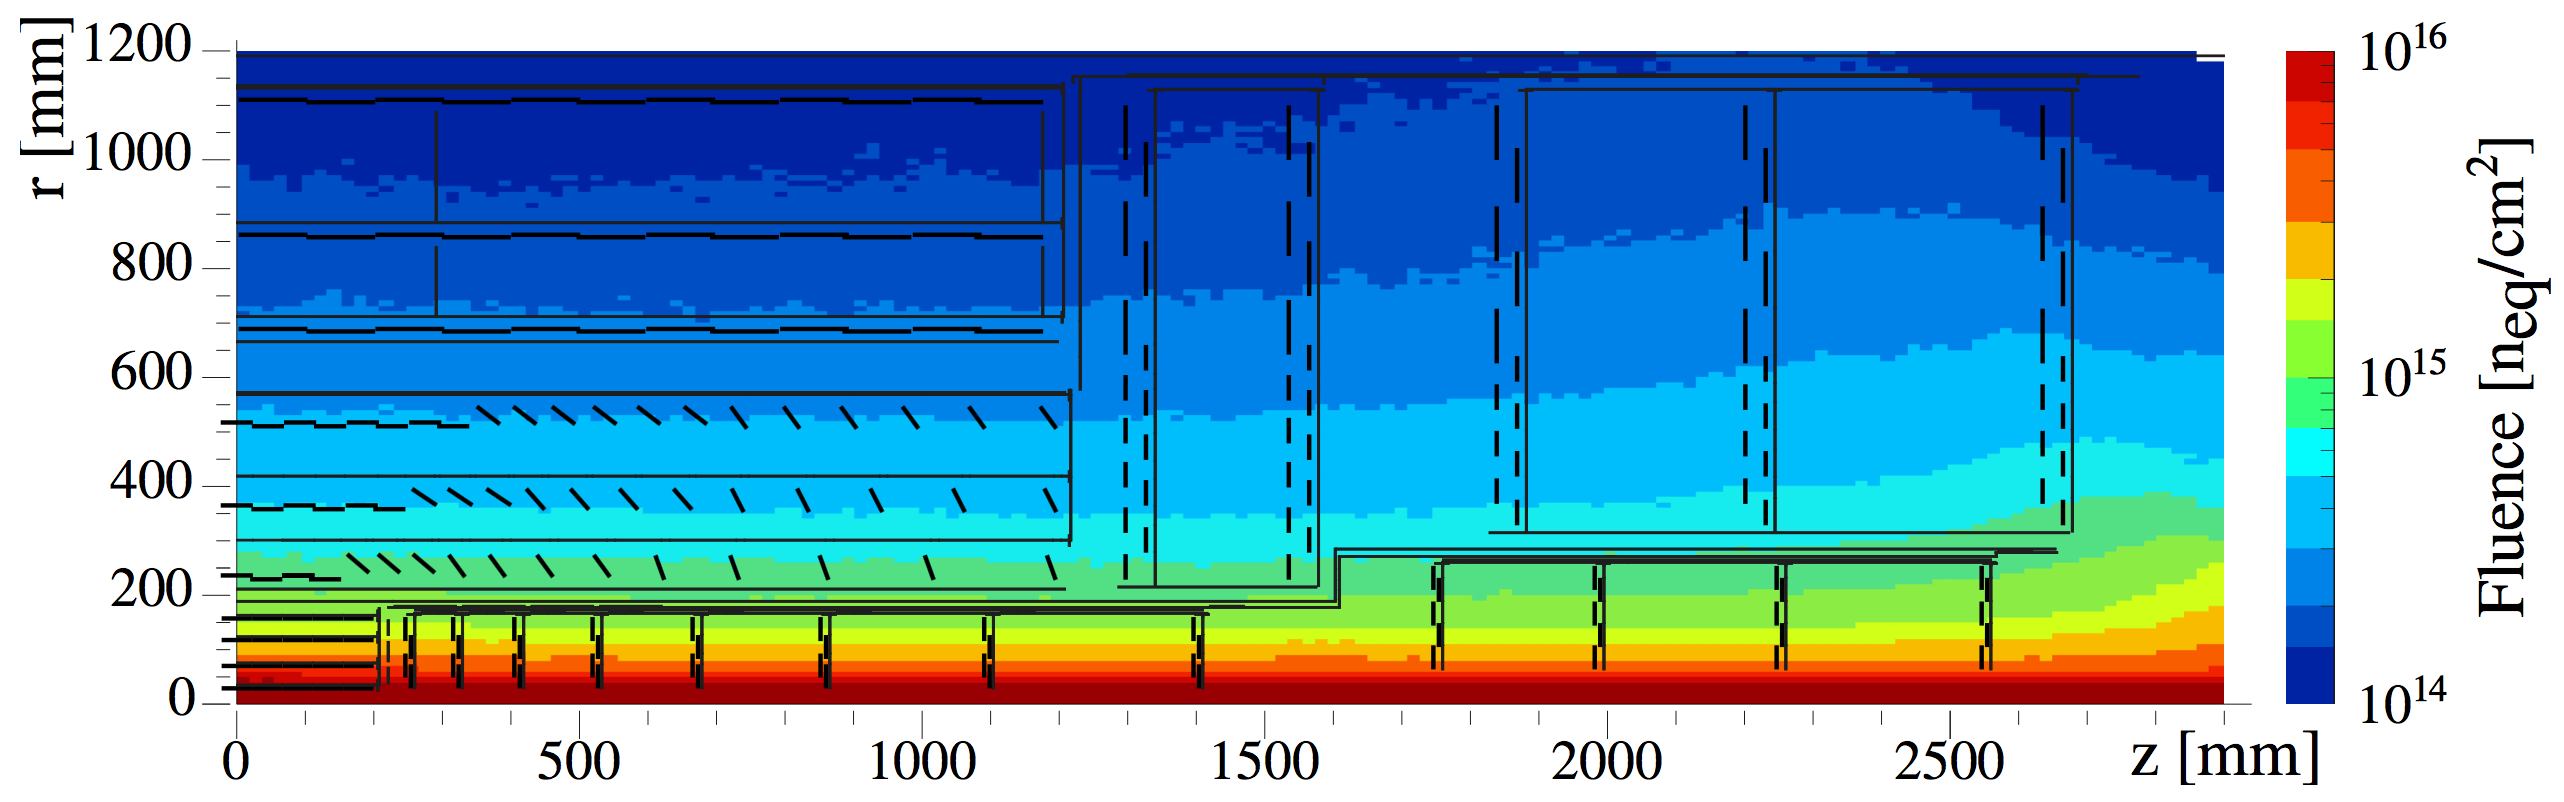
\includegraphics[width=0.99\textwidth]{Immagini/HLLHC_Fluence.PNG}
\caption{Mappa della fluenza integrata, espressa in neutroni da $1\MeV$ equivalenti a $\cm^2$, corrispondente a $3000\ifb$.}  
\label{fig:fluencemap}
\end{figure}

% \[
% \begin{array}{lccc}
% \toprule
% \mathrm{Regione} & \mathrm{Fluenza \quad massima} [n_{eq}/cm^2] & r [mm] & z[mm]  \\
% \midrule
% \mathrm{IT \quad barrel \quad layer 1} & 2.3\times10^{16} & 28 & 0\\
% \mathrm{IT\quad barrel\quad layer 2} & 5.0\times10^{15} & 69 & 0\\
% \mathrm{IT\quad barrel\quad layer 4} & 1.5\times10^{15} & 156 & 89\\
% \mathrm{IT\quad forward,\quad ring 1} & 1.0\times10^{16} & 51 & 252\\
% \mathrm{IT\quad service\quad cylinder} & 9.6\times10^{14} & 170 & 260\\
% \bottomrule
% \end{array}
% \]

Il modulo a pixel, l'elemento base dell'IT, \`e costituito da un sensore a pixel accoppiato ai relativi circuiti integrati di readout (ROC) tramite {\em bumb bonding}\footnote{Il {\em bump bonding} \`e una tecnologia che utilizza sferette (di $10-50\um$ di diametro) di opportuna lega saldante per connettere le piazzole di due circuiterie integrate affacciate l'una contro l'altra.}. Il modulo \`e completato da un circuito stampato su supporto flessibile (detto {\em high density interconnect}, HDI) che ospita il resto della componenstistica ancillare (connettori, componenti passivi e eventuali altri ASIC) connesso ai ROC tramite microsaldature e dal supporto meccanico.

%
% ---------------------------------------------------------------------------------------------
%
 
L'IT si base su sensori con pixel di dimensione $25\times100\um^2$ o $50\times50\um^2$ (un fattore $6\times$ inferiore all'attuale pixel di fase-0). Due opzioni tecnologiche sono prese in considerazione per soddisfare al requisito di resistenza alla radiazione: una pi\`u tradizionale tecnologia planare in cui i pixel sono realizzati con impianti n-su-p e la tecnologia cosiddetta {\em 3D}, pi\`u innovativa, in cui la segmentazione in celle del sensore avviene tramite la realizzazione di impianti a colonna che attraversano lo spessore del cristallo.

Nel caso planare la resistenza alla radiazione si basa sull spessore sottile del volume attivo, compreso tra $100$ e $150\um$. Il danneggiamento da radiazione induce la creazione di difetti di trappola nel silicio che limitano il percorso delle cariche generate da particella. La minimizzazione di questo percorso rende l'efficienza di collezione di carica meno dipendente dall'irraggiamento. La riduzione dello spessore attivo richiede per\`o un'elettronica di lettura pi\`u raffinata compatibile con un segnale tipico di particella pi\`u piccolo.

Nel caso dei sensori 3D il cammino di raccolta delle cariche di segnale \`e ulteriormente ridotto dal momento che gli elettrodi di giunzione sono verticali e la loro distanza tipica \`e determinata dalle dimensioni della cella e non dallo spessore attivo del sensore. I sensori 3D, intrinsecamente pi\`u resistenti alla radiazione, potrebbero essere usati per equipaggiare lo strato pi\'u interno della parte barrel e i moduli destinati alle posizioni a pi\`u piccolo raggio di TFPX.

Per la diversa disposizione degli elettrodi di giunzione, un sensore pixel planare necessita di una tensione di polarizzazione pi\`u elevata di un sensore 3D. In particolare, a parit\`a di irraggiamento, che influisce molto sulla tensione necessaria per un completo svuotamento del sensore, si parla di qualche centinaio di V per i planari contro qualche decina di V per i 3D.

%
% ---------------------------------------------------------------------------------------------
%

Il ROC che \`e in fase di sviluppo per l'IT \`e avr\`a un'area attiva, cio\`e corrispondente alla matrice dei pixel, di $16.4\times22.0\mm^2$, pari a $328\times440$ celle di $50\times50\um^2$. Con un'opportuna disposizione delle piazzole per il bump bonding questo ROC pu\`o leggere anche sensori con pixel di $25\times100\um^2$. I moduli sono previsti essere di soli due soli tipi di moduli, differenziati esclusivamente dall'area attiva del sensore e dal numero di ROC. Il modulo {\em 1x2}, di $\sim16.4\times44\mm^2$ di area attiva, equipaggia le regioni a pi\`u piccolo raggio come mostrato nelle Figure~\ref{fig:ITRzView,fig:ITxyView} dove \`e pure visibile il mosaico dell'altra tipologia di moduli, {\em 2x2}, di $\sim32.8\times44\mm^2$ di area attiva, concepiti per le regioni pi\`u distanti dall'asse dei fasci.

Il disegno dei moduli come risulta dal progetto che viene sviluppato attualmente \`e visibile in~Fig.~\ref{fig:ITModSkecth}.
\begin{figure}
\centering
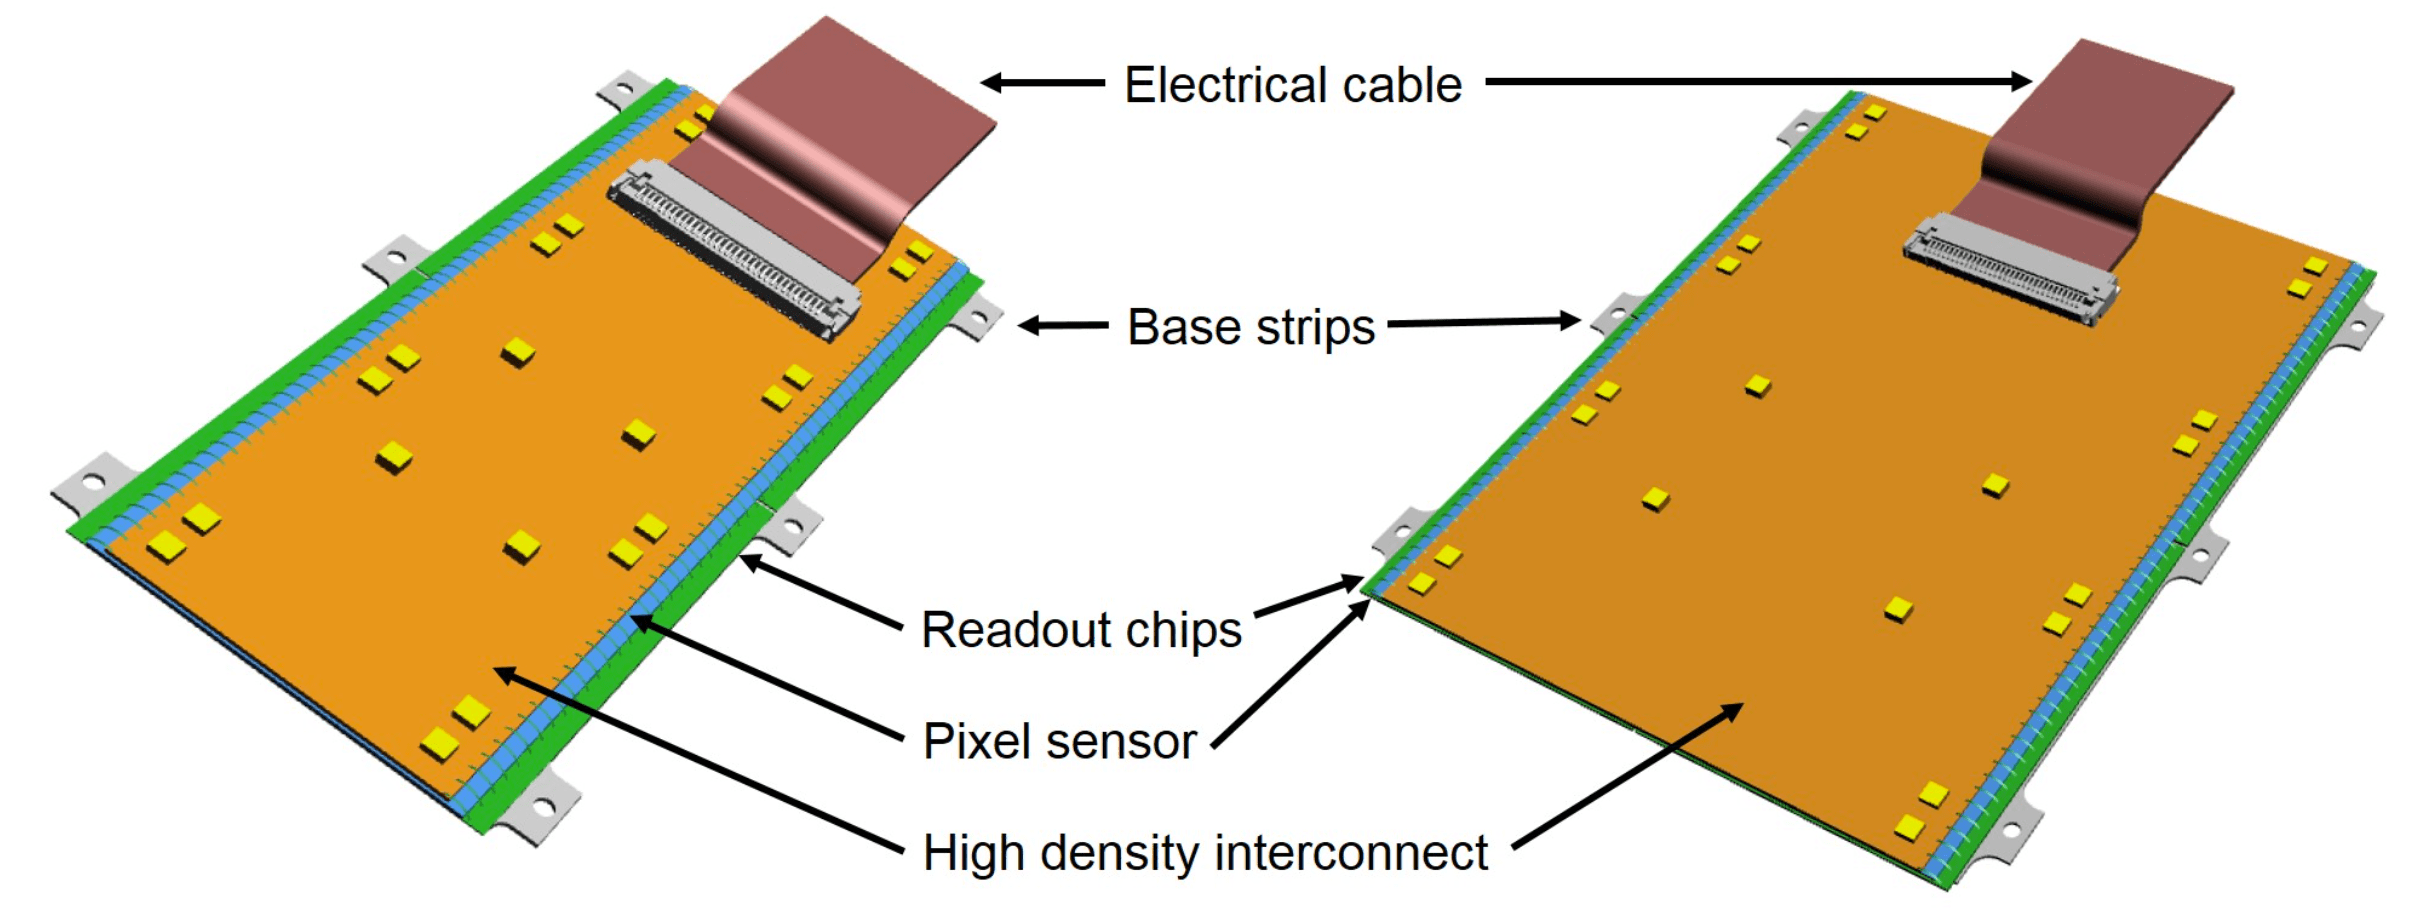
\includegraphics[width=0.8\textwidth]{Immagini/ITModSkecth.PNG}
\caption{Disegno CAD dei moduli IT 1x2 (sinistra) and 2x2 (destra). Tenendo conto della `periferia' del ROC (dove sono collocate le piazzole per le microsaldatura) le dimensioni fisiche sono  $\sim1.8\times4.4\cm^2$ e  $\sim3.7\times4.4\cm^2$, rispettivamente.}  
\label{fig:ITModSkecth}
\end{figure}


% \subsubsection{Sensori}
% \begin{figure}
% \centering
% 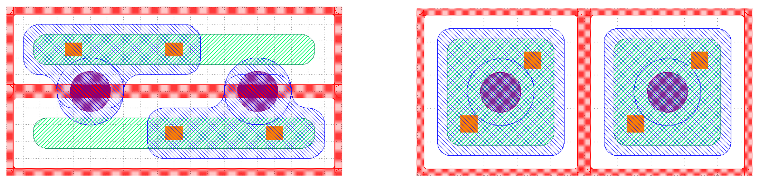
\includegraphics[scale=0.35]{Immagini/Sensors}
% \caption{Schema di due celle adiacenti con dimensioni $\mathrm{25 \times 100 \mu m^2}$ (sinistra) e $\mathrm{50 \times 50\mu m^2}$ (destra). Gli impianti n+ sono riportati in verde, in blu le metallizzazioni, in rosso le aree di p-stop , i contatti in arancione e in viola i le piazzole per i bump bond.}
% \label{Sensors}
% \end{figure}

\subsubsection{Il ROC per l'IT}

Il ROC, il componente pi\`u critico per l'Inner Tracker, deve essere resistente alla radiazione, a bassa soglia e basso rumore, adatto quindi ai segnali di rivelatori sottili, a grande banda di lettura e, infine, le celle di $2500 \um^2$ richiedono una miniaturizzazione spinta. La collaborazione RD53 (referenza rd53), un progetto comune di Atlas e CMS per lo sviluppo di pixel ROC per HL-LHC,  st\`a sviluppando questo ROC nella tecnologia CMOS a $65\nm$ che, sulla carta, \`e  compatibile con i succitati requisiti.

Il diagramma a blocchi del progetto concepito da RD53 è mostrato in Fig.~\ref{ChipBlockDiagram}. 
\begin{figure}
\centering
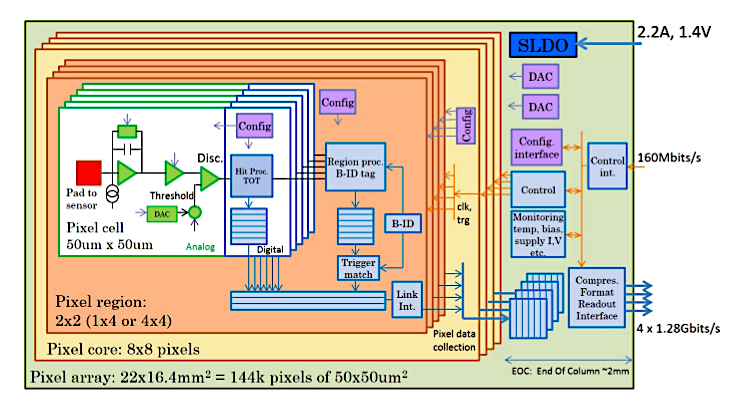
\includegraphics[scale=0.4]{Immagini/ChipBlockDiagram}
\caption{Architettura del chip con bassi livelli di rumore analogico con un sistema di digitalizzazione del ToT a 4 bit. Nello schema sono riportate anche l'interfaccia di controllo, posta nella zona di EOC (End Of Column), l'interfaccia di lettura e il sistema di alimentazione che sfrutta un regolatore di tensione con shunt (Shunt-LDO).}
\label{ChipBlockDiagram}
\end{figure}
Ciascun pixel \`e connesso in DC al relativo canale di lettura del chip tramite bump bonding. La carica cos\`i raccolta entra nello stadio di preamplificazioe/formazione per essere infine digitalizzata con una risoluzione di 4 bit a 40 MHz sfruttando il metodo del {\em Time Over Threshold} (TOT). Questo consiste nello stimare l'entit\`a del segnale, correlato alla carica raccolta, misurando, in colpi di clock, il tempo durante il quale l'impulso a valle degli stadi di preamplificazione è al sopra di una certa soglia. I segnali digitalizzati, organizzati in gruppi di 2x2 pixel adiacenti detti {\em pixel region}, vengono quindi immagazzinati localmente in vettori di memoria per non pi\`u di $12.5\us$ in attesa dell'eventuale consenso del trigger di Livello 1. In presenza di quest'ultimo i dati relativi al bunch crossing corrispondente sono estratti dalla memoria e, opportunamente compressi, sono indirizzati su linee differenziali digitali elettriche ({\em e-link}) da 1.28Gb/s ciascuna, ma configurabili in numero (da 1 a 4) per garantire una banda passante sufficiente anche nelle regioni pi\`u interne. I ROC possono essere concatenati per condividere gli e-link in modo da ottimizzarne il numero per i moduli che equipaggiano le regioni pi\`u esterne e che quindi richiedono un banda passante limitata. La distanza da percorrere per raggiungere il sistema di DAQ, pari a qualche decina di metri, non \`e per\`o compatibile con un protocollo di trasmissione elettrico. Opportuni opto-convertitori basati sul chipset LpGBT (ref ) e su VL+ (ref ) per il pilotaggio del laser, convogliano i dati di 7 e-link in una linea ottica in fibra da 10Gb/s. Questi convertitori sono ospitati sul service cylinder data la loro limitata resistenza alla radiazione che impone che non siano collocati a meno di $R\sim20\cm$ dall'asse dei fasci. Tale posizionamento \`e per\`o compatibile con gli e-link che hanno una portata di ${\cal O}(\m)$ senza che i segnali digitali siano irrimediabilmente degradati.
Tramite una linea ottica a 2.5Gb/s, il convertitore LpGBT riceve anche i segnali relativi al clock, al trigger, ai comandi e ai dati di configurazione necessari per il funzionamento dei ROC che sono poi convogliati in e-link dedicati a 160Mb/s. 

Il ROC implementa una circuiteria di calibrazione tramite la quale \`e possibile iniettare in tutti i canali un impulso configurabile in ampiezza e temporizzazione. \`E inoltre presente una estesa rete di controllo del funzionamento del ROC grazie a sensori di temperatura e al monitoraggio delle alimentazioni, dei valori di tensione e di correnti di polarizzazione della parte analogica del dispositivo.

%
% --------------------------------------------------
%

%All power supply voltages (before and
%after the power regulator) and currents can be measured. In addition, a large number of ana-
%logue operation parameters can be monitored: bias currents for analogue front-ends, band gap
%references, calibration pulse voltages, PLL control voltage, etc. Dedicated features to monitor
%radiation degradation at both single transistor level and digital level (ring oscillators) are also
%included.
Un rapido elenco delle caratteristiche del chip di lettura sono riportate in tabella:

\[
\begin{array}{ll}

\toprule

\midrule

\mathrm{Technology} & \quad 65 \mathrm{nm \quad CMOS}\\

\mathrm{Chip \quad size} & \quad \mathrm{22 mm \times (16.4 mm + 2 mm)} \\

\mathrm{Pixel \quad size} & \quad \mathrm{50 \times 50 \mu m^2, 25 \times 100 \mu m^2)} \\

\mathrm{Number\quad of\quad pixels} & \quad \mathrm{144320} \\

\mathrm{Hit \quad rate} & \quad \mathrm{< 3 GHz/cm^2} \\

\mathrm{Charge \quad resolution} & \quad \mathrm{24 bit \quad ToT} \\


\bottomrule
\end{array}
\]

%si può allungare la lista

Pur utilizzando la tecnologia CMOS ad alta densit\`a (65nm) caratterizzata da limitata tensione di alimentazione ($\sim 1.2\V$) e consumi ridotti si stima che il ROC di CMS abbisogni di $\sim 2.2\A$ per il suo funzionamento, pari a $\sim 0.5\W/\cm^2$, equamente suddivisi tra parte analogica (i circuiti di preamplificazione) e digitale (readout e controlli). La prima richiede elevate correnti perch\'e, a causa della necessit\`a di avere soglie basse, la corrente di polarizzazione del primo stadio di amplificazione deve essere elevata per contenere il rumore. I consumi della parte digitale sono invece dovuti all'elevato rate di lettura. In situazioni limite la richiesa di potenza pu\`o ulteriormente aumentare.

Nel suo complesso, dati i 1960 moduli 1x2 e i 2392 moduli 2x2, l'intero IT richiede $\sim13500$ ROC per un consumo totale per la sola elettronica di prossimit\`a pari a $\sim 35\kW$. Per quanto precedentemente esposto tale potenza non pu\`o essere fornita con uno schema di alimentazione diretta perch\'e questo richiederebbe cavi di grande sezione per contenere le perdite e quindi un ammontare di materiale passivo tale da inficiare pesantemente le prestazioni dell'IT. Sono state valutati, quindi, schemi di alimentazione a tensione intermedia con conversione `PoL'.

Il possibile approccio, analogo all'attuale rivelatore a pixel di fase-1, consiste nell'utilizzo di convertitori DCDC. Questi per\`o sono afflitti da due importanti limitazioni che rendono questo approccio non percorribile. La prima: essendo dispositivi di potenza, la resistenza alla radiazione degli ASIC su cui si basano i convertitori DCDC \`e limitata e questi non potrebbero essere piazzati a meno di $R\sim20-25\cm$ dall'asse dei fasci con la conseguenza che gli ultimi ${\cal O}(10-100\cm)$ di trasmissione di potenza dovrebbe comunque avvenire a tensione di utilizzo, vicino al V, richiedendo cavi di opportuna sezione vanificando cos\`i la riduzione di materiale nella regione pi\`u critica. La seconda: i convertitori DC/DC richiedono induttanze di dimensioni generose che, a causa del campo magnetico a grande intensit\`a in cui sarebbero immerse, devono necessariamente essere avvolte su nuclei ferromagnetici. I convertitori DC/DC risultano quindi oggetti a scarsa miniaturizzazione e piuttosto pesanti essi stessi da rendere impossibile (per ragioni di spazio) e controproducente (a causa del materiale passivo) la loro collocazione sul cilindro dei servizi gi\`a affollato dalla presenza dei moduli LpGBT e degli altri servizi. A causa della minore densit\`a di canali e della pi\`u grande distanza dall'asse dei fasci queste limitazioni sono compatibili con l'utilizzo dei convertitori DCDC nell'OT.

L'unico approccio che \`e stato valutato compatibile con i requisiti dell'IT \`e uno schema di alimentazione seriale. Questo rappresenta una sfida senza precedenti perch\'e non \`e mai stato utilizzato su larga scala in un rivelatore per la fisica di alte energie progettato operare in condizioni limite.

L'IT \`e dunque organizzato in catene di alimentazione seriale, ciascuna composta da 8-10 moduli, con i ROC di ciascun modulo alimentati in parallelo, come rappresentato schematicamente in Fig.~\ref{serial}. 
\begin{figure}
\centering
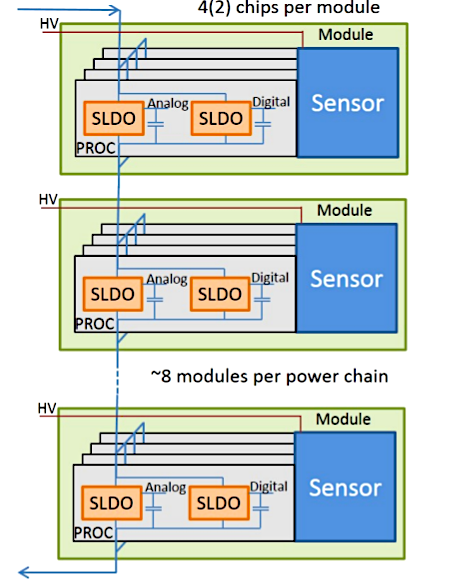
\includegraphics[scale=0.4]{Immagini/serial}
\caption{Sistema di alimentazione seriale dei moduli, ognuno dei quali ha al suo interno 4 o 2 chip in parallelo. Sul chip l'alimentazione è gestita da due SLDO in parallelo, uno per la parte digitale e uno per quella analogica.}
\label{serial}
\end{figure}
Il cuore dello schema di alimentazione seriale, che \`e approfondito nel prossimo capitolo, \`e la circuiteria ancillare integrata nel ROC stesso, detta SLDO, che implementa l'ultimo stadio di regolazione fine delle tensioni LV e assicura un consumo di corrente costante, indipendentemente dal rate di eventi e di trigger.

Riassumendo, i vantaggi di una alimentazione seriale sono i seguenti:
\begin{itemize}
\item la conversione tra la tensione intermedia di alimentazione della catena e la tensione prossima a quella di lavoro del ROC \`e intrinseca nello schema seriale stesso per cui non sono necessari dispositivi di potenza, ovvero in grado di gestire grandi correnti a tensioni intermedie dell'ordine della decina di $\V$ compunque proibitive per tecnologie VLSI, n\'e componentistica passiva ingombrante (come, ad esempio, gli induttori necessari sui convertitori DCDC);
\item per quanto sopra, la circuiteria necessaria per l'implementazione dell'alimentazione seriale \`e compatibile con la tecnologia CMOS a 65nm (che al massimo pu\`o gestire differenze di potenziale di ${\cal O}(\V)$), \`e integrata nel ROC stesso ed \`e quindi miniaturizzata, resistente alla radiazione e insensibile al campo magnetico; 
\item grazie allo schema adottato la catena di alimentazione seriale si presenta agli alimentatori come un carico costante pilotato in corrente in cui le variazioni di potenza dovute all'attivit\`a del ROC sono gestite localmente dallo SLDO;
\item la catena di alimentazione seriale, pilotata in corrente, \`e meno sensibile alle cadute di tensione sui cavi.
\end{itemize}
A questi si associano alcuni svantaggi, in particolare:
\begin{itemize}
\item l'alimentazione seriale richiede un'attenta valutazione dei malfunzionamenti perch\'e un qualsiasi problema puntuale si ripercuote, potenzialmente, su tutti gli altri elementi della stessa catena; il caso limite, ovviamente, \`e l'interruzione della catena;
\item ciascun elemento della catena lavora con una differenza di potenziale riferita ad un livello diverso da tutti gli altri e, quindi, particolare attenzione \`e richiesta per lo schema di messa a terra e di schermatura del sistema;
\item l'alimentazione seriale \`e relativamente efficiente dato che la potenza richiesta dalla catena \`e, grazie allo SLDO, indipendente dall'effettiva potenza richiesta dal carico reale (i ROC) e data la maggiore tolleranza accettabile sulle cadute di tensione dei cavi. 
\end{itemize}

L'IT con questo approccio di alimentazione seriale richieder\`a in totale una potenza di $\sim 50-60kW$ tenendo conto dell'extra corrente richiesta dagli SLDO per funzionare e delle perdite sui cavi. Ci\`o nonostante questo approccio permette di limitare al massimo il materiale passivo riconducibile alle alimentazioni. Come si vede in~Fig.~\ref{fig:MBfase2}, in confronto con~Fig.~\ref{fig:CMSTkMB}, grazie anche a queste scelte progettuali, il tracciatore di CMS per HL-LHC sar\`a molto pi\`u trasparente, in termini di lunghezze di radiazione, dell'attuale tracciatore in cui il materiale passivo costituisce un fattore limitante.
\begin{figure}
\centering
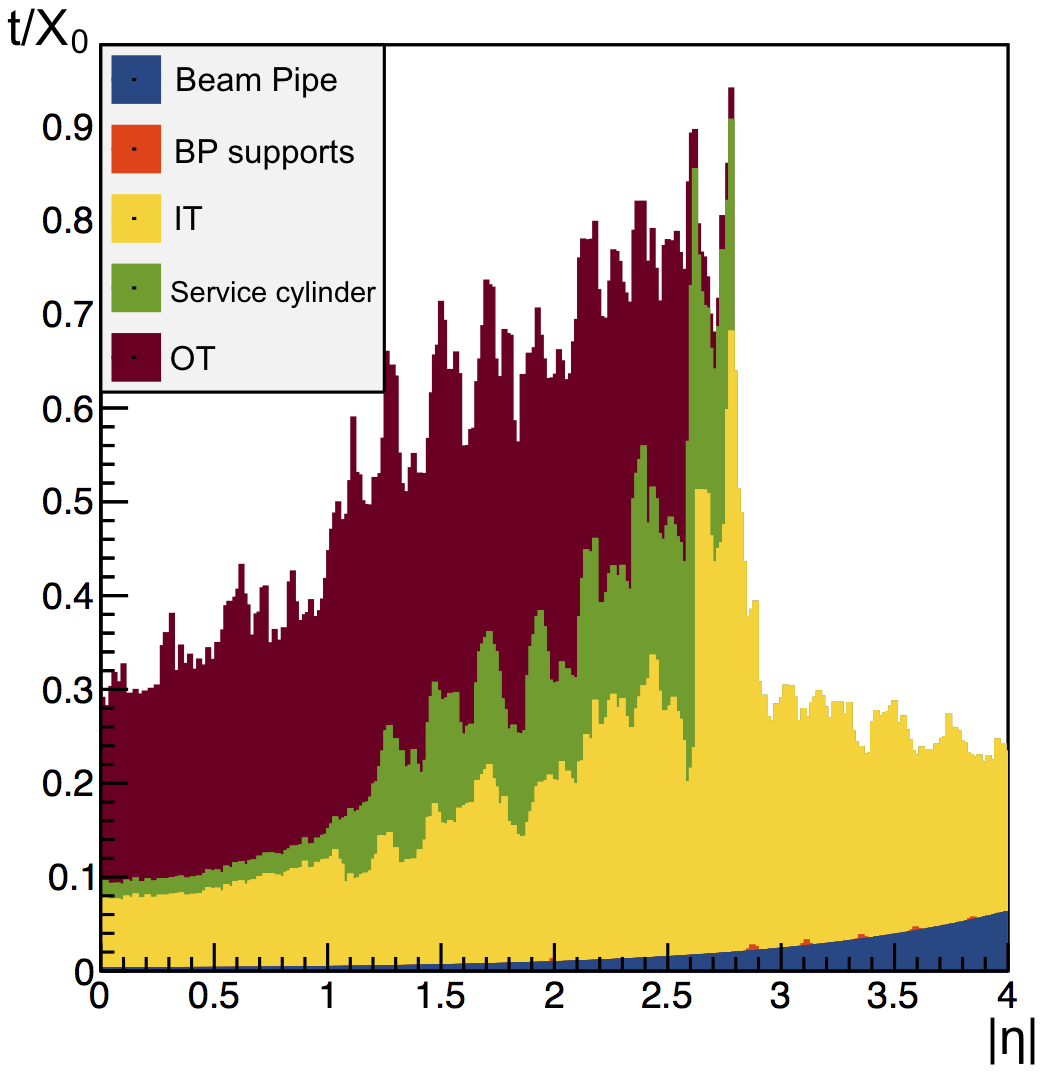
\includegraphics[width=0.4\textwidth]{Immagini/MBfase2.png}
\caption{Spessore totale $t$ del tracciatore di CMS di fase-2 in unit\`a di lunghezza di radiazione $X_0$ in funzione di $\eta$.}
\label{fig:MBfase2}
\end{figure}

